\section{Hastighetsregulator}\label{sec:hastighetsreg}


\subsection{Teori}

Regulatorer brukes for å styre tilstander i en prosess. En regulator får inn et avvik mellom referansen og den målte tilstanden. Regulatorer bruker avviket til å beregne et pådrag til prosessen. P-regulator er en type regulator som lager et pådrag, $u$,  som er proporsjonalt med avviket, $e = \omega_d - \omega_m$. $K_p$ er proporsjonalforstkerningen i regulatoren. Uttrykket for denne regulatoren er slik

\begin{equation}
    \label{eq:P_regulator}
    u(t) = K_p e(t).
\end{equation}

En slik regulator er effektiv så lenge det ikke er en kraft som forhindrer systemet å oppnå en spesifikk tilstand. Med en slik kraft vil ikke regulatoren regulere tilstanden helt til referanseverdien og det oppstår et stasjonæravvik. Friksjon og luftmotstand er krefter som vil motvirke at et system oppnår en hastighet større enn $0$. Et integratorledd vil motvirke slike krefter, ved å gi et pådrag tilsvarende disse kreftene. Da vil tilstanden nå referansen og det stasjonære avviket forsvinner. Uttrykk \eqref{eq:PI_regulator} beskriver en PI-regulator,

\begin{equation}
    \label{eq:PI_regulator}
    u(t) = K_p e(t) + \frac{K_p}{T_i} \int_{0}^{t} e(\tau) d\tau,
\end{equation}

der $u$ er pådraget, $K_p$ er proporsjonalitetskontanten, $e$ er avviket mellom referansen og tilstanden og $T_i$ er integratorkonstanten som representerer tidskonstanten til regulatoren.







\subsection{Metode}

\begin{figure}[b]
    \centering
    \begin{circuitikz} [scale=0.5, transform shape]
    \ctikzset{resistor = european}

    % --- OP1 ---
    \node[op amp](OP1) {$OP1$};
    
    \draw (OP1.-)
    to[R, l_=$R_1$] ++(-2, 0)
    to[short, o-, l=$\omega_m$] ++(0, 0);

    \draw (OP1.+)
    to[R=$R_1$] ++(-2, 0)
    to[short, o-, l=$\omega_d$] ++(0, 0);

    \draw (OP1.+)
    to[R=$R_2$, *-] ++(0, -2)
    node[ground] {};

    \draw (OP1.-)
    to[short, *-] ++(0, 1)
    coordinate(t1)
    to[R=$R_2$] (t1 -| OP1.out)
    -- (OP1.out);

    % --- OP2 ---

    \draw (OP1.out)
    to[short, *-, l=$e$] ++(0.5, 0)
    to[R=$R_3$] ++(2, 0)
    node[op amp, anchor=-](OP2) {$OP2$};

    \draw (OP2.-)
    to[short, *-] ++(0, 1)
    coordinate(t2)
    to[R=$R_4$] (t2 -| OP2.out)
    -- (OP2.out);

    \draw (OP2.+)
    node[ground] {};

    \draw (OP2.out)
    to[short, *-] ++(0, 0)
    to[R=$R7$] ++(0, -2)
    coordinate(t7);

    % --- OP3 ---

    \draw (OP1.out)
    -- ++(0, -2)
    to[potentiometer, n=R5, l=$R_5$] ++(0, -2)
    coordinate(t3);

    \draw (R5.wiper)
    -- (R5.wiper |- t3)
    -- (t3);

    \draw (t3)
    to[short, *-] ++(0, -1)
    to[R=$R_6$] ++(2, 0)
    node[op amp, anchor=-](OP3) {$OP3$};

    \draw (OP3.+)
    node[ground] {};
    
    \draw (OP3.-)
    to[short, *-] ++(0, 1)
    coordinate(t4)
    to[C=$C_1$] (t4 -| OP3.out)
    coordinate(t5)
    -- (OP3.out);

    \draw (t4)
    to[short, *-] ++(0, 1.3)
    coordinate(t6)
    to[open jumper, l=$JP1$] (t6 -| t5)
    to[short, -*] (t5);

    \draw (OP3.out)
    to[short, *-] (OP3.out -| OP2.out)
    to[R, l_=$R7$] ++(0, 2)
    coordinate (t8)
    to[short, *-*] (t7);

    % --- OP4 ---

    \draw (t8)
    -- ++(1.5, 0)
    node[op amp, anchor=-](OP4) {$OP4$};

    \draw (OP4.+)
    node[ground] {};

    \draw (t7)
    to[R=$R8$] ++(2, 0)
    coordinate(t9)
    to[potentiometer, n=R9, l=$R9$] (t9 -| OP4.out)
    coordinate(t10)
    -- (OP4.out);

    \draw (R9.wiper)
    -- (R9.wiper -| t10)
    to[short, -*] (t10);

    \draw (OP4.out)
    to[short, *-o, l=$V_m$] ++(1, 0);
    
\end{circuitikz}
    \caption{PI-regulator krets for hastighetsregulatoren. Figuren er hentet fra \cite{AnalogMotorlabbOppgaver}.}
    \label{fig:krets_hastighets_regulator}
\end{figure}

Hastighetsregulatoren ble implementert som en analog PI-regulator som vist i \autoref{fig:krets_hastighets_regulator}, med verdier for komponentene som i \autoref{tab:Komponenter_i_hastighetsregulatoren}. $OP1$ er en differensialforsterker som finner avviket $e$, transferfunksjonen er gitt ved \eqref{eq:differensialforsterker}.
$OP2$ er en inverterende forsterker som inverterer avviket, uten forsterkning eller demping.
$OP3$ er en integrerende forsterker som integrerer $e$ og forsterker den med $\frac{1}{T_i}$.
$JP1$ brukes for å nullstille integratoren og skru av I-leddet i regulatoren.
Da vil spenningen ut fra $OP3$ være \SI{0}{\volt} \cite{AnalogMotorlabbOppgaver}.
Da vil regulatoren oppføre seg som en P-regulator.
Transferfunksjonen til $OP3$ blir $-\frac{1}{(R_5 + R_6) C_1} \int^t_0 e(\tau) d\tau$ \cite{Johnson}.
$OP4$ summerer spenningen fra $OP2$ og $OP3$ og forsterker resultatet med $K_p$.
Transferfunksjonen for $OP4$ er $-\frac{R_8 + R_9}{R_7}(v_2 + v_3)$ \cite{Johnson}, der $v_2$ er spenningen ut av $OP2$ og $v_3$ er spenningen ut av $OP3$. 
Da blir transerfunksjonen for hele kretsen slik

\begin{equation}
    \label{eq:hastighet_regulator_transferfuksjon}
    V_m =
    \frac{R_2}{R_1} \frac{R_8 + R_9}{R_7} \left(e + \frac{1}{(R_5 + R_6) C_1} \int^t_0 e(\tau) d\tau \right),
\end{equation}

der $e = \omega_m - \omega_d$
Dette gir oss følgende uttrykk for $K_p$ og $T_i$,

\begin{equation}
    \label{eq:K_p_og_T_i}
    K_p = \frac{R_2}{R_1} \frac{R_8 + R_9}{R_7}, 
    T_i = (R_5 + R_6) C_1.
\end{equation}

\begin{table}[h]
    \centering
    \caption{Motstander og kondensatorer i hastighetsregulatoren. Verdiene er hentet fra \cite{AnalogMotorlabbOppgaver}.}
    \begin{tabular}{lll}
        \toprule
        Størrelse & Verdi & Type \\
		\midrule
        $R_1$, $R_2$ & \SI{100}{\kilo\ohm} & Resistor\\
        $R_3$, $R_4$, $R_7$, $R_8$ & \SI{10}{\kilo\ohm} & Resistor \\
        $R_5$, $R_9$ & \SI{1}{\mega\ohm} & Potmeter \\
        $R_6$ & \SI{1}{\kilo\ohm} & Resistor \\
        $C_1$ & \SI{1}{\micro\farad} & Kondensator \\
        \bottomrule
    \end{tabular}
    \label{tab:Komponenter_i_hastighetsregulatoren}
\end{table}






\subsection{Resultater}

\label{obs:hastighet_regulator_breming_med_finger}
Da motoren ble bremset med en finger økte både pådraget og stasjonæravviket når integratorleddet var skrudd av. Ved bruk av integratorleddet økte pådraget helt til tilstanden nådde referanseverdien.

\begin{figure}[h]
    \centering
    % This file was created with tikzplotlib v0.10.1.
% Dette er eksempel data
\begin{tikzpicture}

\definecolor{darkgray176}{RGB}{176,176,176}
\definecolor{darkorange25512714}{RGB}{255,127,14}
\definecolor{steelblue31119180}{RGB}{31,119,180}

\begin{axis}[
tick align=outside,
tick pos=left,
title={Hastighet P-regulator},
legend pos=south east,
height=\figH,
width=\figW,
x grid style={darkgray176},
xlabel={Tid [ms]},
xmin=-11.54538, xmax=242.45298,
xtick style={color=black},
xtick={-50,0,50,100,150,200,250},
xticklabels={
  \(\displaystyle {\ensuremath{-}50}\),
  \(\displaystyle {0}\),
  \(\displaystyle {50}\),
  \(\displaystyle {100}\),
  \(\displaystyle {150}\),
  \(\displaystyle {200}\),
  \(\displaystyle {250}\)
},
y grid style={darkgray176},
ylabel={Spenning [V]},
ymin=-10.231936, ymax=10.231936,
ytick style={color=black},
ytick={-12.5,-10,-7.5,-5,-2.5,0,2.5,5,7.5,10,12.5},
yticklabels={
  \(\displaystyle {\ensuremath{-}12.5}\),
  \(\displaystyle {\ensuremath{-}10.0}\),
  \(\displaystyle {\ensuremath{-}7.5}\),
  \(\displaystyle {\ensuremath{-}5.0}\),
  \(\displaystyle {\ensuremath{-}2.5}\),
  \(\displaystyle {0.0}\),
  \(\displaystyle {2.5}\),
  \(\displaystyle {5.0}\),
  \(\displaystyle {7.5}\),
  \(\displaystyle {10.0}\),
  \(\displaystyle {12.5}\)
}
]
\legend{$\omega_m$, $\omega_d$}
\addplot [semithick, steelblue31119180]
table {%
0 -8.42285
0.2772000000002 -8.37402
0.554400000000399 -8.22754
0.83159999999971 -8.47168
1.10879999999991 -8.42285
1.38600000000011 -8.42285
1.66320000000031 -8.37402
1.94039999999962 -8.12988
2.21759999999982 -8.22754
2.49480000000002 -8.47168
2.77200000000022 -8.37402
3.04919999999953 -8.47168
3.32639999999973 -8.22754
3.60359999999993 -8.42285
3.88080000000013 -8.3252
4.15800000000033 -8.61816
4.43519999999964 -8.3252
4.71239999999984 -8.27637
4.98960000000004 -8.37402
5.26680000000024 -8.47168
5.54399999999955 -8.52051
5.82119999999975 -8.42285
6.09839999999995 -8.3252
6.37560000000015 -8.12988
6.65280000000035 -8.37402
6.92999999999966 -8.42285
7.20719999999986 -8.37402
7.48440000000006 -8.3252
7.76160000000026 -8.17871
8.03879999999957 -8.37402
8.31599999999977 -8.37402
8.59319999999997 -8.42285
8.87040000000017 -8.42285
9.14760000000037 -8.42285
9.42479999999968 -8.52051
9.70199999999988 -8.47168
9.97920000000008 -8.22754
10.2564000000003 -8.3252
10.5335999999996 -8.37402
10.8107999999998 -8.42285
11.088 -8.47168
11.3652000000002 -8.61816
11.6424000000004 -8.22754
11.9195999999997 -8.17871
12.1967999999999 -8.27637
12.4740000000001 -8.42285
12.7512000000003 -8.3252
13.0283999999996 -8.42285
13.3055999999998 -8.27637
13.5828 -8.42285
13.8600000000002 -8.37402
14.1371999999995 -8.61816
14.4143999999997 -8.3252
14.6915999999999 -8.22754
14.9688000000001 -8.42285
15.2460000000003 -8.47168
15.5231999999996 -8.42285
15.8003999999998 -8.47168
16.0776 -8.22754
16.3548000000002 -8.42285
16.6319999999995 -8.56934
16.9091999999997 -8.3252
17.1863999999999 -8.37402
17.4636000000001 -8.3252
17.7408000000003 -8.27637
18.0179999999996 -8.47168
18.2951999999998 -8.3252
18.5724 -8.47168
18.8496000000002 -8.17871
19.1267999999996 -8.42285
19.4039999999998 -8.37402
19.6812 -8.42285
19.9584000000002 -8.22754
20.2356000000004 -8.12988
20.5127999999997 -8.42285
20.7899999999999 -8.61816
21.0672000000001 -8.52051
21.3444000000003 -8.47168
21.6215999999996 -8.08105
21.8987999999998 -8.12988
22.176 -8.3252
22.4532000000002 -8.22754
22.7304000000004 -8.3252
23.0075999999997 -8.37402
23.2847999999999 -8.17871
23.5620000000001 -8.3252
23.8392000000003 -8.22754
24.1163999999996 -8.42285
24.3935999999998 -8.27637
24.6708 -8.17871
24.9480000000002 -8.3252
25.2252000000004 -8.61816
25.5023999999997 -8.27637
25.7795999999999 -8.42285
26.0568000000001 -8.27637
26.3340000000003 -8.47168
26.6111999999996 -8.52051
26.8883999999998 -8.37402
27.1656 -8.22754
27.4428000000002 -8.42285
27.7199999999995 -8.42285
27.9971999999997 -8.42285
28.2743999999999 -8.37402
28.5516000000001 -8.42285
28.8288000000003 -8.42285
29.1059999999996 -8.27637
29.3831999999998 -8.52051
29.6604 -8.27637
29.9376000000002 -8.3252
30.2147999999995 -8.42285
30.4919999999997 -8.42285
30.7691999999999 -8.42285
31.0464000000001 -8.3252
31.3236000000003 -8.56934
31.6007999999997 -8.03223
31.8779999999999 -8.42285
32.1552000000001 -8.22754
32.4324000000002 -8.22754
32.7095999999996 -8.08105
32.9867999999998 -8.42285
33.264 -8.42285
33.5412000000002 -8.42285
33.8184000000004 -8.47168
34.0955999999997 -8.52051
34.3727999999999 -8.3252
34.6500000000001 -8.47168
34.9272000000003 -8.3252
35.2043999999996 -8.56934
35.4815999999998 -8.37402
35.7588 -8.37402
36.0360000000002 -8.3252
36.3132000000004 -8.61816
36.5903999999997 -8.3252
36.8675999999999 -8.27637
37.1448000000001 -8.22754
37.4220000000003 -8.42285
37.6991999999996 -8.56934
37.9763999999998 -8.56934
38.2536 -8.42285
38.5308000000002 -8.12988
38.8080000000004 -8.37402
39.0851999999997 -8.42285
39.3623999999999 -8.27637
39.6396000000001 -8.3252
39.9168000000003 -8.22754
40.1939999999996 -8.47168
40.4711999999998 -8.42285
40.7484 -8.42285
41.0256000000002 -8.22754
41.3027999999995 -7.93457
41.5799999999997 -8.37402
41.8571999999999 -8.42285
42.1344000000001 -8.52051
42.4116000000003 -8.22754
42.6887999999996 -8.22754
42.9659999999998 -8.42285
43.2432 -8.52051
43.5204000000002 -8.37402
43.7975999999995 -8.37402
44.0747999999997 -8.27637
44.3519999999999 -8.3252
44.6292000000001 -8.61816
44.9064000000003 -8.52051
45.1835999999997 -8.66699
45.4607999999999 -8.3252
45.7380000000001 -8.22754
46.0152000000003 -8.37402
46.2923999999996 -8.3252
46.5695999999998 -8.42285
46.8468 -8.56934
47.1240000000002 -8.52051
47.4012000000004 -8.42285
47.6783999999997 -8.3252
47.9555999999999 -8.42285
48.2328000000001 -8.08105
48.5100000000003 -8.3252
48.7871999999996 -8.37402
49.0643999999998 -8.42285
49.3416 -8.37402
49.6188000000002 -8.3252
49.8960000000004 -8.42285
50.1731999999997 -8.81348
50.4503999999999 -8.52051
50.7276000000001 -8.22754
51.0048000000003 -8.27637
51.2819999999996 -8.22754
51.5591999999998 -8.22754
51.8364 -8.42285
52.1136000000002 -8.3252
52.3907999999995 -8.17871
52.6679999999997 -8.22754
52.9451999999999 -8.42285
53.2224000000001 -8.47168
53.4996000000003 -8.27637
53.7767999999996 -8.27637
54.0539999999998 -8.27637
54.3312 -8.37402
54.6084000000002 -8.61816
54.8855999999995 -8.27637
55.1627999999997 -8.37402
55.4399999999999 -8.08105
55.7172000000001 -8.37402
55.9944000000003 -8.3252
56.2715999999996 -8.47168
56.5487999999998 -8.3252
56.826 -8.22754
57.1032000000002 -8.37402
57.3803999999996 -8.61816
57.6575999999998 -8.37402
57.9348 -8.47168
58.2120000000002 -8.27637
58.4892000000004 -8.52051
58.7663999999997 -8.37402
59.0435999999999 -8.42285
59.3208000000001 -8.27637
59.5980000000003 -8.12988
59.8751999999996 -8.42285
60.1523999999998 -8.3252
60.4296 -8.42285
60.7068000000002 -8.42285
60.9840000000004 -8.17871
61.2611999999997 -8.27637
61.5383999999999 -8.42285
61.8156000000001 -8.42285
62.0928000000003 -8.22754
62.3699999999996 -8.22754
62.6471999999998 -8.3252
62.9244 -8.42285
63.2016000000002 -8.27637
63.4788000000004 -8.42285
63.7559999999997 -8.3252
64.0331999999999 -8.37402
64.3104000000001 -8.42285
64.5876000000003 -8.42285
64.8647999999996 -8.27637
65.1419999999998 -8.42285
65.4192 -8.42285
65.6964000000002 -8.47168
65.9735999999995 -8.3252
66.2507999999997 -8.42285
66.5279999999999 -8.22754
66.8052000000001 -8.42285
67.0824000000003 -8.42285
67.3595999999996 -8.56934
67.6367999999998 -8.37402
67.914 -8.3252
68.1912000000002 -8.42285
68.4683999999995 -8.42285
68.7455999999997 -8.37402
69.0227999999999 -8.47168
69.3000000000001 -8.27637
69.5772000000003 -8.47168
69.8543999999997 -8.42285
70.1315999999998 -8.37402
70.4088 -8.47168
70.6860000000002 -8.22754
70.9631999999996 -8.22754
71.2403999999998 -8.52051
71.5176 -8.3252
71.7948000000002 -8.17871
72.0720000000004 -8.12988
72.3491999999997 -8.42285
72.6263999999999 -8.27637
72.9036000000001 -8.52051
73.1808000000003 -8.37402
73.4579999999996 -8.42285
73.7351999999998 -8.37402
74.0124 -8.47168
74.2896000000002 -8.22754
74.5668000000004 -8.47168
74.8439999999997 -8.12988
75.1211999999999 -8.42285
75.3984000000001 -8.42285
75.6756000000003 -8.52051
75.9527999999996 -8.37402
76.2299999999998 -8.37402
76.5072 -8.22754
76.7844000000002 -8.56934
77.0616000000004 -8.47168
77.3387999999997 -8.47168
77.6159999999999 -8.08105
77.8932000000001 -8.22754
78.1704000000003 -8.52051
78.4475999999996 -8.61816
78.7247999999998 -8.37402
79.002 -8.22754
79.2792000000002 -8.08105
79.5563999999995 -8.03223
79.8335999999997 -7.93457
80.1107999999999 -7.88574
80.3880000000001 -7.59277
80.6652000000003 -7.34863
80.9423999999996 -7.34863
81.2195999999998 -7.20215
81.4968 -7.15332
81.7740000000002 -7.25098
82.0511999999995 -6.90918
82.3283999999997 -6.81152
82.6056 -6.81152
82.8828000000001 -6.66504
83.1600000000003 -6.7627
83.4371999999996 -6.46973
83.7143999999999 -6.4209
83.9916000000001 -6.0791
84.2688000000003 -6.22559
84.5459999999996 -6.12793
84.8231999999998 -6.03027
85.1004 -5.88379
85.3776000000002 -5.78613
85.6548000000004 -5.83496
85.9319999999997 -5.49316
86.2091999999999 -5.34668
86.4864000000001 -5.29785
86.7636000000003 -5.2002
87.0407999999996 -5.24902
87.3179999999998 -5.00488
87.5952 -5.00488
87.8724000000002 -4.8584
88.1496000000004 -4.8584
88.4267999999997 -4.76074
88.7039999999999 -4.71191
88.9812000000001 -4.41895
89.2584000000003 -4.37012
89.5355999999996 -4.27246
89.8127999999998 -4.22363
90.09 -4.12598
90.3672000000002 -4.22363
90.6443999999995 -3.88184
90.9215999999997 -3.78418
91.1987999999999 -3.6377
91.4760000000001 -3.73535
91.7532000000003 -3.49121
92.0303999999996 -3.34473
92.3075999999998 -3.34473
92.5848 -3.19824
92.8620000000002 -3.00293
93.1391999999995 -2.90527
93.4163999999997 -2.75879
93.6935999999999 -2.80762
93.9708000000001 -2.56348
94.2480000000003 -2.51465
94.5251999999996 -2.36816
94.8023999999998 -2.17285
95.0796 -2.22168
95.3568000000002 -2.17285
95.6339999999996 -1.97754
95.9111999999998 -1.92871
96.1883999999999 -1.78223
96.4656000000002 -1.78223
96.7428000000004 -1.53809
97.0199999999997 -1.48926
97.2971999999999 -1.48926
97.5744000000001 -1.34277
97.8516000000003 -1.29395
98.1287999999996 -1.24512
98.4059999999998 -1.00098
98.6832 -0.952148
98.9604000000002 -0.952148
99.2376000000004 -0.708008
99.5147999999997 -0.65918
99.7919999999999 -0.512695
100.0692 -0.561523
100.3464 -0.268555
100.6236 -0.268555
100.9008 -0.12207
101.178 -0.0732422
101.4552 0.12207
101.7324 0.170898
102.0096 0.415039
102.2868 0.366211
102.564 0.366211
102.8412 0.561523
103.1184 0.708008
103.3956 0.805664
103.6728 0.805664
103.95 0.854492
104.2272 1.19629
104.5044 1.29395
104.7816 1.29395
105.0588 1.44043
105.336 1.44043
105.6132 1.44043
105.8904 1.58691
106.1676 1.7334
106.4448 1.83105
106.722 1.83105
106.9992 1.97754
107.2764 1.97754
107.5536 1.97754
107.8308 2.31934
108.108 2.41699
108.3852 2.36816
108.6624 2.51465
108.9396 2.6123
109.2168 2.66113
109.494 2.85645
109.7712 2.85645
110.0484 2.85645
110.3256 3.10059
110.6028 2.9541
110.88 3.14941
111.1572 3.19824
111.4344 3.39355
111.7116 3.44238
111.9888 3.54004
112.266 3.6377
112.5432 3.6377
112.8204 3.93066
113.0976 3.83301
113.3748 4.02832
113.652 4.12598
113.9292 4.07715
114.2064 4.1748
114.4836 4.22363
114.7608 4.27246
115.038 4.22363
115.3152 4.46777
115.5924 4.5166
115.8696 4.56543
116.1468 4.76074
116.424 4.90723
116.7012 4.71191
116.9784 4.66309
117.2556 4.80957
117.5328 4.95605
117.81 5.05371
118.0872 5.10254
118.3644 5.2002
118.6416 5.34668
118.9188 5.24902
119.196 5.34668
119.4732 5.34668
119.7504 5.44434
120.0276 5.49316
120.3048 5.63965
120.582 5.59082
120.8592 5.88379
121.1364 5.7373
121.4136 5.7373
121.6908 5.63965
121.968 5.7373
122.2452 5.88379
122.5224 5.93262
122.7996 6.03027
123.0768 6.12793
123.354 5.98145
123.6312 6.12793
123.9084 6.17676
124.1856 6.27441
124.4628 6.37207
124.74 6.46973
125.0172 6.37207
125.2944 6.37207
125.5716 6.32324
125.8488 6.46973
126.126 6.51855
126.4032 6.66504
126.6804 6.7627
126.9576 6.66504
127.2348 6.51855
127.512 6.81152
127.7892 6.7627
128.0664 7.00684
128.3436 6.86035
128.6208 7.10449
128.898 6.61621
129.1752 6.7627
129.4524 6.86035
129.7296 7.20215
130.0068 7.05566
130.284 6.95801
130.5612 6.95801
130.8384 7.10449
131.1156 7.10449
131.3928 7.15332
131.67 7.34863
131.9472 7.34863
132.2244 7.15332
132.5016 7.44629
132.7788 7.34863
133.056 7.25098
133.3332 7.44629
133.6104 7.34863
133.8876 7.39746
134.1648 7.34863
134.442 7.54395
134.7192 7.54395
134.9964 7.54395
135.2736 7.54395
135.5508 7.54395
135.828 7.78809
136.1052 7.73926
136.3824 7.88574
136.6596 7.78809
136.9368 7.78809
137.214 7.73926
137.4912 7.78809
137.7684 7.83691
138.0456 7.9834
138.3228 7.73926
138.6 7.83691
138.8772 8.03223
139.1544 8.3252
139.4316 8.08105
139.7088 7.9834
139.986 8.12988
140.2632 8.12988
140.5404 8.03223
140.8176 8.22754
141.0948 8.12988
141.372 7.9834
141.6492 8.12988
141.9264 8.22754
142.2036 8.3252
142.4808 8.22754
142.758 8.08105
143.0352 8.12988
143.3124 8.12988
143.5896 8.22754
143.8668 8.27637
144.144 8.22754
144.4212 8.08105
144.6984 8.42285
144.9756 8.22754
145.2528 8.37402
145.53 8.3252
145.8072 8.17871
146.0844 8.52051
146.3616 8.56934
146.6388 8.42285
146.916 8.42285
147.1932 8.3252
147.4704 8.3252
147.7476 8.42285
148.0248 8.37402
148.302 8.22754
148.5792 8.3252
148.8564 8.37402
149.1336 8.52051
149.4108 8.3252
149.688 8.22754
149.9652 8.22754
150.2424 8.42285
150.5196 8.37402
150.7968 8.42285
151.074 8.3252
151.3512 8.17871
151.6284 8.22754
151.9056 8.52051
152.1828 8.3252
152.46 8.3252
152.7372 8.27637
153.0144 8.42285
153.2916 8.56934
153.5688 8.37402
153.846 8.3252
154.1232 8.3252
154.4004 8.3252
154.6776 8.56934
154.9548 8.52051
155.232 8.37402
155.5092 8.3252
155.7864 8.27637
156.0636 8.52051
156.3408 8.3252
156.618 8.47168
156.8952 8.22754
157.1724 8.22754
157.4496 8.37402
157.7268 8.42285
158.004 8.37402
158.2812 8.27637
158.5584 8.52051
158.8356 8.61816
159.1128 8.42285
159.39 8.42285
159.6672 8.47168
159.9444 8.08105
160.2216 8.42285
160.4988 8.56934
160.776 8.47168
161.0532 8.22754
161.3304 8.3252
161.6076 8.37402
161.8848 8.52051
162.162 8.37402
162.4392 8.3252
162.7164 8.22754
162.9936 8.22754
163.2708 8.42285
163.548 8.47168
163.8252 8.17871
164.1024 8.12988
164.3796 8.17871
164.6568 8.42285
164.934 8.37402
165.2112 8.27637
165.4884 8.08105
165.7656 8.52051
166.0428 8.52051
166.32 8.61816
166.5972 8.37402
166.8744 8.22754
167.1516 8.37402
167.4288 8.27637
167.706 8.42285
167.9832 8.37402
168.2604 8.12988
168.5376 8.27637
168.8148 8.22754
169.092 8.42285
169.3692 8.37402
169.6464 8.22754
169.9236 8.37402
170.2008 8.47168
170.478 8.3252
170.7552 8.27637
171.0324 8.37402
171.3096 8.42285
171.5868 8.47168
171.864 8.52051
172.1412 8.37402
172.4184 8.17871
172.6956 8.37402
172.9728 8.47168
173.25 8.42285
173.5272 8.47168
173.8044 8.22754
174.0816 8.17871
174.3588 8.42285
174.636 8.37402
174.9132 8.27637
175.1904 8.3252
175.4676 8.27637
175.7448 8.61816
176.022 8.42285
176.2992 8.56934
176.5764 8.37402
176.8536 8.12988
177.1308 8.37402
177.408 8.3252
177.6852 8.37402
177.9624 8.42285
178.2396 8.52051
178.5168 8.52051
178.794 8.3252
179.0712 8.42285
179.3484 8.12988
179.6256 8.17871
179.9028 8.3252
180.18 8.47168
180.4572 8.37402
180.7344 8.27637
181.0116 8.3252
181.2888 8.42285
181.566 8.42285
181.8432 8.47168
182.1204 8.37402
182.3976 8.17871
182.6748 8.42285
182.952 8.47168
183.2292 8.42285
183.5064 8.27637
183.7836 8.03223
184.0608 8.27637
184.338 8.27637
184.6152 8.42285
184.8924 8.37402
185.1696 8.22754
185.4468 8.42285
185.724 8.56934
186.0012 8.61816
186.2784 8.47168
186.5556 8.22754
186.8328 8.47168
187.11 8.17871
187.3872 8.42285
187.6644 8.37402
187.9416 8.17871
188.2188 8.3252
188.496 8.3252
188.7732 8.3252
189.0504 8.47168
189.3276 8.37402
189.6048 8.22754
189.882 8.52051
190.1592 8.37402
190.4364 8.37402
190.7136 8.22754
190.9908 8.3252
191.268 8.3252
191.5452 8.37402
191.8224 8.3252
192.0996 8.12988
192.3768 8.37402
192.654 8.27637
192.9312 8.47168
193.2084 8.52051
193.4856 8.22754
193.7628 8.22754
194.04 8.27637
194.3172 8.37402
194.5944 8.37402
194.8716 8.17871
195.1488 8.42285
195.426 8.52051
195.7032 8.56934
195.9804 8.3252
196.2576 8.37402
196.5348 8.27637
196.812 8.3252
197.0892 8.42285
197.3664 8.42285
197.6436 8.37402
197.9208 8.27637
198.198 8.42285
198.4752 8.47168
198.7524 8.52051
199.0296 8.47168
199.3068 8.12988
199.584 8.42285
199.8612 8.3252
200.1384 8.42285
200.4156 8.27637
200.6928 8.22754
200.97 8.37402
201.2472 8.56934
201.5244 8.37402
201.8016 8.27637
202.0788 8.22754
202.356 8.37402
202.6332 8.42285
202.9104 8.42285
203.1876 8.37402
203.4648 8.22754
203.742 8.37402
204.0192 8.42285
204.2964 8.42285
204.5736 8.37402
204.8508 8.22754
205.128 8.42285
205.4052 8.42285
205.6824 8.56934
205.9596 8.52051
206.2368 8.27637
206.514 8.37402
206.7912 8.37402
207.0684 8.47168
207.3456 8.27637
207.6228 8.17871
207.9 8.47168
208.1772 8.37402
208.4544 8.37402
208.7316 8.42285
209.0088 8.17871
209.286 8.17871
209.5632 8.37402
209.8404 8.52051
210.1176 8.42285
210.3948 8.52051
210.672 8.12988
210.9492 8.37402
211.2264 8.27637
211.5036 8.42285
211.7808 8.12988
212.058 8.37402
212.3352 8.42285
212.6124 8.3252
212.8896 8.52051
213.1668 8.22754
213.444 8.17871
213.7212 8.27637
213.9984 8.42285
214.2756 8.37402
214.5528 8.37402
214.83 8.3252
215.1072 8.42285
215.3844 8.56934
215.6616 8.42285
215.9388 8.27637
216.216 8.22754
216.4932 8.37402
216.7704 8.56934
217.0476 8.37402
217.3248 8.22754
217.602 8.27637
217.8792 8.47168
218.1564 8.52051
218.4336 8.42285
218.7108 8.3252
218.988 8.3252
219.2652 8.17871
219.5424 8.37402
219.8196 8.3252
220.0968 8.42285
220.374 8.27637
220.6512 8.42285
220.9284 8.47168
221.2056 8.42285
221.4828 8.3252
221.76 8.17871
222.0372 8.12988
222.3144 8.42285
222.5916 8.66699
222.8688 8.37402
223.146 8.08105
223.4232 8.27637
223.7004 8.17871
223.9776 8.27637
224.2548 8.27637
224.532 8.22754
224.8092 8.22754
225.0864 8.56934
225.3636 8.61816
225.6408 8.66699
225.918 8.17871
226.1952 8.27637
226.4724 8.42285
226.7496 8.47168
227.0268 8.42285
227.304 8.12988
227.5812 8.22754
227.8584 8.42285
228.1356 8.3252
228.4128 8.27637
228.69 8.22754
228.9672 8.3252
229.2444 8.42285
229.5216 8.56934
229.7988 8.37402
230.076 8.27637
230.3532 8.12988
230.6304 8.42285
230.9076 8.42285
};
\addplot [semithick, darkorange25512714]
table {%
0 -8.95996
0.2772000000002 -9.05762
0.554400000000399 -9.10645
0.83159999999971 -9.30176
1.10879999999991 -9.2041
1.38600000000011 -9.15527
1.66320000000031 -9.05762
1.94039999999962 -8.95996
2.21759999999982 -9.2041
2.49480000000002 -9.2041
2.77200000000022 -8.95996
3.04919999999953 -9.05762
3.32639999999973 -8.95996
3.60359999999993 -9.15527
3.88080000000013 -9.2041
4.15800000000033 -9.30176
4.43519999999964 -8.95996
4.71239999999984 -9.25293
4.98960000000004 -9.10645
5.26680000000024 -9.10645
5.54399999999955 -9.00879
5.82119999999975 -9.10645
6.09839999999995 -9.10645
6.37560000000015 -9.15527
6.65280000000035 -9.10645
6.92999999999966 -9.05762
7.20719999999986 -9.10645
7.48440000000006 -9.15527
7.76160000000026 -9.10645
8.03879999999957 -9.2041
8.31599999999977 -8.95996
8.59319999999997 -9.15527
8.87040000000017 -8.95996
9.14760000000037 -9.05762
9.42479999999968 -9.10645
9.70199999999988 -9.15527
9.97920000000008 -9.25293
10.2564000000003 -9.15527
10.5335999999996 -9.25293
10.8107999999998 -9.2041
11.088 -9.10645
11.3652000000002 -9.10645
11.6424000000004 -9.00879
11.9195999999997 -9.10645
12.1967999999999 -9.10645
12.4740000000001 -9.2041
12.7512000000003 -9.15527
13.0283999999996 -9.10645
13.3055999999998 -8.95996
13.5828 -9.2041
13.8600000000002 -9.05762
14.1371999999995 -9.00879
14.4143999999997 -9.00879
14.6915999999999 -9.05762
14.9688000000001 -9.10645
15.2460000000003 -8.95996
15.5231999999996 -9.05762
15.8003999999998 -9.2041
16.0776 -9.10645
16.3548000000002 -9.15527
16.6319999999995 -9.05762
16.9091999999997 -9.2041
17.1863999999999 -9.10645
17.4636000000001 -9.10645
17.7408000000003 -9.10645
18.0179999999996 -9.25293
18.2951999999998 -9.10645
18.5724 -9.25293
18.8496000000002 -9.2041
19.1267999999996 -9.05762
19.4039999999998 -9.25293
19.6812 -9.00879
19.9584000000002 -8.95996
20.2356000000004 -9.25293
20.5127999999997 -9.05762
20.7899999999999 -9.25293
21.0672000000001 -9.30176
21.3444000000003 -9.10645
21.6215999999996 -9.10645
21.8987999999998 -9.15527
22.176 -9.2041
22.4532000000002 -9.10645
22.7304000000004 -9.15527
23.0075999999997 -9.00879
23.2847999999999 -9.10645
23.5620000000001 -9.10645
23.8392000000003 -9.10645
24.1163999999996 -9.15527
24.3935999999998 -9.2041
24.6708 -9.15527
24.9480000000002 -9.15527
25.2252000000004 -9.15527
25.5023999999997 -9.10645
25.7795999999999 -8.95996
26.0568000000001 -9.25293
26.3340000000003 -9.10645
26.6111999999996 -9.10645
26.8883999999998 -9.25293
27.1656 -9.2041
27.4428000000002 -9.15527
27.7199999999995 -8.95996
27.9971999999997 -9.10645
28.2743999999999 -9.15527
28.5516000000001 -9.10645
28.8288000000003 -9.2041
29.1059999999996 -9.00879
29.3831999999998 -9.10645
29.6604 -9.05762
29.9376000000002 -9.30176
30.2147999999995 -9.25293
30.4919999999997 -9.00879
30.7691999999999 -9.2041
31.0464000000001 -9.10645
31.3236000000003 -9.10645
31.6007999999997 -9.10645
31.8779999999999 -8.95996
32.1552000000001 -9.10645
32.4324000000002 -9.2041
32.7095999999996 -9.05762
32.9867999999998 -9.25293
33.264 -9.10645
33.5412000000002 -9.30176
33.8184000000004 -8.95996
34.0955999999997 -9.10645
34.3727999999999 -9.00879
34.6500000000001 -9.25293
34.9272000000003 -9.10645
35.2043999999996 -9.15527
35.4815999999998 -9.15527
35.7588 -9.10645
36.0360000000002 -9.10645
36.3132000000004 -9.25293
36.5903999999997 -9.15527
36.8675999999999 -9.15527
37.1448000000001 -9.05762
37.4220000000003 -9.15527
37.6991999999996 -9.10645
37.9763999999998 -8.95996
38.2536 -9.2041
38.5308000000002 -9.05762
38.8080000000004 -9.15527
39.0851999999997 -9.15527
39.3623999999999 -9.2041
39.6396000000001 -8.95996
39.9168000000003 -9.2041
40.1939999999996 -9.05762
40.4711999999998 -9.05762
40.7484 -9.00879
41.0256000000002 -9.15527
41.3027999999995 -9.05762
41.5799999999997 -9.05762
41.8571999999999 -8.95996
42.1344000000001 -8.95996
42.4116000000003 -9.15527
42.6887999999996 -9.10645
42.9659999999998 -9.10645
43.2432 -8.95996
43.5204000000002 -9.10645
43.7975999999995 -8.95996
44.0747999999997 -9.10645
44.3519999999999 -9.10645
44.6292000000001 -9.15527
44.9064000000003 -8.95996
45.1835999999997 -9.05762
45.4607999999999 -9.10645
45.7380000000001 -9.05762
46.0152000000003 -9.10645
46.2923999999996 -9.10645
46.5695999999998 -9.10645
46.8468 -9.05762
47.1240000000002 -9.15527
47.4012000000004 -9.10645
47.6783999999997 -9.15527
47.9555999999999 -9.10645
48.2328000000001 -9.00879
48.5100000000003 -9.00879
48.7871999999996 -9.10645
49.0643999999998 -9.15527
49.3416 -9.10645
49.6188000000002 -9.00879
49.8960000000004 -9.15527
50.1731999999997 -9.25293
50.4503999999999 -9.2041
50.7276000000001 -9.10645
51.0048000000003 -9.15527
51.2819999999996 -9.00879
51.5591999999998 -9.05762
51.8364 -9.2041
52.1136000000002 -9.25293
52.3907999999995 -9.25293
52.6679999999997 -9.10645
52.9451999999999 -9.15527
53.2224000000001 -8.95996
53.4996000000003 -9.15527
53.7767999999996 -9.25293
54.0539999999998 -9.15527
54.3312 -9.10645
54.6084000000002 -9.05762
54.8855999999995 -9.15527
55.1627999999997 -9.10645
55.4399999999999 -9.2041
55.7172000000001 -9.2041
55.9944000000003 -9.10645
56.2715999999996 -9.15527
56.5487999999998 -9.10645
56.826 -9.15527
57.1032000000002 -9.10645
57.3803999999996 -9.2041
57.6575999999998 -9.15527
57.9348 -9.2041
58.2120000000002 -9.05762
58.4892000000004 -9.2041
58.7663999999997 -9.10645
59.0435999999999 -9.2041
59.3208000000001 -9.05762
59.5980000000003 -9.15527
59.8751999999996 -9.10645
60.1523999999998 -8.95996
60.4296 -9.10645
60.7068000000002 -9.15527
60.9840000000004 -9.10645
61.2611999999997 -9.2041
61.5383999999999 -9.10645
61.8156000000001 -9.15527
62.0928000000003 -9.2041
62.3699999999996 -9.10645
62.6471999999998 -9.10645
62.9244 -9.30176
63.2016000000002 -9.00879
63.4788000000004 -9.05762
63.7559999999997 -9.30176
64.0331999999999 -9.2041
64.3104000000001 -9.10645
64.5876000000003 -9.15527
64.8647999999996 -9.15527
65.1419999999998 -9.2041
65.4192 -9.05762
65.6964000000002 -9.00879
65.9735999999995 -9.10645
66.2507999999997 -9.2041
66.5279999999999 -9.10645
66.8052000000001 -9.10645
67.0824000000003 -9.05762
67.3595999999996 -9.15527
67.6367999999998 -9.2041
67.914 -9.25293
68.1912000000002 -8.95996
68.4683999999995 -9.15527
68.7455999999997 -9.2041
69.0227999999999 -9.15527
69.3000000000001 -8.95996
69.5772000000003 -9.15527
69.8543999999997 -8.95996
70.1315999999998 -9.10645
70.4088 -9.15527
70.6860000000002 -9.15527
70.9631999999996 -9.10645
71.2403999999998 -9.10645
71.5176 -9.05762
71.7948000000002 -9.25293
72.0720000000004 -9.05762
72.3491999999997 -9.10645
72.6263999999999 -9.2041
72.9036000000001 -9.05762
73.1808000000003 -9.15527
73.4579999999996 -9.15527
73.7351999999998 -9.25293
74.0124 -9.10645
74.2896000000002 -9.25293
74.5668000000004 -9.05762
74.8439999999997 -9.2041
75.1211999999999 -9.15527
75.3984000000001 -9.10645
75.6756000000003 -9.10645
75.9527999999996 -9.10645
76.2299999999998 -9.2041
76.5072 -9.10645
76.7844000000002 -9.05762
77.0616000000004 -9.10645
77.3387999999997 -9.05762
77.6159999999999 -9.10645
77.8932000000001 -9.00879
78.1704000000003 -9.10645
78.4475999999996 8.91113
78.7247999999998 9.05762
79.002 9.15527
79.2792000000002 9.15527
79.5563999999995 9.00879
79.8335999999997 9.10645
80.1107999999999 9.05762
80.3880000000001 9.10645
80.6652000000003 9.00879
80.9423999999996 9.00879
81.2195999999998 9.15527
81.4968 9.30176
81.7740000000002 9.15527
82.0511999999995 9.15527
82.3283999999997 9.15527
82.6056 9.25293
82.8828000000001 9.2041
83.1600000000003 8.8623
83.4371999999996 9.00879
83.7143999999999 9.10645
83.9916000000001 9.05762
84.2688000000003 8.95996
84.5459999999996 9.10645
84.8231999999998 9.10645
85.1004 9.10645
85.3776000000002 9.00879
85.6548000000004 9.05762
85.9319999999997 9.2041
86.2091999999999 8.91113
86.4864000000001 9.10645
86.7636000000003 9.10645
87.0407999999996 9.00879
87.3179999999998 9.00879
87.5952 9.05762
87.8724000000002 9.25293
88.1496000000004 9.05762
88.4267999999997 9.10645
88.7039999999999 9.10645
88.9812000000001 8.95996
89.2584000000003 9.05762
89.5355999999996 9.00879
89.8127999999998 9.10645
90.09 9.10645
90.3672000000002 9.05762
90.6443999999995 9.00879
90.9215999999997 9.2041
91.1987999999999 8.95996
91.4760000000001 9.10645
91.7532000000003 9.25293
92.0303999999996 9.10645
92.3075999999998 9.05762
92.5848 9.10645
92.8620000000002 9.10645
93.1391999999995 9.05762
93.4163999999997 9.10645
93.6935999999999 9.10645
93.9708000000001 8.91113
94.2480000000003 8.95996
94.5251999999996 8.91113
94.8023999999998 9.15527
95.0796 9.10645
95.3568000000002 9.05762
95.6339999999996 9.05762
95.9111999999998 9.10645
96.1883999999999 9.05762
96.4656000000002 9.10645
96.7428000000004 9.10645
97.0199999999997 9.10645
97.2971999999999 9.10645
97.5744000000001 8.95996
97.8516000000003 9.05762
98.1287999999996 8.95996
98.4059999999998 9.10645
98.6832 9.10645
98.9604000000002 9.05762
99.2376000000004 9.05762
99.5147999999997 9.10645
99.7919999999999 8.95996
100.0692 9.05762
100.3464 8.95996
100.6236 8.95996
100.9008 9.15527
101.178 9.15527
101.4552 9.10645
101.7324 8.91113
102.0096 9.00879
102.2868 9.05762
102.564 9.05762
102.8412 9.2041
103.1184 9.15527
103.3956 9.15527
103.6728 8.95996
103.95 9.30176
104.2272 9.15527
104.5044 9.10645
104.7816 9.10645
105.0588 9.05762
105.336 9.2041
105.6132 9.05762
105.8904 9.10645
106.1676 9.00879
106.4448 9.15527
106.722 9.00879
106.9992 9.10645
107.2764 9.10645
107.5536 9.10645
107.8308 9.15527
108.108 9.05762
108.3852 9.10645
108.6624 9.10645
108.9396 9.25293
109.2168 9.10645
109.494 9.10645
109.7712 9.05762
110.0484 9.05762
110.3256 9.10645
110.6028 9.05762
110.88 9.10645
111.1572 9.10645
111.4344 9.05762
111.7116 8.95996
111.9888 9.15527
112.266 9.10645
112.5432 9.10645
112.8204 9.10645
113.0976 9.25293
113.3748 9.05762
113.652 9.2041
113.9292 9.10645
114.2064 9.10645
114.4836 8.91113
114.7608 8.95996
115.038 9.15527
115.3152 9.05762
115.5924 9.05762
115.8696 9.05762
116.1468 9.00879
116.424 9.10645
116.7012 9.10645
116.9784 9.00879
117.2556 9.10645
117.5328 9.2041
117.81 8.95996
118.0872 9.05762
118.3644 8.95996
118.6416 8.95996
118.9188 9.05762
119.196 9.00879
119.4732 9.10645
119.7504 9.10645
120.0276 8.95996
120.3048 9.15527
120.582 8.91113
120.8592 9.10645
121.1364 9.05762
121.4136 8.95996
121.6908 9.10645
121.968 9.00879
122.2452 8.95996
122.5224 9.10645
122.7996 8.95996
123.0768 9.10645
123.354 9.10645
123.6312 9.05762
123.9084 9.00879
124.1856 8.8623
124.4628 8.95996
124.74 9.15527
125.0172 9.05762
125.2944 9.2041
125.5716 8.91113
125.8488 9.10645
126.126 9.25293
126.4032 8.95996
126.6804 9.15527
126.9576 9.10645
127.2348 9.10645
127.512 9.2041
127.7892 9.25293
128.0664 9.15527
128.3436 8.95996
128.6208 9.05762
128.898 8.95996
129.1752 9.00879
129.4524 9.00879
129.7296 9.05762
130.0068 9.10645
130.284 8.91113
130.5612 9.10645
130.8384 9.30176
131.1156 9.00879
131.3928 8.95996
131.67 9.05762
131.9472 9.10645
132.2244 9.00879
132.5016 8.95996
132.7788 9.10645
133.056 9.05762
133.3332 8.95996
133.6104 8.95996
133.8876 9.05762
134.1648 9.00879
134.442 8.91113
134.7192 9.15527
134.9964 8.95996
135.2736 9.10645
135.5508 9.00879
135.828 9.05762
136.1052 8.95996
136.3824 9.05762
136.6596 9.10645
136.9368 9.05762
137.214 9.00879
137.4912 9.05762
137.7684 8.8623
138.0456 9.05762
138.3228 9.00879
138.6 9.05762
138.8772 9.05762
139.1544 9.10645
139.4316 9.10645
139.7088 8.95996
139.986 9.10645
140.2632 8.95996
140.5404 9.10645
140.8176 9.10645
141.0948 9.10645
141.372 8.95996
141.6492 9.05762
141.9264 9.2041
142.2036 9.00879
142.4808 9.15527
142.758 9.00879
143.0352 9.2041
143.3124 9.00879
143.5896 9.10645
143.8668 9.00879
144.144 9.00879
144.4212 9.10645
144.6984 8.95996
144.9756 9.25293
145.2528 9.10645
145.53 8.95996
145.8072 9.15527
146.0844 9.00879
146.3616 9.25293
146.6388 9.10645
146.916 9.10645
147.1932 9.00879
147.4704 9.10645
147.7476 9.10645
148.0248 8.8623
148.302 9.05762
148.5792 9.10645
148.8564 9.05762
149.1336 9.10645
149.4108 9.00879
149.688 9.10645
149.9652 8.95996
150.2424 9.00879
150.5196 9.10645
150.7968 8.95996
151.074 9.10645
151.3512 9.2041
151.6284 9.05762
151.9056 9.10645
152.1828 9.10645
152.46 9.15527
152.7372 9.15527
153.0144 8.95996
153.2916 9.00879
153.5688 9.10645
153.846 8.95996
154.1232 9.10645
154.4004 9.15527
154.6776 9.05762
154.9548 9.05762
155.232 9.00879
155.5092 9.10645
155.7864 9.10645
156.0636 9.05762
156.3408 8.8623
156.618 9.00879
156.8952 9.10645
157.1724 9.05762
157.4496 9.30176
157.7268 9.10645
158.004 9.00879
158.2812 9.05762
158.5584 9.10645
158.8356 9.00879
159.1128 9.10645
159.39 9.15527
159.6672 8.95996
159.9444 9.05762
160.2216 9.10645
160.4988 8.95996
160.776 9.15527
161.0532 8.8623
161.3304 9.10645
161.6076 8.91113
161.8848 9.10645
162.162 9.2041
162.4392 9.00879
162.7164 9.00879
162.9936 9.00879
163.2708 8.95996
163.548 9.2041
163.8252 9.05762
164.1024 9.10645
164.3796 8.91113
164.6568 9.25293
164.934 8.95996
165.2112 9.10645
165.4884 9.30176
165.7656 9.15527
166.0428 9.00879
166.32 9.00879
166.5972 9.10645
166.8744 8.91113
167.1516 9.15527
167.4288 9.00879
167.706 9.10645
167.9832 9.10645
168.2604 9.00879
168.5376 9.10645
168.8148 9.10645
169.092 9.10645
169.3692 9.10645
169.6464 9.05762
169.9236 9.00879
170.2008 9.05762
170.478 9.05762
170.7552 9.00879
171.0324 8.91113
171.3096 9.10645
171.5868 9.00879
171.864 9.00879
172.1412 8.95996
172.4184 9.10645
172.6956 9.05762
172.9728 9.10645
173.25 8.95996
173.5272 8.95996
173.8044 9.05762
174.0816 9.10645
174.3588 9.05762
174.636 9.10645
174.9132 9.10645
175.1904 9.15527
175.4676 9.15527
175.7448 9.10645
176.022 8.95996
176.2992 9.05762
176.5764 8.91113
176.8536 9.15527
177.1308 8.95996
177.408 9.10645
177.6852 9.05762
177.9624 8.95996
178.2396 9.00879
178.5168 9.05762
178.794 9.05762
179.0712 9.05762
179.3484 9.10645
179.6256 9.10645
179.9028 9.10645
180.18 9.10645
180.4572 8.95996
180.7344 9.10645
181.0116 9.10645
181.2888 9.05762
181.566 8.95996
181.8432 8.95996
182.1204 8.95996
182.3976 9.10645
182.6748 9.00879
182.952 9.10645
183.2292 8.95996
183.5064 9.10645
183.7836 9.2041
184.0608 9.25293
184.338 9.10645
184.6152 9.10645
184.8924 8.95996
185.1696 9.05762
185.4468 9.10645
185.724 9.15527
186.0012 9.05762
186.2784 8.95996
186.5556 9.10645
186.8328 9.10645
187.11 9.15527
187.3872 9.05762
187.6644 9.00879
187.9416 8.95996
188.2188 9.15527
188.496 8.95996
188.7732 9.15527
189.0504 9.10645
189.3276 9.10645
189.6048 9.15527
189.882 8.8623
190.1592 9.10645
190.4364 9.05762
190.7136 9.10645
190.9908 9.00879
191.268 8.95996
191.5452 9.05762
191.8224 9.10645
192.0996 9.00879
192.3768 9.10645
192.654 8.95996
192.9312 9.15527
193.2084 9.10645
193.4856 9.10645
193.7628 9.00879
194.04 9.00879
194.3172 9.10645
194.5944 8.95996
194.8716 9.05762
195.1488 9.10645
195.426 8.91113
195.7032 9.10645
195.9804 8.91113
196.2576 9.25293
196.5348 9.10645
196.812 9.00879
197.0892 9.00879
197.3664 9.10645
197.6436 9.00879
197.9208 9.00879
198.198 9.00879
198.4752 9.05762
198.7524 9.25293
199.0296 9.05762
199.3068 9.15527
199.584 9.10645
199.8612 9.05762
200.1384 9.25293
200.4156 8.95996
200.6928 9.10645
200.97 9.25293
201.2472 9.05762
201.5244 9.00879
201.8016 8.81348
202.0788 9.00879
202.356 8.95996
202.6332 9.00879
202.9104 8.95996
203.1876 9.05762
203.4648 9.05762
203.742 9.05762
204.0192 9.10645
204.2964 9.05762
204.5736 8.95996
204.8508 8.8623
205.128 9.05762
205.4052 8.8623
205.6824 9.10645
205.9596 9.15527
206.2368 9.15527
206.514 9.15527
206.7912 9.05762
207.0684 9.10645
207.3456 9.15527
207.6228 9.15527
207.9 9.2041
208.1772 9.05762
208.4544 9.10645
208.7316 9.10645
209.0088 9.10645
209.286 9.10645
209.5632 9.2041
209.8404 9.2041
210.1176 9.15527
210.3948 8.91113
210.672 8.95996
210.9492 9.00879
211.2264 9.10645
211.5036 9.05762
211.7808 9.05762
212.058 9.15527
212.3352 9.10645
212.6124 9.2041
212.8896 9.10645
213.1668 9.10645
213.444 9.10645
213.7212 9.10645
213.9984 9.10645
214.2756 9.00879
214.5528 9.05762
214.83 9.00879
215.1072 9.10645
215.3844 9.10645
215.6616 9.15527
215.9388 9.2041
216.216 9.2041
216.4932 8.95996
216.7704 9.10645
217.0476 8.8623
217.3248 9.05762
217.602 9.05762
217.8792 9.10645
218.1564 9.05762
218.4336 9.15527
218.7108 9.00879
218.988 9.00879
219.2652 8.95996
219.5424 9.05762
219.8196 8.95996
220.0968 9.00879
220.374 9.05762
220.6512 9.00879
220.9284 9.10645
221.2056 9.10645
221.4828 9.10645
221.76 8.95996
222.0372 9.15527
222.3144 9.05762
222.5916 9.2041
222.8688 9.10645
223.146 9.15527
223.4232 9.10645
223.7004 9.10645
223.9776 8.95996
224.2548 8.91113
224.532 9.10645
224.8092 9.05762
225.0864 9.10645
225.3636 9.10645
225.6408 9.15527
225.918 9.05762
226.1952 9.15527
226.4724 9.05762
226.7496 8.95996
227.0268 9.10645
227.304 9.10645
227.5812 9.00879
227.8584 9.25293
228.1356 9.00879
228.4128 9.00879
228.69 9.05762
228.9672 9.15527
229.2444 9.10645
229.5216 9.05762
229.7988 9.05762
230.076 9.10645
230.3532 9.05762
230.6304 9.10645
230.9076 9.05762
};
\end{axis}

\end{tikzpicture}

    \caption{Sprangresponsen til P-regulatoren for hastighet. Dataen er hentet fra \cite{EksempelData}.}
    \label{fig:hastighet_P_regulator}
\end{figure}

\begin{figure}[h!]
    \centering
    % This file was created with tikzplotlib v0.10.1.
\begin{tikzpicture}

\definecolor{darkgray176}{RGB}{176,176,176}
\definecolor{darkorange25512714}{RGB}{255,127,14}
\definecolor{steelblue31119180}{RGB}{31,119,180}

\begin{axis}[
tick align=outside,
tick pos=left,
title={Hastighet P-regulator, derivert respons},
%legend style={at={(0.95, 0.85)}, anchor=north east},
height=\figH,
width=\figW,
x grid style={darkgray176},
xlabel={Tid [ms]},
xmin=-13.7214000000001, xmax=288.149400000001,
xtick style={color=black},
xtick={-50,0,50,100,150,200,250,300},
xticklabels={
  \(\displaystyle {\ensuremath{-}50}\),
  \(\displaystyle {0}\),
  \(\displaystyle {50}\),
  \(\displaystyle {100}\),
  \(\displaystyle {150}\),
  \(\displaystyle {200}\),
  \(\displaystyle {250}\),
  \(\displaystyle {300}\)
},
y grid style={darkgray176},
ylabel={Speningsendring [V/s]},
ymin=-148.536402583333, ymax=498.70728425,
ytick style={color=black},
ytick={-200,-100,0,100,200,300,400,500},
yticklabels={
  \(\displaystyle {\ensuremath{-}200}\),
  \(\displaystyle {\ensuremath{-}100}\),
  \(\displaystyle {0}\),
  \(\displaystyle {100}\),
  \(\displaystyle {200}\),
  \(\displaystyle {300}\),
  \(\displaystyle {400}\),
  \(\displaystyle {500}\)
}
]
%\legend{$\omega_m$}
\addplot [semithick, steelblue31119180]
table {%
0 -10.5692640692493
2.77200000000377 2.34884559884681
5.54400000000221 -2.34884559884542
8.31600000000154 17.0277777777817
11.0880000000009 -22.3119288119061
13.8600000000038 8.80699855700101
16.6320000000031 5.28487253487567
19.4040000000015 2.34836459836575
22.176 -12.9175084174906
24.9480000000037 -2.93530543530631
27.7200000000031 17.0272967773061
30.4920000000015 -15.8537758537848
33.264 1.17460317460171
36.0360000000037 12.9173881673913
38.8080000000031 4.6972101972117
41.5800000000024 -22.8991101491306
44.3519999999999 8.22029822028706
47.1240000000037 5.28439153439121
49.8960000000039 -1.17412217412354
52.6680000000024 -11.7430254930314
55.4400000000008 11.1558441558286
58.2120000000046 18.2018999519113
60.984000000003 -27.5965608465681
63.7560000000024 -0.587301587302625
66.5280000000008 20.550745550718
69.3000000000046 -18.2020202020306
72.072000000003 -1.76118326118314
74.8440000000024 96.8809523810068
77.6160000000008 375.781866281716
80.3880000000019 346.423280423142
83.160000000003 374.020562770653
85.9320000000023 351.120610870808
88.7040000000008 385.176286676256
91.476000000001 370.497354497088
94.248000000003 344.662205387289
97.0200000000023 370.497163299753
99.7920000000017 349.946848244433
102.564000000001 341.138973063618
105.336000000004 320.588985089063
108.108000000003 304.73508898526
110.880000000002 264.221380471529
113.652 248.368446368108
116.424000000004 193.174963925011
119.196000000003 184.955387205491
121.968000000002 164.991702741743
124.740000000001 132.697570947433
127.512000000004 113.908609908638
130.284000000003 89.2490379990877
133.056000000002 115.08285233288
135.828000000001 97.4677729676719
138.600000000004 50.4956709956995
141.372000000002 38.7527657527633
144.144000000003 17.614598364608
146.916000000001 -11.1558441558292
149.688000000005 9.98196248196828
152.460000000003 8.80711880712096
155.232000000002 7.63287638288093
158.004000000001 -24.660413660388
160.776000000004 6.45851370851479
163.548000000003 4.69733044733164
166.320000000002 0.587181337182037
169.092000000001 -14.6790524290474
171.864000000002 24.0734728234635
174.636000000003 -7.6327561327579
177.408000000002 -5.87193362193712
180.180000000001 -11.1558441558429
182.952000000001 28.1839826839615
185.724000000003 -8.8074795574808
188.496000000002 -4.11026936027038
191.268000000002 8.2200577200597
194.040000000001 2.93590668590386
196.812000000003 -6.4588744588732
199.584000000003 -14.0918710918795
202.356000000002 27.0094997595149
205.128 -16.4405964405735
207.900000000004 -9.98160173160396
210.672000000003 14.0918710918789
213.444000000002 -2.93566618566837
216.216 -9.39430014428712
218.988000000004 -15.2665945165985
221.760000000003 34.6422558922759
224.532000000002 -14.6784511784545
227.304000000001 1.76130351130147
230.076000000004 4.10978835979063
232.848000000002 7.63299663299599
235.620000000003 -21.7247474747598
238.392000000001 2.93554593554308
241.164000000004 22.3122895622952
243.936000000003 -26.4219576719645
246.708000000003 4.69708994709326
249.480000000001 -1.17424242424161
252.252000000004 24.0732323232384
255.024000000003 -15.8531746031794
257.796000000003 -9.98172198172711
260.568000000001 12.9176286676236
263.340000000002 12.3302068302055
266.112000000002 -25.8346560846538
268.884000000003 8.80723905724437
271.656000000001 17.6147186147167
274.428000000001 -17.6147186147117
};
\end{axis}

\end{tikzpicture}

    \caption{
        Akselerasjonen til motoren under en sprangrespons, når motoren er regulert med en P-regulator for hastighet.
        Dataen har blitt lavpassfiltrert og er hentet fra \cite{EksempelData}.
    }
    \label{fig:hastighet_P_regulator_derivert}
\end{figure}

\begin{figure}[h!]
    \centering
    % This file was created with tikzplotlib v0.10.1.
% Plottet bruker eksempeldata
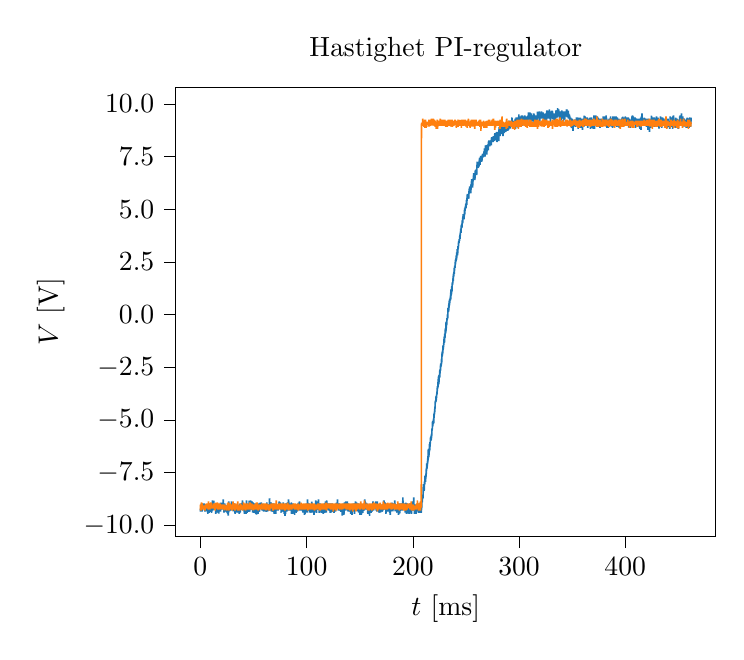
\begin{tikzpicture}

\definecolor{darkgray176}{RGB}{176,176,176}
\definecolor{darkorange25512714}{RGB}{255,127,14}
\definecolor{steelblue31119180}{RGB}{31,119,180}

\begin{axis}[
tick align=outside,
tick pos=left,
title={Hastighet PI-regulator},
x grid style={darkgray176},
xlabel={\(\displaystyle t\) [ms]},
xmin=-23.09538, xmax=485.00298,
xtick style={color=black},
xtick={-100,0,100,200,300,400,500},
xticklabels={
  \(\displaystyle {\ensuremath{-}100}\),
  \(\displaystyle {0}\),
  \(\displaystyle {100}\),
  \(\displaystyle {200}\),
  \(\displaystyle {300}\),
  \(\displaystyle {400}\),
  \(\displaystyle {500}\)
},
y grid style={darkgray176},
ylabel={\(\displaystyle V\) [V]},
ymin=-10.512697, ymax=10.756837,
ytick style={color=black},
ytick={-12.5,-10,-7.5,-5,-2.5,0,2.5,5,7.5,10,12.5},
yticklabels={
  \(\displaystyle {\ensuremath{-}12.5}\),
  \(\displaystyle {\ensuremath{-}10.0}\),
  \(\displaystyle {\ensuremath{-}7.5}\),
  \(\displaystyle {\ensuremath{-}5.0}\),
  \(\displaystyle {\ensuremath{-}2.5}\),
  \(\displaystyle {0.0}\),
  \(\displaystyle {2.5}\),
  \(\displaystyle {5.0}\),
  \(\displaystyle {7.5}\),
  \(\displaystyle {10.0}\),
  \(\displaystyle {12.5}\)
}
]
\addplot [semithick, steelblue31119180]
table {%
0 -9.2041
0.0923999999997704 -9.35059
0.184799999999985 -9.2041
0.277199999999755 -9.30176
0.36959999999997 -9.30176
0.46199999999974 -9.30176
0.554399999999955 -9.15527
0.646799999999725 -9.2041
0.73919999999994 -9.2041
0.83159999999971 -9.15527
0.923999999999925 -9.10645
1.0163999999997 -8.95996
1.10879999999991 -9.00879
1.20119999999968 -9.2041
1.29359999999989 -9.25293
1.38599999999967 -9.05762
1.47839999999988 -9.25293
1.57079999999965 -9.35059
1.66319999999986 -9.25293
1.75559999999964 -9.10645
1.84799999999985 -9.2041
1.94039999999962 -9.2041
2.03279999999983 -9.30176
2.12519999999961 -9.2041
2.21759999999982 -9.10645
2.30999999999959 -9.05762
2.4023999999998 -9.10645
2.49479999999958 -9.00879
2.58719999999979 -9.10645
2.6796 -9.10645
2.77199999999977 -8.95996
2.86439999999999 -9.15527
2.95679999999976 -9.05762
3.04919999999997 -9.10645
3.14159999999974 -9.10645
3.23399999999996 -9.15527
3.32639999999973 -9.15527
3.41879999999994 -9.10645
3.51119999999971 -9.00879
3.60359999999993 -9.00879
3.6959999999997 -8.95996
3.78839999999991 -9.15527
3.88079999999968 -9.05762
3.9731999999999 -9.10645
4.06559999999967 -9.15527
4.15799999999988 -9.10645
4.25039999999965 -9.35059
4.34279999999987 -9.2041
4.43519999999964 -9.25293
4.52759999999985 -9.2041
4.61999999999962 -9.05762
4.71239999999984 -9.10645
4.80479999999961 -9.10645
4.89719999999982 -9.00879
4.98959999999959 -9.05762
5.08199999999981 -9.2041
5.17439999999958 -9.15527
5.26679999999979 -9.10645
5.35920000000001 -9.25293
5.45159999999978 -9.30176
5.54399999999999 -9.30176
5.63639999999976 -9.10645
5.72879999999998 -9.25293
5.82119999999975 -9.30176
5.91359999999996 -9.10645
6.00599999999973 -9.05762
6.09839999999995 -9.15527
6.19079999999972 -9.05762
6.28319999999993 -9.10645
6.3755999999997 -9.2041
6.46799999999992 -9.05762
6.56039999999969 -9.2041
6.6527999999999 -9.25293
6.74519999999967 -9.30176
6.83759999999989 -9.39941
6.92999999999966 -9.30176
7.02239999999987 -9.44824
7.11479999999964 -9.30176
7.20719999999986 -9.15527
7.29959999999963 -9.10645
7.39199999999984 -9.25293
7.48439999999961 -9.05762
7.57679999999983 -9.15527
7.6691999999996 -9.25293
7.76159999999981 -9.30176
7.85399999999958 -9.39941
7.9463999999998 -9.15527
8.03880000000001 -9.30176
8.13119999999978 -9.39941
8.2236 -9.35059
8.31599999999977 -9.25293
8.40839999999998 -9.2041
8.50079999999975 -9.30176
8.59319999999997 -9.30176
8.68559999999974 -8.95996
8.77799999999995 -9.05762
8.87039999999972 -9.00879
8.96279999999994 -9.2041
9.05519999999971 -9.15527
9.14759999999992 -9.30176
9.23999999999969 -9.30176
9.33239999999991 -9.25293
9.42479999999968 -9.25293
9.51719999999989 -9.30176
9.60959999999966 -9.15527
9.70199999999988 -9.30176
9.79439999999965 -9.35059
9.88679999999986 -9.2041
9.97919999999963 -9.05762
10.0715999999998 -9.10645
10.1639999999996 -9.10645
10.2563999999998 -9.30176
10.3487999999996 -9.2041
10.4411999999998 -9.30176
10.5335999999996 -9.39941
10.6259999999998 -9.2041
10.7184 -9.35059
10.8107999999998 -9.15527
10.9032 -8.95996
10.9955999999998 -9.10645
11.088 -9.15527
11.1803999999998 -9.10645
11.2728 -8.81348
11.3651999999997 -8.95996
11.4576 -8.95996
11.5499999999997 -9.05762
11.6423999999999 -9.10645
11.7347999999997 -9.30176
11.8271999999999 -9.15527
11.9195999999997 -9.2041
12.0119999999999 -9.05762
12.1043999999997 -9.00879
12.1967999999999 -9.10645
12.2891999999997 -9.15527
12.3815999999999 -9.10645
12.4739999999997 -8.95996
12.5663999999999 -8.8623
12.6587999999996 -8.8623
12.7511999999999 -9.10645
12.8435999999996 -9.10645
12.9359999999998 -9.10645
13.0283999999996 -9.15527
13.1207999999998 -9.15527
13.2131999999996 -9.25293
13.3055999999998 -9.2041
13.3979999999996 -9.2041
13.4903999999998 -9.2041
13.5828 -9.05762
13.6751999999998 -9.25293
13.7676 -9.10645
13.8599999999998 -9.10645
13.9524 -9.10645
14.0447999999997 -9.10645
14.1372 -9.2041
14.2295999999997 -9.15527
14.3219999999999 -9.2041
14.4143999999997 -9.44824
14.5067999999999 -9.15527
14.5991999999997 -9.05762
14.6915999999999 -9.2041
14.7839999999997 -9.39941
14.8763999999999 -9.2041
14.9687999999997 -9.2041
15.0611999999999 -9.25293
15.1535999999997 -9.15527
15.2459999999999 -8.95996
15.3383999999996 -9.10645
15.4307999999999 -9.30176
15.5231999999996 -9.10645
15.6155999999998 -9.2041
15.7079999999996 -9.30176
15.8003999999998 -9.30176
15.8927999999996 -9.2041
15.9851999999998 -9.35059
16.0775999999996 -9.35059
16.1699999999998 -9.35059
16.2624 -9.25293
16.3547999999998 -9.15527
16.4472 -9.10645
16.5395999999998 -9.2041
16.632 -9.30176
16.7243999999998 -9.35059
16.8168 -9.10645
16.9091999999997 -9.30176
17.0016 -9.35059
17.0939999999997 -9.39941
17.1863999999999 -9.30176
17.2787999999997 -9.39941
17.3711999999999 -9.39941
17.4635999999997 -9.30176
17.5559999999999 -9.00879
17.6483999999997 -9.25293
17.7407999999999 -9.05762
17.8331999999997 -9.00879
17.9255999999999 -9.25293
18.0179999999996 -9.10645
18.1103999999999 -9.2041
18.2027999999996 -9.25293
18.2951999999998 -9.30176
18.3875999999996 -9.2041
18.4799999999998 -9.25293
18.5723999999996 -9.25293
18.6647999999998 -9.2041
18.7571999999996 -9.10645
18.8495999999998 -9.35059
18.942 -8.95996
19.0343999999998 -8.95996
19.1268 -9.25293
19.2191999999998 -9.2041
19.3116 -9.00879
19.4039999999998 -9.2041
19.4964 -9.25293
19.5887999999997 -9.10645
19.6812 -9.2041
19.7735999999997 -9.25293
19.8659999999999 -9.2041
19.9583999999997 -9.25293
20.0507999999999 -9.05762
20.1431999999997 -9.15527
20.2355999999999 -9.10645
20.3279999999997 -9.10645
20.4203999999999 -9.15527
20.5127999999997 -9.00879
20.6051999999999 -8.95996
20.6975999999996 -8.95996
20.7899999999999 -9.10645
20.8823999999996 -8.95996
20.9747999999998 -9.2041
21.0671999999996 -9.2041
21.1595999999998 -9.00879
21.2519999999996 -9.00879
21.3443999999998 -9.15527
21.4367999999996 -8.91113
21.5291999999998 -8.76465
21.6216 -8.91113
21.7139999999998 -9.10645
21.8064 -9.15527
21.8987999999998 -9.25293
21.9912 -9.15527
22.0835999999998 -9.25293
22.176 -9.2041
22.2683999999997 -9.39941
22.3608 -9.2041
22.4531999999997 -9.2041
22.5455999999999 -9.15527
22.6379999999997 -9.05762
22.7303999999999 -9.25293
22.8227999999997 -8.95996
22.9151999999999 -9.00879
23.0075999999997 -9.2041
23.0999999999999 -9.05762
23.1923999999997 -9.15527
23.2847999999999 -9.30176
23.3771999999997 -9.30176
23.4695999999999 -9.35059
23.5619999999996 -9.05762
23.6543999999999 -9.2041
23.7467999999996 -9.30176
23.8391999999998 -9.2041
23.9315999999996 -9.05762
24.0239999999998 -9.15527
24.1163999999996 -9.25293
24.2087999999998 -9.15527
24.3011999999996 -9.10645
24.3935999999998 -9.30176
24.486 -9.30176
24.5783999999998 -9.25293
24.6708 -9.2041
24.7631999999998 -9.35059
24.8556 -9.35059
24.9479999999997 -9.35059
25.0404 -9.30176
25.1327999999997 -9.2041
25.2251999999999 -9.2041
25.3175999999997 -9.25293
25.4099999999999 -9.2041
25.5023999999997 -9.05762
25.5947999999999 -9.2041
25.6871999999997 -9.44824
25.7795999999999 -9.2041
25.8719999999997 -9.39941
25.9643999999999 -9.30176
26.0567999999997 -9.25293
26.1491999999999 -9.49707
26.2415999999996 -9.49707
26.3339999999999 -9.35059
26.4263999999996 -9.39941
26.5187999999998 -9.05762
26.6111999999996 -8.8623
26.7035999999998 -8.95996
26.7959999999996 -9.05762
26.8883999999998 -9.2041
26.9807999999996 -9.25293
27.0731999999998 -9.10645
27.1656 -9.2041
27.2579999999998 -9.30176
27.3504 -9.25293
27.4427999999998 -9.30176
27.5352 -9.30176
27.6275999999998 -9.10645
27.72 -9.15527
27.8123999999997 -9.25293
27.9048 -9.15527
27.9971999999997 -9.10645
28.0895999999999 -9.10645
28.1819999999997 -9.00879
28.2743999999999 -9.10645
28.3667999999997 -9.30176
28.4591999999999 -9.2041
28.5515999999997 -9.2041
28.6439999999999 -9.30176
28.7363999999997 -9.10645
28.8287999999999 -9.15527
28.9211999999996 -9.2041
29.0135999999999 -9.2041
29.1059999999996 -9.05762
29.1983999999998 -9.00879
29.2907999999996 -8.8623
29.3831999999998 -9.05762
29.4755999999996 -9.00879
29.5679999999998 -9.00879
29.6603999999996 -8.95996
29.7527999999998 -9.2041
29.8452 -9.10645
29.9375999999998 -9.05762
30.03 -9.10645
30.1223999999998 -9.10645
30.2148 -9.05762
30.3071999999998 -8.95996
30.3996 -9.00879
30.4919999999997 -9.00879
30.5844 -8.91113
30.6767999999997 -9.10645
30.7691999999999 -9.10645
30.8615999999997 -9.00879
30.9539999999999 -9.30176
31.0463999999997 -9.30176
31.1387999999999 -9.30176
31.2311999999997 -9.25293
31.3235999999999 -9.25293
31.4159999999997 -9.15527
31.5083999999999 -9.15527
31.6007999999997 -9.25293
31.6931999999999 -9.10645
31.7855999999996 -9.10645
31.8779999999999 -8.95996
31.9703999999996 -9.2041
32.0627999999998 -9.10645
32.1551999999996 -9.25293
32.2475999999998 -9.25293
32.3399999999996 -9.2041
32.4323999999998 -9.39941
32.5247999999996 -9.30176
32.6171999999998 -9.39941
32.7096 -9.44824
32.8019999999998 -9.30176
32.8944 -9.25293
32.9867999999998 -9.05762
33.0792 -9.10645
33.1715999999997 -9.10645
33.264 -9.2041
33.3563999999997 -9.2041
33.4487999999999 -9.35059
33.5411999999997 -9.15527
33.6335999999999 -9.35059
33.7259999999997 -9.30176
33.8183999999999 -9.2041
33.9107999999997 -9.30176
34.0031999999999 -9.15527
34.0955999999997 -9.30176
34.1879999999999 -9.2041
34.2803999999997 -9.05762
34.3727999999999 -9.05762
34.4651999999996 -9.30176
34.5575999999999 -9.2041
34.6499999999996 -9.25293
34.7423999999998 -9.25293
34.8347999999996 -9.39941
34.9271999999998 -9.2041
35.0195999999996 -9.30176
35.1119999999998 -9.25293
35.2043999999996 -9.30176
35.2967999999998 -9.30176
35.3892 -9.2041
35.4815999999998 -9.2041
35.574 -9.25293
35.6663999999998 -9.10645
35.7588 -9.15527
35.8511999999997 -9.2041
35.9436 -9.05762
36.0359999999997 -9.10645
36.1283999999999 -9.30176
36.2207999999997 -9.2041
36.3131999999999 -9.10645
36.4055999999997 -9.2041
36.4979999999999 -9.44824
36.5903999999997 -9.05762
36.6827999999999 -9.15527
36.7751999999997 -9.15527
36.8675999999999 -9.00879
36.9599999999997 -9.00879
37.0523999999999 -9.10645
37.1447999999996 -9.15527
37.2371999999999 -9.10645
37.3295999999996 -9.25293
37.4219999999998 -9.39941
37.5143999999996 -9.2041
37.6067999999998 -9.35059
37.6991999999996 -9.2041
37.7915999999998 -9.30176
37.8839999999996 -9.10645
37.9763999999998 -9.10645
38.0688 -9.2041
38.1611999999998 -9.05762
38.2536 -9.00879
38.3459999999998 -9.00879
38.4384 -9.05762
38.5307999999998 -8.95996
38.6232 -9.05762
38.7155999999997 -9.10645
38.808 -9.25293
38.9003999999997 -9.10645
38.9927999999999 -9.10645
39.0851999999997 -9.00879
39.1775999999999 -9.10645
39.2699999999997 -8.95996
39.3623999999999 -8.95996
39.4547999999997 -8.95996
39.5471999999999 -8.81348
39.6395999999997 -9.10645
39.7319999999999 -9.10645
39.8243999999996 -9.10645
39.9167999999999 -9.2041
40.0091999999996 -9.25293
40.1015999999998 -9.25293
40.1939999999996 -9.25293
40.2863999999998 -9.25293
40.3787999999996 -9.25293
40.4711999999998 -9.2041
40.5635999999996 -9.00879
40.6559999999998 -9.10645
40.7484 -9.05762
40.8407999999998 -9.05762
40.9332 -9.10645
41.0255999999998 -9.10645
41.118 -9.10645
41.2103999999998 -9.35059
41.3028 -9.30176
41.3951999999997 -9.44824
41.4876 -9.2041
41.5799999999997 -9.39941
41.6723999999999 -9.15527
41.7647999999997 -9.05762
41.8571999999999 -9.10645
41.9495999999997 -9.25293
42.0419999999999 -9.10645
42.1343999999997 -9.15527
42.2267999999999 -9.2041
42.3191999999997 -9.30176
42.4115999999999 -9.35059
42.5039999999996 -9.15527
42.5963999999999 -9.25293
42.6887999999996 -9.25293
42.7811999999999 -9.30176
42.8735999999996 -9.30176
42.9659999999998 -9.44824
43.0583999999996 -9.25293
43.1507999999998 -9.2041
43.2431999999996 -9.00879
43.3355999999998 -8.81348
43.4279999999996 -8.95996
43.5203999999998 -9.10645
43.6128 -9.2041
43.7051999999998 -9.30176
43.7976 -9.39941
43.8899999999998 -9.30176
43.9824 -9.35059
44.0747999999997 -9.30176
44.1672 -9.25293
44.2595999999997 -9.2041
44.3519999999999 -9.35059
44.4443999999997 -9.10645
44.5367999999999 -9.00879
44.6291999999997 -9.00879
44.7215999999999 -9.05762
44.8139999999997 -9.05762
44.9063999999999 -9.15527
44.9987999999997 -9.25293
45.0911999999999 -9.25293
45.1835999999997 -9.30176
45.2759999999999 -9.35059
45.3683999999996 -9.30176
45.4607999999999 -9.05762
45.5531999999996 -9.2041
45.6455999999998 -9.25293
45.7379999999996 -9.10645
45.8303999999998 -9.00879
45.9227999999996 -8.8623
46.0151999999998 -8.8623
46.1075999999996 -9.10645
46.1999999999998 -9.2041
46.2924 -9.30176
46.3847999999998 -9.35059
46.4772 -9.15527
46.5695999999998 -9.10645
46.662 -9.15527
46.7543999999997 -9.15527
46.8468 -9.2041
46.9391999999997 -9.10645
47.0316 -9.15527
47.1239999999997 -9.05762
47.2163999999999 -8.95996
47.3087999999997 -8.81348
47.4011999999999 -9.00879
47.4935999999997 -9.10645
47.5859999999999 -9.10645
47.6783999999997 -9.25293
47.7707999999999 -9.00879
47.8631999999997 -9.10645
47.9555999999999 -9.10645
48.0479999999996 -9.05762
48.1403999999999 -9.2041
48.2327999999996 -9.15527
48.3251999999998 -9.05762
48.4175999999996 -8.91113
48.5099999999998 -8.8623
48.6023999999996 -9.10645
48.6947999999998 -9.10645
48.7871999999996 -9.15527
48.8795999999998 -9.10645
48.972 -9.2041
49.0643999999998 -9.15527
49.1568 -9.39941
49.2491999999998 -9.15527
49.3416 -9.30176
49.4339999999998 -9.30176
49.5264 -9.30176
49.6187999999997 -8.91113
49.7112 -8.95996
49.8035999999997 -9.10645
49.8959999999999 -9.15527
49.9883999999997 -9.10645
50.0807999999999 -9.15527
50.1731999999997 -9.05762
50.2655999999999 -9.30176
50.3579999999997 -9.39941
50.4503999999999 -9.15527
50.5427999999997 -9.30176
50.6351999999999 -9.35059
50.7275999999997 -9.30176
50.8199999999999 -9.25293
50.9123999999996 -9.30176
51.0047999999998 -9.15527
51.0971999999996 -9.30176
51.1895999999998 -8.95996
51.2819999999996 -9.10645
51.3743999999998 -9.25293
51.4667999999996 -9.35059
51.5591999999998 -9.39941
51.6515999999996 -9.15527
51.7439999999998 -9.2041
51.8364 -9.35059
51.9287999999998 -9.25293
52.0212 -9.44824
52.1135999999998 -9.2041
52.206 -9.05762
52.2983999999997 -9.15527
52.3908 -9.30176
52.4831999999997 -9.15527
52.5755999999999 -9.25293
52.6679999999997 -9.25293
52.7603999999999 -9.30176
52.8527999999997 -9.44824
52.9451999999999 -9.44824
53.0375999999997 -9.30176
53.1299999999999 -9.35059
53.2223999999997 -9.30176
53.3147999999999 -9.30176
53.4071999999997 -9.39941
53.4995999999999 -9.00879
53.5919999999996 -9.2041
53.6843999999999 -9.05762
53.7767999999996 -9.25293
53.8691999999998 -9.2041
53.9615999999996 -9.30176
54.0539999999998 -9.15527
54.1463999999996 -9.15527
54.2387999999998 -9.44824
54.3311999999996 -9.05762
54.4235999999998 -9.30176
54.516 -9.10645
54.6083999999998 -9.25293
54.7008 -9.00879
54.7931999999998 -8.95996
54.8856 -9.10645
54.9779999999998 -9.15527
55.0704 -9.05762
55.1627999999997 -9.30176
55.2551999999999 -9.30176
55.3475999999997 -9.35059
55.4399999999999 -9.00879
55.5323999999997 -9.30176
55.6247999999999 -9.35059
55.7171999999997 -9.25293
55.8095999999999 -9.10645
55.9019999999997 -9.10645
55.9943999999999 -9.05762
56.0867999999997 -9.00879
56.1791999999999 -8.95996
56.2715999999996 -8.95996
56.3639999999999 -8.95996
56.4563999999996 -9.10645
56.5487999999998 -9.10645
56.6411999999996 -9.10645
56.7335999999998 -9.10645
56.8259999999996 -9.10645
56.9183999999998 -9.00879
57.0107999999996 -9.00879
57.1031999999998 -9.10645
57.1956 -9.10645
57.2879999999998 -9.00879
57.3804 -8.91113
57.4727999999998 -9.10645
57.5652 -9.00879
57.6575999999998 -9.10645
57.75 -9.10645
57.8423999999997 -9.15527
57.9348 -9.25293
58.0271999999997 -9.2041
58.1195999999999 -9.30176
58.2119999999997 -9.10645
58.3043999999999 -9.2041
58.3967999999997 -9.25293
58.4891999999999 -9.10645
58.5815999999997 -9.10645
58.6739999999999 -9.15527
58.7663999999997 -9.00879
58.8587999999999 -9.00879
58.9511999999996 -9.15527
59.0435999999999 -9.15527
59.1359999999996 -9.10645
59.2283999999999 -9.25293
59.3207999999996 -9.30176
59.4131999999998 -9.30176
59.5055999999996 -9.2041
59.5979999999998 -9.30176
59.6903999999996 -9.2041
59.7827999999998 -9.35059
59.8752 -9.15527
59.9675999999998 -9.00879
60.06 -9.05762
60.1523999999998 -9.05762
60.2448 -9.15527
60.3371999999998 -9.30176
60.4296 -9.30176
60.5219999999997 -9.30176
60.6144 -9.25293
60.7067999999997 -9.30176
60.7991999999999 -9.30176
60.8915999999997 -9.25293
60.9839999999999 -9.15527
61.0763999999997 -9.30176
61.1687999999999 -9.25293
61.2611999999997 -9.15527
61.3535999999999 -9.10645
61.4459999999997 -9.2041
61.5383999999999 -9.15527
61.6307999999997 -9.30176
61.7231999999999 -9.25293
61.8155999999996 -9.35059
61.9079999999999 -9.30176
62.0003999999996 -9.30176
62.0927999999998 -9.25293
62.1851999999996 -9.30176
62.2775999999998 -9.35059
62.3699999999996 -9.30176
62.4623999999998 -9.10645
62.5547999999996 -8.91113
62.6471999999998 -9.10645
62.7396 -9.10645
62.8319999999998 -9.25293
62.9244 -9.05762
63.0167999999998 -9.15527
63.1092 -9.30176
63.2015999999997 -9.25293
63.294 -9.30176
63.3863999999997 -9.30176
63.4787999999999 -9.25293
63.5711999999997 -9.2041
63.6635999999999 -9.10645
63.7559999999997 -9.15527
63.8483999999999 -9.00879
63.9407999999997 -9.10645
64.0331999999999 -9.30176
64.1255999999997 -9.15527
64.2179999999999 -9.30176
64.3103999999997 -9.2041
64.4027999999999 -9.30176
64.4951999999996 -9.15527
64.5875999999999 -9.30176
64.6799999999996 -9.2041
64.7723999999998 -9.30176
64.8647999999996 -9.15527
64.9571999999998 -8.95996
65.0495999999996 -8.71582
65.1419999999998 -8.76465
65.2343999999996 -8.95996
65.3267999999998 -8.95996
65.4192 -9.10645
65.5115999999998 -9.00879
65.604 -9.15527
65.6963999999998 -9.30176
65.7888 -9.2041
65.8811999999998 -9.15527
65.9736 -9.15527
66.0659999999997 -9.00879
66.1583999999999 -9.10645
66.2507999999997 -8.95996
66.3431999999999 -9.15527
66.4355999999997 -9.05762
66.5279999999999 -8.91113
66.6203999999997 -9.15527
66.7127999999999 -9.25293
66.8051999999997 -9.2041
66.8975999999999 -9.25293
66.9899999999997 -9.35059
67.0823999999999 -9.2041
67.1747999999996 -9.25293
67.2671999999999 -9.2041
67.3595999999996 -9.30176
67.4519999999998 -9.25293
67.5443999999996 -9.10645
67.6367999999998 -9.05762
67.7291999999996 -8.95996
67.8215999999998 -9.25293
67.9139999999996 -9.00879
68.0063999999998 -9.15527
68.0988 -9.30176
68.1911999999998 -9.30176
68.2836 -9.30176
68.3759999999998 -9.2041
68.4684 -9.30176
68.5607999999998 -9.35059
68.6532 -9.25293
68.7455999999997 -9.2041
68.838 -9.15527
68.9303999999997 -9.2041
69.0227999999999 -9.05762
69.1151999999997 -8.95996
69.2075999999999 -9.10645
69.2999999999997 -9.35059
69.3923999999999 -9.39941
69.4847999999997 -9.44824
69.5771999999999 -9.39941
69.6695999999997 -9.25293
69.7619999999999 -9.30176
69.8543999999997 -9.30176
69.9467999999999 -9.00879
70.0391999999996 -9.2041
70.1315999999998 -9.10645
70.2239999999996 -9.00879
70.3163999999998 -9.10645
70.4087999999996 -9.2041
70.5011999999998 -9.10645
70.5935999999996 -9.2041
70.6859999999998 -9.35059
70.7783999999996 -9.39941
70.8707999999998 -9.30176
70.9632 -9.44824
71.0555999999998 -9.30176
71.148 -9.25293
71.2403999999998 -9.05762
71.3328 -9.25293
71.4251999999997 -9.00879
71.5176 -9.05762
71.6099999999997 -9.00879
71.7023999999999 -9.25293
71.7947999999997 -9.25293
71.8871999999999 -9.2041
71.9795999999997 -9.15527
72.0719999999999 -9.2041
72.1643999999997 -9.15527
72.2567999999999 -9.15527
72.3491999999997 -9.30176
72.4415999999999 -9.10645
72.5339999999997 -9.30176
72.6263999999999 -9.15527
72.7187999999996 -9.00879
72.8111999999999 -9.10645
72.9035999999996 -9.00879
72.9959999999998 -9.25293
73.0883999999996 -9.30176
73.1807999999998 -9.2041
73.2731999999996 -9.05762
73.3655999999998 -9.2041
73.4579999999996 -9.2041
73.5503999999998 -9.15527
73.6428 -9.10645
73.7351999999998 -9.15527
73.8276 -9.15527
73.9199999999998 -8.95996
74.0124 -8.95996
74.1047999999998 -8.95996
74.1972 -8.8623
74.2895999999997 -9.00879
74.3819999999999 -9.00879
74.4743999999997 -8.95996
74.5667999999999 -9.10645
74.6591999999997 -9.00879
74.7515999999999 -9.10645
74.8439999999997 -8.95996
74.9363999999999 -9.10645
75.0287999999997 -9.05762
75.1211999999999 -8.95996
75.2135999999997 -9.05762
75.3059999999999 -8.91113
75.3983999999996 -9.00879
75.4907999999999 -9.00879
75.5831999999996 -9.10645
75.6755999999998 -9.10645
75.7679999999996 -9.10645
75.8603999999998 -9.25293
75.9527999999996 -9.15527
76.0451999999998 -9.25293
76.1375999999996 -9.39941
76.2299999999998 -9.2041
76.3224 -9.10645
76.4147999999998 -9.10645
76.5072 -9.10645
76.5995999999998 -9.05762
76.692 -9.10645
76.7843999999997 -9.15527
76.8768 -9.15527
76.9691999999997 -9.15527
77.0616 -9.25293
77.1539999999997 -9.30176
77.2463999999999 -9.35059
77.3387999999997 -9.10645
77.4311999999999 -9.30176
77.5235999999997 -9.25293
77.6159999999999 -9.35059
77.7083999999997 -9.15527
77.8007999999999 -9.15527
77.8931999999997 -9.2041
77.9855999999999 -8.91113
78.0779999999996 -9.25293
78.1703999999999 -9.2041
78.2627999999996 -9.25293
78.3551999999999 -9.15527
78.4475999999996 -9.30176
78.5399999999998 -9.30176
78.6323999999996 -9.35059
78.7247999999998 -9.2041
78.8171999999996 -9.44824
78.9095999999998 -9.25293
79.002 -9.15527
79.0943999999998 -9.10645
79.1868 -9.2041
79.2791999999998 -9.00879
79.3716 -9.30176
79.4639999999998 -9.25293
79.5564 -9.30176
79.6487999999997 -9.5459
79.7412 -9.30176
79.8335999999997 -9.39941
79.9259999999999 -9.25293
80.0183999999997 -9.35059
80.1107999999999 -9.44824
80.2031999999997 -9.25293
80.2955999999999 -9.30176
80.3879999999997 -8.95996
80.4803999999999 -9.10645
80.5727999999997 -9.05762
80.6651999999999 -9.25293
80.7575999999997 -9.25293
80.8499999999999 -9.25293
80.9423999999996 -9.2041
81.0347999999998 -9.30176
81.1271999999996 -9.25293
81.2195999999998 -9.2041
81.3119999999996 -9.35059
81.4043999999998 -9.2041
81.4967999999996 -9.15527
81.5891999999998 -9.2041
81.6815999999996 -9.25293
81.7739999999998 -9.00879
81.8664 -8.91113
81.9587999999998 -9.15527
82.0512 -9.10645
82.1435999999998 -9.30176
82.236 -9.2041
82.3283999999997 -9.25293
82.4208 -9.10645
82.5131999999997 -9.2041
82.6056 -9.15527
82.6979999999997 -9.30176
82.7903999999999 -9.05762
82.8827999999997 -9.10645
82.9751999999999 -8.76465
83.0675999999997 -8.95996
83.1599999999999 -8.91113
83.2523999999997 -8.91113
83.3447999999999 -8.95996
83.4371999999996 -9.15527
83.5295999999999 -9.15527
83.6219999999996 -9.00879
83.7143999999999 -9.00879
83.8067999999996 -9.30176
83.8991999999998 -9.2041
83.9915999999996 -9.10645
84.0839999999998 -8.95996
84.1763999999996 -9.10645
84.2687999999998 -9.10645
84.3611999999996 -9.00879
84.4535999999998 -8.95996
84.546 -9.15527
84.6383999999998 -9.2041
84.7308 -9.15527
84.8231999999998 -9.2041
84.9156 -9.00879
85.0079999999998 -9.25293
85.1004 -9.25293
85.1927999999997 -9.15527
85.2851999999999 -9.15527
85.3775999999997 -9.15527
85.4699999999999 -9.05762
85.5623999999997 -9.05762
85.6547999999999 -8.91113
85.7471999999997 -9.15527
85.8395999999999 -9.44824
85.9319999999997 -9.35059
86.0243999999999 -9.15527
86.1167999999997 -9.25293
86.2091999999999 -9.25293
86.3015999999996 -9.15527
86.3939999999999 -9.44824
86.4863999999996 -9.35059
86.5787999999998 -9.30176
86.6711999999996 -9.30176
86.7635999999998 -9.30176
86.8559999999996 -9.15527
86.9483999999998 -8.95996
87.0407999999996 -9.00879
87.1331999999998 -9.10645
87.2256 -9.25293
87.3179999999998 -9.30176
87.4104 -9.25293
87.5027999999998 -9.35059
87.5952 -9.30176
87.6875999999997 -9.05762
87.78 -9.15527
87.8723999999997 -9.15527
87.9648 -9.25293
88.0571999999997 -9.15527
88.1495999999999 -9.00879
88.2419999999997 -9.15527
88.3343999999999 -9.25293
88.4267999999997 -9.44824
88.5191999999999 -9.15527
88.6115999999997 -9.30176
88.7039999999999 -9.49707
88.7963999999997 -9.15527
88.8887999999999 -9.2041
88.9811999999996 -9.30176
89.0735999999999 -9.30176
89.1659999999996 -9.30176
89.2583999999999 -9.25293
89.3507999999996 -9.2041
89.4431999999998 -9.15527
89.5355999999996 -9.00879
89.6279999999998 -9.10645
89.7203999999996 -9.15527
89.8127999999998 -9.10645
89.9052 -9.30176
89.9975999999998 -9.15527
90.09 -9.39941
90.1823999999998 -9.30176
90.2748 -9.30176
90.3671999999998 -9.15527
90.4596 -9.15527
90.5519999999997 -9.10645
90.6444 -9.10645
90.7367999999997 -9.00879
90.8291999999999 -9.05762
90.9215999999997 -9.05762
91.0139999999999 -9.30176
91.1063999999997 -9.25293
91.1987999999999 -9.2041
91.2911999999997 -9.35059
91.3835999999999 -9.25293
91.4759999999997 -9.25293
91.5683999999999 -9.2041
91.6607999999997 -9.25293
91.7531999999999 -9.10645
91.8455999999996 -9.15527
91.9379999999998 -9.05762
92.0303999999996 -8.95996
92.1227999999998 -9.05762
92.2151999999996 -9.05762
92.3075999999998 -8.95996
92.3999999999996 -8.95996
92.4923999999998 -9.10645
92.5847999999996 -9.10645
92.6771999999998 -9.00879
92.7696 -9.00879
92.8619999999998 -9.00879
92.9544 -9.05762
93.0467999999998 -9.00879
93.1392 -9.00879
93.2315999999997 -8.8623
93.324 -8.95996
93.4163999999997 -8.95996
93.5088 -8.95996
93.6011999999997 -9.10645
93.6935999999999 -9.10645
93.7859999999997 -9.30176
93.8783999999999 -9.2041
93.9707999999997 -9.10645
94.0631999999999 -9.25293
94.1555999999997 -9.2041
94.2479999999999 -9.25293
94.3403999999997 -9.25293
94.4327999999999 -9.2041
94.5251999999996 -9.15527
94.6175999999999 -9.00879
94.7099999999996 -9.05762
94.8023999999998 -9.2041
94.8947999999996 -9.2041
94.9871999999998 -9.2041
95.0795999999996 -9.05762
95.1719999999998 -9.25293
95.2643999999996 -9.30176
95.3567999999998 -9.2041
95.4492 -9.30176
95.5415999999998 -9.25293
95.634 -9.30176
95.7263999999998 -9.05762
95.8188 -9.05762
95.9111999999998 -9.00879
96.0036 -9.2041
96.0959999999997 -9.25293
96.1883999999999 -9.10645
96.2807999999997 -9.35059
96.3731999999999 -9.30176
96.4655999999997 -9.2041
96.5579999999999 -9.35059
96.6503999999997 -9.35059
96.7427999999999 -9.25293
96.8351999999997 -9.35059
96.9275999999999 -9.25293
97.0199999999997 -9.25293
97.1123999999999 -9.2041
97.2047999999997 -9.10645
97.2971999999999 -9.10645
97.3895999999996 -9.25293
97.4819999999998 -9.30176
97.5743999999996 -9.35059
97.6667999999998 -9.30176
97.7591999999996 -9.35059
97.8515999999998 -9.30176
97.9439999999996 -9.49707
98.0363999999998 -9.30176
98.1288 -9.2041
98.2211999999998 -9.25293
98.3136 -9.05762
98.4059999999998 -9.10645
98.4984 -9.30176
98.5907999999998 -9.44824
98.6832 -9.15527
98.7755999999997 -9.30176
98.868 -9.25293
98.9603999999997 -9.30176
99.0527999999999 -9.2041
99.1451999999997 -9.25293
99.2375999999999 -9.15527
99.3299999999997 -9.30176
99.4223999999999 -9.25293
99.5147999999997 -9.15527
99.6071999999999 -9.15527
99.6995999999997 -9.00879
99.7919999999999 -9.00879
99.8843999999997 -9.15527
99.9767999999999 -9.25293
100.0692 -9.10645
100.1616 -9.30176
100.254 -9.2041
100.3464 -9.35059
100.4388 -9.35059
100.5312 -9.10645
100.6236 -9.00879
100.716 -9.15527
100.8084 -9.10645
100.9008 -8.76465
100.9932 -8.95996
101.0856 -8.95996
101.178 -8.95996
101.2704 -9.00879
101.3628 -8.95996
101.4552 -9.15527
101.5476 -9.15527
101.64 -9.10645
101.7324 -9.10645
101.8248 -9.00879
101.9172 -9.30176
102.0096 -8.95996
102.102 -9.10645
102.1944 -8.95996
102.2868 -9.05762
102.3792 -8.95996
102.4716 -9.10645
102.564 -9.10645
102.6564 -9.39941
102.7488 -9.05762
102.8412 -9.2041
102.9336 -9.2041
103.026 -9.15527
103.1184 -9.10645
103.2108 -9.2041
103.3032 -9.10645
103.3956 -9.25293
103.488 -9.10645
103.5804 -9.10645
103.6728 -9.2041
103.7652 -9.2041
103.8576 -9.25293
103.95 -9.15527
104.0424 -9.30176
104.1348 -9.30176
104.2272 -9.39941
104.3196 -9.15527
104.412 -9.2041
104.5044 -9.25293
104.5968 -9.2041
104.6892 -9.05762
104.7816 -9.25293
104.874 -8.91113
104.9664 -8.91113
105.0588 -9.10645
105.1512 -9.2041
105.2436 -9.30176
105.336 -9.2041
105.4284 -9.2041
105.5208 -9.35059
105.6132 -9.35059
105.7056 -9.10645
105.798 -9.30176
105.8904 -9.25293
105.9828 -9.00879
106.0752 -9.10645
106.1676 -9.30176
106.26 -9.10645
106.3524 -9.30176
106.4448 -9.30176
106.5372 -9.15527
106.6296 -9.39941
106.722 -9.35059
106.8144 -9.35059
106.9068 -9.49707
106.9992 -9.15527
107.0916 -9.44824
107.184 -9.15527
107.2764 -9.15527
107.3688 -9.10645
107.4612 -9.00879
107.5536 -9.25293
107.646 -9.15527
107.7384 -9.00879
107.8308 -9.30176
107.9232 -9.10645
108.0156 -9.10645
108.108 -9.2041
108.2004 -9.25293
108.2928 -9.25293
108.3852 -9.00879
108.4776 -9.05762
108.57 -9.10645
108.6624 -8.81348
108.7548 -9.05762
108.8472 -9.05762
108.9396 -9.15527
109.032 -9.35059
109.1244 -9.30176
109.2168 -9.2041
109.3092 -9.39941
109.4016 -9.35059
109.494 -9.2041
109.5864 -9.10645
109.6788 -9.10645
109.7712 -9.10645
109.8636 -9.15527
109.956 -9.10645
110.0484 -9.05762
110.1408 -8.95996
110.2332 -8.8623
110.3256 -9.10645
110.418 -9.10645
110.5104 -9.25293
110.6028 -9.00879
110.6952 -9.15527
110.7876 -9.05762
110.88 -9.00879
110.9724 -9.00879
111.0648 -9.10645
111.1572 -8.76465
111.2496 -8.95996
111.342 -9.00879
111.4344 -9.05762
111.5268 -9.15527
111.6192 -9.05762
111.7116 -9.05762
111.804 -9.30176
111.8964 -9.39941
111.9888 -9.30176
112.0812 -9.15527
112.1736 -9.39941
112.266 -9.30176
112.3584 -9.10645
112.4508 -9.00879
112.5432 -9.15527
112.6356 -8.95996
112.728 -9.10645
112.8204 -9.15527
112.9128 -9.15527
113.0052 -9.30176
113.0976 -9.35059
113.19 -9.15527
113.2824 -9.2041
113.3748 -9.25293
113.4672 -9.2041
113.5596 -9.30176
113.652 -9.25293
113.7444 -9.00879
113.8368 -9.10645
113.9292 -9.10645
114.0216 -9.10645
114.114 -9.30176
114.2064 -9.30176
114.2988 -9.39941
114.3912 -9.25293
114.4836 -9.30176
114.576 -9.30176
114.6684 -9.39941
114.7608 -9.25293
114.8532 -9.2041
114.9456 -9.15527
115.038 -9.00879
115.1304 -9.10645
115.2228 -9.15527
115.3152 -9.30176
115.4076 -9.35059
115.5 -9.10645
115.5924 -9.44824
115.6848 -9.2041
115.7772 -9.35059
115.8696 -9.30176
115.962 -9.30176
116.0544 -9.2041
116.1468 -9.30176
116.2392 -9.05762
116.3316 -9.10645
116.424 -9.00879
116.5164 -9.00879
116.6088 -9.25293
116.7012 -9.2041
116.7936 -9.39941
116.886 -9.30176
116.9784 -9.30176
117.0708 -9.30176
117.1632 -9.2041
117.2556 -9.05762
117.348 -9.2041
117.4404 -9.10645
117.5328 -9.10645
117.6252 -8.91113
117.7176 -8.8623
117.81 -9.05762
117.9024 -9.15527
117.9948 -9.10645
118.0872 -9.30176
118.1796 -9.30176
118.272 -9.35059
118.3644 -9.30176
118.4568 -9.35059
118.5492 -9.35059
118.6416 -9.2041
118.734 -9.25293
118.8264 -8.81348
118.9188 -8.8623
119.0112 -8.91113
119.1036 -9.00879
119.196 -8.95996
119.2884 -9.05762
119.3808 -8.95996
119.4732 -9.25293
119.5656 -9.10645
119.658 -9.15527
119.7504 -9.15527
119.8428 -9.10645
119.9352 -9.00879
120.0276 -8.95996
120.12 -9.05762
120.2124 -9.00879
120.3048 -8.95996
120.3972 -9.10645
120.4896 -8.95996
120.582 -9.00879
120.6744 -9.25293
120.7668 -9.30176
120.8592 -9.25293
120.9516 -9.30176
121.044 -9.10645
121.1364 -9.05762
121.2288 -9.2041
121.3212 -9.15527
121.4136 -9.00879
121.506 -8.95996
121.5984 -9.10645
121.6908 -9.15527
121.7832 -9.25293
121.8756 -9.2041
121.968 -9.2041
122.0604 -9.30176
122.1528 -9.39941
122.2452 -9.30176
122.3376 -9.2041
122.43 -9.15527
122.5224 -9.15527
122.6148 -9.15527
122.7072 -8.95996
122.7996 -9.25293
122.892 -9.2041
122.9844 -9.05762
123.0768 -9.15527
123.1692 -9.35059
123.2616 -9.35059
123.354 -9.25293
123.4464 -9.30176
123.5388 -9.25293
123.6312 -9.2041
123.7236 -9.30176
123.816 -9.15527
123.9084 -9.30176
124.0008 -8.95996
124.0932 -9.2041
124.1856 -9.15527
124.278 -9.2041
124.3704 -9.35059
124.4628 -9.30176
124.5552 -9.2041
124.6476 -9.25293
124.74 -9.30176
124.8324 -9.30176
124.9248 -9.15527
125.0172 -9.10645
125.1096 -9.15527
125.202 -9.00879
125.2944 -9.05762
125.3868 -9.10645
125.4792 -9.2041
125.5716 -9.10645
125.664 -9.10645
125.7564 -9.30176
125.8488 -9.39941
125.9412 -9.30176
126.0336 -9.00879
126.126 -9.30176
126.2184 -9.2041
126.3108 -9.05762
126.4032 -9.00879
126.4956 -9.05762
126.588 -9.10645
126.6804 -9.10645
126.7728 -9.00879
126.8652 -9.10645
126.9576 -9.15527
127.05 -9.10645
127.1424 -9.35059
127.2348 -9.15527
127.3272 -9.10645
127.4196 -9.10645
127.512 -9.15527
127.6044 -9.2041
127.6968 -9.10645
127.7892 -9.10645
127.8816 -9.00879
127.974 -8.95996
128.0664 -8.95996
128.1588 -9.00879
128.2512 -8.95996
128.3436 -9.15527
128.436 -9.00879
128.5284 -9.00879
128.6208 -9.00879
128.7132 -9.05762
128.8056 -9.10645
128.898 -9.10645
128.9904 -9.10645
129.0828 -8.76465
129.1752 -9.00879
129.2676 -9.00879
129.36 -8.95996
129.4524 -9.05762
129.5448 -9.15527
129.6372 -9.10645
129.7296 -9.2041
129.822 -9.10645
129.9144 -9.30176
130.0068 -9.10645
130.0992 -9.25293
130.1916 -9.10645
130.284 -9.2041
130.3764 -9.2041
130.4688 -9.15527
130.5612 -8.95996
130.6536 -9.10645
130.746 -9.15527
130.8384 -9.25293
130.9308 -9.10645
131.0232 -9.25293
131.1156 -9.30176
131.208 -9.05762
131.3004 -9.25293
131.3928 -9.25293
131.4852 -9.2041
131.5776 -9.25293
131.67 -9.10645
131.7624 -9.15527
131.8548 -9.25293
131.9472 -9.30176
132.0396 -9.30176
132.132 -9.10645
132.2244 -9.2041
132.3168 -9.30176
132.4092 -9.35059
132.5016 -9.30176
132.594 -9.30176
132.6864 -9.30176
132.7788 -9.30176
132.8712 -9.15527
132.9636 -9.10645
133.056 -9.15527
133.1484 -9.00879
133.2408 -9.15527
133.3332 -9.2041
133.4256 -9.30176
133.518 -9.49707
133.6104 -9.49707
133.7028 -9.49707
133.7952 -9.39941
133.8876 -9.30176
133.98 -9.35059
134.0724 -9.30176
134.1648 -9.00879
134.2572 -9.00879
134.3496 -9.00879
134.442 -9.00879
134.5344 -9.15527
134.6268 -9.30176
134.7192 -9.15527
134.8116 -9.30176
134.904 -9.30176
134.9964 -9.30176
135.0888 -9.49707
135.1812 -9.30176
135.2736 -9.10645
135.366 -9.10645
135.4584 -9.10645
135.5508 -9.05762
135.6432 -8.91113
135.7356 -9.15527
135.828 -9.15527
135.9204 -9.05762
136.0128 -9.25293
136.1052 -9.30176
136.1976 -9.25293
136.29 -9.30176
136.3824 -9.15527
136.4748 -9.05762
136.5672 -9.30176
136.6596 -9.2041
136.752 -9.05762
136.8444 -8.91113
136.9368 -8.8623
137.0292 -9.05762
137.1216 -8.8623
137.214 -9.05762
137.3064 -9.05762
137.3988 -8.95996
137.4912 -9.15527
137.5836 -9.2041
137.676 -9.2041
137.7684 -9.05762
137.8608 -9.15527
137.9532 -9.10645
138.0456 -9.10645
138.138 -8.91113
138.2304 -8.8623
138.3228 -9.00879
138.4152 -9.05762
138.5076 -9.25293
138.6 -9.2041
138.6924 -9.30176
138.7848 -9.25293
138.8772 -9.15527
138.9696 -9.30176
139.062 -9.15527
139.1544 -9.35059
139.2468 -9.15527
139.3392 -8.95996
139.4316 -9.00879
139.524 -9.2041
139.6164 -9.2041
139.7088 -9.25293
139.8012 -9.30176
139.8936 -9.25293
139.986 -9.30176
140.0784 -9.30176
140.1708 -9.30176
140.2632 -9.25293
140.3556 -9.30176
140.448 -9.30176
140.5404 -9.10645
140.6328 -9.10645
140.7252 -9.15527
140.8176 -9.10645
140.91 -9.10645
141.0024 -9.35059
141.0948 -9.30176
141.1872 -9.30176
141.2796 -9.35059
141.372 -9.25293
141.4644 -9.30176
141.5568 -9.44824
141.6492 -9.30176
141.7416 -9.25293
141.834 -9.10645
141.9264 -9.15527
142.0188 -9.10645
142.1112 -9.25293
142.2036 -9.30176
142.296 -9.30176
142.3884 -9.35059
142.4808 -9.30176
142.5732 -9.44824
142.6656 -9.49707
142.758 -9.39941
142.8504 -9.2041
142.9428 -9.2041
143.0352 -9.10645
143.1276 -9.30176
143.22 -9.00879
143.3124 -9.00879
143.4048 -9.10645
143.4972 -9.2041
143.5896 -9.15527
143.682 -9.15527
143.7744 -9.15527
143.8668 -9.30176
143.9592 -9.2041
144.0516 -9.30176
144.144 -9.30176
144.2364 -9.15527
144.3288 -9.10645
144.4212 -9.10645
144.5136 -9.00879
144.606 -9.10645
144.6984 -8.95996
144.7908 -9.2041
144.8832 -9.2041
144.9756 -9.05762
145.068 -9.44824
145.1604 -9.30176
145.2528 -9.05762
145.3452 -9.30176
145.4376 -9.30176
145.53 -9.25293
145.6224 -9.10645
145.7148 -9.00879
145.8072 -9.05762
145.8996 -8.95996
145.992 -8.8623
146.0844 -9.05762
146.1768 -9.00879
146.2692 -9.05762
146.3616 -9.15527
146.454 -9.05762
146.5464 -9.15527
146.6388 -9.15527
146.7312 -9.00879
146.8236 -8.91113
146.916 -9.10645
147.0084 -8.91113
147.1008 -9.05762
147.1932 -8.95996
147.2856 -9.10645
147.378 -9.25293
147.4704 -9.30176
147.5628 -9.00879
147.6552 -9.25293
147.7476 -9.30176
147.84 -9.30176
147.9324 -9.25293
148.0248 -9.15527
148.1172 -9.25293
148.2096 -9.00879
148.302 -9.00879
148.3944 -9.10645
148.4868 -9.00879
148.5792 -9.15527
148.6716 -8.95996
148.764 -9.05762
148.8564 -9.30176
148.9488 -9.2041
149.0412 -9.39941
149.1336 -9.15527
149.226 -9.05762
149.3184 -9.15527
149.4108 -9.39941
149.5032 -9.15527
149.5956 -9.2041
149.688 -9.10645
149.7804 -9.00879
149.8728 -9.05762
149.9652 -9.10645
150.0576 -9.30176
150.15 -9.2041
150.2424 -9.49707
150.3348 -9.30176
150.4272 -9.25293
150.5196 -9.25293
150.612 -9.39941
150.7044 -9.15527
150.7968 -9.30176
150.8892 -9.05762
150.9816 -9.10645
151.074 -9.05762
151.1664 -9.25293
151.2588 -9.30176
151.3512 -9.05762
151.4436 -9.49707
151.536 -9.30176
151.6284 -9.30176
151.7208 -9.44824
151.8132 -9.30176
151.9056 -9.30176
151.998 -9.05762
152.0904 -9.15527
152.1828 -9.05762
152.2752 -9.10645
152.3676 -9.2041
152.46 -9.15527
152.5524 -9.30176
152.6448 -9.25293
152.7372 -9.35059
152.8296 -9.39941
152.922 -9.30176
153.0144 -9.30176
153.1068 -9.2041
153.1992 -9.15527
153.2916 -9.05762
153.384 -9.05762
153.4764 -9.05762
153.5688 -9.10645
153.6612 -9.00879
153.7536 -9.25293
153.846 -9.15527
153.9384 -9.2041
154.0308 -9.2041
154.1232 -9.15527
154.2156 -9.10645
154.308 -9.30176
154.4004 -9.05762
154.4928 -9.25293
154.5852 -9.2041
154.6776 -8.95996
154.77 -8.76465
154.8624 -8.8623
154.9548 -8.91113
155.0472 -8.8623
155.1396 -9.10645
155.232 -9.00879
155.3244 -9.15527
155.4168 -9.00879
155.5092 -9.2041
155.6016 -8.95996
155.694 -9.15527
155.7864 -9.10645
155.8788 -9.10645
155.9712 -9.00879
156.0636 -8.95996
156.156 -8.95996
156.2484 -9.05762
156.3408 -9.2041
156.4332 -9.25293
156.5256 -9.10645
156.618 -9.15527
156.7104 -9.25293
156.8028 -9.10645
156.8952 -9.10645
156.9876 -9.25293
157.08 -9.15527
157.1724 -9.2041
157.2648 -9.10645
157.3572 -9.00879
157.4496 -9.00879
157.542 -9.15527
157.6344 -9.44824
157.7268 -9.30176
157.8192 -9.44824
157.9116 -9.30176
158.004 -9.25293
158.0964 -9.15527
158.1888 -9.2041
158.2812 -9.10645
158.3736 -9.35059
158.466 -9.10645
158.5584 -9.25293
158.6508 -9.2041
158.7432 -9.10645
158.8356 -9.10645
158.928 -9.2041
159.0204 -9.25293
159.1128 -9.30176
159.2052 -9.30176
159.2976 -9.5459
159.39 -9.10645
159.4824 -9.30176
159.5748 -9.2041
159.6672 -9.15527
159.7596 -9.25293
159.852 -9.05762
159.9444 -9.10645
160.0368 -9.10645
160.1292 -9.25293
160.2216 -9.25293
160.314 -9.2041
160.4064 -9.10645
160.4988 -9.30176
160.5912 -9.39941
160.6836 -9.30176
160.776 -9.2041
160.8684 -9.30176
160.9608 -9.2041
161.0532 -9.30176
161.1456 -9.10645
161.238 -9.10645
161.3304 -9.25293
161.4228 -9.00879
161.5152 -9.30176
161.6076 -9.35059
161.7 -9.2041
161.7924 -9.15527
161.8848 -9.00879
161.9772 -9.15527
162.0696 -9.10645
162.162 -9.05762
162.2544 -9.05762
162.3468 -8.95996
162.4392 -8.8623
162.5316 -9.00879
162.624 -9.00879
162.7164 -9.30176
162.8088 -9.2041
162.9012 -9.10645
162.9936 -9.30176
163.086 -9.10645
163.1784 -9.10645
163.2708 -9.15527
163.3632 -9.10645
163.4556 -9.10645
163.548 -9.00879
163.6404 -9.05762
163.7328 -8.95996
163.8252 -9.10645
163.9176 -9.05762
164.01 -8.95996
164.1024 -9.00879
164.1948 -8.95996
164.2872 -9.00879
164.3796 -8.95996
164.472 -9.05762
164.5644 -9.00879
164.6568 -9.10645
164.7492 -9.00879
164.8416 -9.15527
164.934 -8.95996
165.0264 -8.8623
165.1188 -9.05762
165.2112 -8.95996
165.3036 -9.15527
165.396 -9.15527
165.4884 -9.30176
165.5808 -9.25293
165.6732 -9.00879
165.7656 -9.15527
165.858 -9.2041
165.9504 -9.30176
166.0428 -9.10645
166.1352 -9.35059
166.2276 -9.05762
166.32 -9.10645
166.4124 -9.00879
166.5048 -9.10645
166.5972 -8.8623
166.6896 -9.2041
166.782 -9.25293
166.8744 -9.2041
166.9668 -9.30176
167.0592 -9.30176
167.1516 -9.30176
167.244 -9.15527
167.3364 -9.15527
167.4288 -9.25293
167.5212 -9.15527
167.6136 -9.10645
167.706 -9.15527
167.7984 -9.10645
167.8908 -9.2041
167.9832 -9.15527
168.0756 -9.39941
168.168 -9.25293
168.2604 -9.30176
168.3528 -9.30176
168.4452 -9.30176
168.5376 -9.2041
168.63 -9.30176
168.7224 -9.25293
168.8148 -9.30176
168.9072 -9.10645
168.9996 -9.05762
169.092 -9.30176
169.1844 -9.2041
169.2768 -9.25293
169.3692 -9.15527
169.4616 -9.30176
169.554 -9.35059
169.6464 -9.35059
169.7388 -9.30176
169.8312 -9.30176
169.9236 -9.35059
170.016 -9.25293
170.1084 -9.05762
170.2008 -9.05762
170.2932 -9.10645
170.3856 -9.15527
170.478 -9.30176
170.5704 -9.2041
170.6628 -9.15527
170.7552 -9.15527
170.8476 -9.35059
170.94 -9.30176
171.0324 -9.2041
171.1248 -9.35059
171.2172 -9.25293
171.3096 -9.10645
171.402 -9.00879
171.4944 -9.05762
171.5868 -9.00879
171.6792 -9.10645
171.7716 -9.25293
171.864 -9.25293
171.9564 -9.25293
172.0488 -9.25293
172.1412 -9.10645
172.2336 -9.05762
172.326 -9.10645
172.4184 -9.05762
172.5108 -9.10645
172.6032 -8.81348
172.6956 -8.8623
172.788 -8.81348
172.8804 -8.91113
172.9728 -8.95996
173.0652 -9.00879
173.1576 -9.00879
173.25 -9.05762
173.3424 -9.05762
173.4348 -9.15527
173.5272 -9.25293
173.6196 -9.10645
173.712 -9.10645
173.8044 -8.91113
173.8968 -8.95996
173.9892 -9.05762
174.0816 -8.95996
174.174 -9.15527
174.2664 -9.10645
174.3588 -9.2041
174.4512 -9.10645
174.5436 -9.15527
174.636 -9.44824
174.7284 -9.30176
174.8208 -9.2041
174.9132 -9.30176
175.0056 -9.2041
175.098 -9.10645
175.1904 -9.10645
175.2828 -9.00879
175.3752 -9.00879
175.4676 -9.15527
175.56 -9.25293
175.6524 -9.30176
175.7448 -9.30176
175.8372 -9.35059
175.9296 -9.2041
176.022 -9.30176
176.1144 -9.25293
176.2068 -9.10645
176.2992 -9.10645
176.3916 -9.15527
176.484 -9.15527
176.5764 -9.30176
176.6688 -9.05762
176.7612 -9.15527
176.8536 -9.00879
176.946 -9.30176
177.0384 -9.25293
177.1308 -9.25293
177.2232 -9.25293
177.3156 -9.30176
177.408 -9.2041
177.5004 -9.25293
177.5928 -9.35059
177.6852 -9.25293
177.7776 -9.10645
177.87 -9.10645
177.9624 -9.30176
178.0548 -9.25293
178.1472 -9.10645
178.2396 -9.35059
178.332 -9.35059
178.4244 -9.39941
178.5168 -9.30176
178.6092 -9.30176
178.7016 -9.49707
178.794 -9.30176
178.8864 -9.35059
178.9788 -9.25293
179.0712 -9.15527
179.1636 -9.05762
179.256 -9.10645
179.3484 -8.95996
179.4408 -9.15527
179.5332 -9.05762
179.6256 -9.15527
179.718 -9.25293
179.8104 -9.15527
179.9028 -9.25293
179.9952 -9.2041
180.0876 -9.05762
180.18 -9.15527
180.2724 -9.00879
180.3648 -8.95996
180.4572 -8.95996
180.5496 -9.05762
180.642 -9.05762
180.7344 -9.25293
180.8268 -9.30176
180.9192 -9.30176
181.0116 -9.25293
181.104 -9.30176
181.1964 -9.30176
181.2888 -9.25293
181.3812 -9.15527
181.4736 -9.2041
181.566 -9.00879
181.6584 -9.10645
181.7508 -9.00879
181.8432 -8.95996
181.9356 -9.05762
182.028 -9.05762
182.1204 -9.05762
182.2128 -9.05762
182.3052 -9.15527
182.3976 -9.05762
182.49 -9.00879
182.5824 -9.15527
182.6748 -9.05762
182.7672 -9.15527
182.8596 -9.00879
182.952 -8.91113
183.0444 -8.81348
183.1368 -9.00879
183.2292 -9.00879
183.3216 -9.15527
183.414 -9.15527
183.5064 -9.30176
183.5988 -9.30176
183.6912 -9.25293
183.7836 -9.15527
183.876 -9.15527
183.9684 -9.2041
184.0608 -9.2041
184.1532 -9.10645
184.2456 -9.10645
184.338 -9.05762
184.4304 -9.05762
184.5228 -9.00879
184.6152 -9.10645
184.7076 -9.10645
184.8 -9.25293
184.8924 -9.25293
184.9848 -9.39941
185.0772 -9.10645
185.1696 -9.25293
185.262 -9.15527
185.3544 -9.10645
185.4468 -9.05762
185.5392 -9.25293
185.6316 -9.05762
185.724 -9.25293
185.8164 -9.30176
185.9088 -9.15527
186.0012 -9.25293
186.0936 -9.25293
186.186 -9.25293
186.2784 -9.25293
186.3708 -9.2041
186.4632 -9.49707
186.5556 -9.15527
186.648 -9.15527
186.7404 -9.15527
186.8328 -9.2041
186.9252 -8.95996
187.0176 -9.15527
187.11 -9.15527
187.2024 -9.2041
187.2948 -9.30176
187.3872 -9.35059
187.4796 -9.39941
187.572 -9.39941
187.6644 -9.30176
187.7568 -9.39941
187.8492 -9.30176
187.9416 -9.25293
188.034 -8.95996
188.1264 -9.15527
188.2188 -9.00879
188.3112 -9.10645
188.4036 -9.2041
188.496 -9.2041
188.5884 -9.2041
188.6808 -9.2041
188.7732 -9.30176
188.8656 -9.15527
188.958 -9.2041
189.0504 -9.10645
189.1428 -9.10645
189.2352 -9.2041
189.3276 -9.00879
189.42 -8.95996
189.5124 -9.10645
189.6048 -9.10645
189.6972 -9.25293
189.7896 -9.05762
189.882 -9.30176
189.9744 -9.25293
190.0668 -9.25293
190.1592 -9.10645
190.2516 -9.25293
190.344 -9.25293
190.4364 -9.10645
190.5288 -9.05762
190.6212 -8.66699
190.7136 -9.00879
190.806 -8.91113
190.8984 -8.95996
190.9908 -9.00879
191.0832 -9.15527
191.1756 -9.15527
191.268 -9.25293
191.3604 -9.15527
191.4528 -9.10645
191.5452 -9.15527
191.6376 -9.10645
191.73 -9.00879
191.8224 -8.95996
191.9148 -9.05762
192.0072 -8.95996
192.0996 -9.00879
192.192 -9.10645
192.2844 -9.10645
192.3768 -9.05762
192.4692 -9.05762
192.5616 -9.2041
192.654 -9.10645
192.7464 -9.39941
192.8388 -9.10645
192.9312 -9.25293
193.0236 -9.30176
193.116 -9.15527
193.2084 -8.95996
193.3008 -8.95996
193.3932 -9.10645
193.4856 -9.2041
193.578 -9.25293
193.6704 -9.35059
193.7628 -9.25293
193.8552 -9.25293
193.9476 -9.44824
194.04 -9.35059
194.1324 -9.05762
194.2248 -9.30176
194.3172 -9.30176
194.4096 -9.15527
194.502 -8.95996
194.5944 -9.05762
194.6868 -9.15527
194.7792 -9.2041
194.8716 -9.25293
194.964 -9.39941
195.0564 -9.39941
195.1488 -9.35059
195.2412 -9.30176
195.3336 -9.25293
195.426 -9.30176
195.5184 -9.25293
195.6108 -9.10645
195.7032 -9.00879
195.7956 -9.10645
195.888 -9.00879
195.9804 -9.30176
196.0728 -9.10645
196.1652 -9.35059
196.2576 -9.39941
196.35 -9.30176
196.4424 -9.25293
196.5348 -9.39941
196.6272 -9.44824
196.7196 -9.30176
196.812 -9.35059
196.9044 -9.35059
196.9968 -9.15527
197.0892 -9.05762
197.1816 -8.95996
197.274 -9.30176
197.3664 -9.25293
197.4588 -9.30176
197.5512 -9.10645
197.6436 -9.35059
197.736 -9.25293
197.8284 -9.30176
197.9208 -9.2041
198.0132 -9.10645
198.1056 -9.2041
198.198 -9.05762
198.2904 -8.95996
198.3828 -9.05762
198.4752 -9.25293
198.5676 -9.10645
198.66 -9.44824
198.7524 -9.30176
198.8448 -9.25293
198.9372 -9.30176
199.0296 -9.10645
199.122 -9.25293
199.2144 -9.2041
199.3068 -9.30176
199.3992 -9.05762
199.4916 -9.00879
199.584 -9.00879
199.6764 -9.05762
199.7688 -9.15527
199.8612 -9.05762
199.9536 -8.8623
200.046 -9.30176
200.1384 -9.25293
200.2308 -9.10645
200.3232 -9.15527
200.4156 -9.05762
200.508 -9.2041
200.6004 -9.10645
200.6928 -9.15527
200.7852 -9.00879
200.8776 -8.66699
200.97 -8.95996
201.0624 -9.05762
201.1548 -9.10645
201.2472 -9.2041
201.3396 -9.10645
201.432 -9.15527
201.5244 -9.10645
201.6168 -9.44824
201.7092 -9.25293
201.8016 -9.2041
201.894 -9.10645
201.9864 -9.00879
202.0788 -9.05762
202.1712 -9.25293
202.2636 -9.00879
202.356 -9.10645
202.4484 -9.10645
202.5408 -9.2041
202.6332 -9.25293
202.7256 -9.35059
202.818 -9.15527
202.9104 -9.44824
203.0028 -9.15527
203.0952 -9.15527
203.1876 -9.10645
203.28 -9.15527
203.3724 -9.15527
203.4648 -9.15527
203.5572 -9.10645
203.6496 -9.10645
203.742 -9.10645
203.8344 -9.2041
203.9268 -9.30176
204.0192 -9.2041
204.1116 -9.30176
204.204 -9.30176
204.2964 -9.30176
204.3888 -9.25293
204.4812 -9.2041
204.5736 -9.10645
204.666 -9.30176
204.7584 -9.05762
204.8508 -9.00879
204.9432 -9.2041
205.0356 -9.10645
205.128 -9.35059
205.2204 -9.25293
205.3128 -9.25293
205.4052 -9.39941
205.4976 -9.35059
205.59 -9.30176
205.6824 -9.35059
205.7748 -9.05762
205.8672 -9.25293
205.9596 -8.95996
206.052 -9.00879
206.1444 -9.10645
206.2368 -9.15527
206.3292 -9.25293
206.4216 -9.25293
206.514 -9.30176
206.6064 -9.39941
206.6988 -9.30176
206.7912 -9.10645
206.8836 -9.2041
206.976 -9.35059
207.0684 -9.10645
207.1608 -9.00879
207.2532 -9.15527
207.3456 -9.00879
207.438 -8.95996
207.5304 -9.05762
207.6228 -9.25293
207.7152 -9.05762
207.8076 -9.30176
207.9 -9.30176
207.9924 -9.39941
208.0848 -9.2041
208.1772 -9.25293
208.2696 -9.10645
208.362 -9.15527
208.4544 -9.05762
208.5468 -8.81348
208.6392 -8.66699
208.7316 -8.8623
208.824 -8.71582
208.9164 -8.91113
209.0088 -8.76465
209.1012 -8.71582
209.1936 -8.66699
209.286 -8.66699
209.3784 -8.66699
209.4708 -8.71582
209.5632 -8.66699
209.6556 -8.52051
209.748 -8.42285
209.8404 -8.27637
209.9328 -8.08105
210.0252 -8.08105
210.1176 -8.08105
210.21 -8.22754
210.3024 -8.22754
210.3948 -8.12988
210.4872 -8.22754
210.5796 -8.3252
210.672 -8.3252
210.7644 -8.22754
210.8568 -8.08105
210.9492 -7.93457
211.0416 -8.08105
211.134 -7.88574
211.2264 -8.03223
211.3188 -7.83691
211.4112 -7.6416
211.5036 -7.73926
211.596 -7.88574
211.6884 -7.73926
211.7808 -7.88574
211.8732 -7.69043
211.9656 -7.93457
212.058 -7.78809
212.1504 -7.73926
212.2428 -7.6416
212.3352 -7.59277
212.4276 -7.54395
212.52 -7.69043
212.6124 -7.34863
212.7048 -7.39746
212.7972 -7.39746
212.8896 -7.2998
212.982 -7.25098
213.0744 -7.05566
213.1668 -7.10449
213.2592 -7.15332
213.3516 -7.2998
213.444 -7.25098
213.5364 -7.15332
213.6288 -7.15332
213.7212 -7.10449
213.8136 -7.00684
213.906 -6.95801
213.9984 -7.00684
214.0908 -6.86035
214.1832 -6.86035
214.2756 -6.71387
214.368 -6.90918
214.4604 -6.81152
214.5528 -6.46973
214.6452 -6.37207
214.7376 -6.46973
214.83 -6.46973
214.9224 -6.51855
215.0148 -6.7627
215.1072 -6.61621
215.1996 -6.66504
215.292 -6.61621
215.3844 -6.51855
215.4768 -6.4209
215.5692 -6.32324
215.6616 -6.46973
215.754 -6.12793
215.8464 -6.4209
215.9388 -6.27441
216.0312 -6.22559
216.1236 -6.22559
216.216 -6.0791
216.3084 -6.0791
216.4008 -6.0791
216.4932 -6.0791
216.5856 -5.88379
216.678 -5.88379
216.7704 -5.93262
216.8628 -5.88379
216.9552 -5.78613
217.0476 -5.98145
217.14 -5.88379
217.2324 -5.7373
217.3248 -5.93262
217.4172 -5.7373
217.5096 -5.68848
217.602 -5.83496
217.6944 -5.63965
217.7868 -5.68848
217.8792 -5.7373
217.9716 -5.49316
218.064 -5.44434
218.1564 -5.44434
218.2488 -5.39551
218.3412 -5.44434
218.4336 -5.29785
218.526 -5.2002
218.6184 -5.05371
218.7108 -5.29785
218.8032 -5.2002
218.8956 -5.2002
218.988 -5.15137
219.0804 -5.10254
219.1728 -5.2002
219.2652 -5.05371
219.3576 -5.00488
219.45 -5.00488
219.5424 -5.00488
219.6348 -5.15137
219.7272 -4.95605
219.8196 -4.8584
219.912 -4.8584
220.0044 -4.71191
220.0968 -4.76074
220.1892 -4.71191
220.2816 -4.66309
220.374 -4.66309
220.4664 -4.61426
220.5588 -4.61426
220.6512 -4.5166
220.7436 -4.5166
220.836 -4.41895
220.9284 -4.41895
221.0208 -4.12598
221.1132 -4.22363
221.2056 -4.1748
221.298 -4.12598
221.3904 -4.12598
221.4828 -4.12598
221.5752 -4.07715
221.6676 -4.12598
221.76 -3.88184
221.8524 -3.97949
221.9448 -4.12598
222.0372 -3.88184
222.1296 -4.02832
222.222 -3.93066
222.3144 -3.88184
222.4068 -3.78418
222.4992 -3.78418
222.5916 -3.78418
222.684 -3.73535
222.7764 -3.73535
222.8688 -3.58887
222.9612 -3.58887
223.0536 -3.49121
223.146 -3.49121
223.2384 -3.39355
223.3308 -3.44238
223.4232 -3.44238
223.5156 -3.49121
223.608 -3.44238
223.7004 -3.34473
223.7928 -3.14941
223.8852 -3.34473
223.9776 -3.10059
224.07 -2.9541
224.1624 -3.05176
224.2548 -3.24707
224.3472 -3.2959
224.4396 -2.9541
224.532 -2.9541
224.6244 -3.19824
224.7168 -2.85645
224.8092 -2.9541
224.9016 -2.90527
224.994 -2.85645
225.0864 -3.00293
225.1788 -2.85645
225.2712 -2.90527
225.3636 -2.66113
225.456 -2.9541
225.5484 -2.6123
225.6408 -2.70996
225.7332 -2.6123
225.8256 -2.66113
225.918 -2.56348
226.0104 -2.66113
226.1028 -2.41699
226.1952 -2.51465
226.2876 -2.36816
226.38 -2.31934
226.4724 -2.36816
226.5648 -2.41699
226.6572 -2.41699
226.7496 -2.36816
226.842 -2.31934
226.9344 -2.22168
227.0268 -2.12402
227.1192 -2.31934
227.2116 -2.12402
227.304 -2.0752
227.3964 -1.97754
227.4888 -1.92871
227.5812 -1.78223
227.6736 -1.92871
227.766 -1.92871
227.8584 -1.7334
227.9508 -1.78223
228.0432 -1.87988
228.1356 -1.78223
228.228 -1.68457
228.3204 -1.48926
228.4128 -1.68457
228.5052 -1.53809
228.5976 -1.63574
228.69 -1.48926
228.7824 -1.48926
228.8748 -1.53809
228.9672 -1.48926
229.0596 -1.3916
229.152 -1.3916
229.2444 -1.34277
229.3368 -1.29395
229.4292 -1.14746
229.5216 -1.14746
229.614 -1.0498
229.7064 -1.34277
229.7988 -1.24512
229.8912 -1.24512
229.9836 -1.09863
230.076 -0.90332
230.1684 -1.0498
230.2608 -1.0498
230.3532 -0.952148
230.4456 -0.90332
230.538 -0.756836
230.6304 -0.756836
230.7228 -0.90332
230.8152 -0.65918
230.9076 -0.805664
231 -0.805664
231.0924 -0.561523
231.1848 -0.366211
231.2772 -0.756836
231.3696 -0.610352
231.462 -0.610352
231.5544 -0.561523
231.6468 -0.366211
231.7392 -0.366211
231.8316 -0.512695
231.924 -0.366211
232.0164 -0.366211
232.1088 -0.219727
232.2012 -0.170898
232.2936 -0.268555
232.386 -0.170898
232.4784 -0.219727
232.5708 -0.170898
232.6632 -0.0244141
232.7556 -0.0244141
232.848 -0.170898
232.9404 -0.0244141
233.0328 0.12207
233.1252 0.317383
233.2176 0.170898
233.31 0.170898
233.4024 0.219727
233.4948 0.12207
233.5872 0.317383
233.6796 0.170898
233.772 0.219727
233.8644 0.463867
233.9568 0.366211
234.0492 0.366211
234.1416 0.561523
234.234 0.415039
234.3264 0.65918
234.4188 0.512695
234.5112 0.512695
234.6036 0.512695
234.696 0.561523
234.7884 0.708008
234.8808 0.708008
234.9732 0.708008
235.0656 0.708008
235.158 0.805664
235.2504 0.65918
235.3428 0.805664
235.4352 0.805664
235.5276 0.90332
235.62 0.756836
235.7124 0.756836
235.8048 1.19629
235.8972 0.952148
235.9896 1.14746
236.082 0.90332
236.1744 1.09863
236.2668 1.14746
236.3592 1.00098
236.4516 1.0498
236.544 1.24512
236.6364 1.34277
236.7288 1.29395
236.8212 1.09863
236.9136 1.29395
237.006 1.44043
237.0984 1.44043
237.1908 1.44043
237.2832 1.53809
237.3756 1.44043
237.468 1.44043
237.5604 1.53809
237.6528 1.48926
237.7452 1.63574
237.8376 1.68457
237.93 1.7334
238.0224 1.58691
238.1148 1.83105
238.2072 1.87988
238.2996 1.78223
238.392 1.97754
238.4844 1.83105
238.5768 1.92871
238.6692 2.02637
238.7616 1.97754
238.854 1.97754
238.9464 1.97754
239.0388 2.22168
239.1312 2.0752
239.2236 2.12402
239.316 2.17285
239.4084 2.27051
239.5008 2.31934
239.5932 2.27051
239.6856 2.22168
239.778 2.31934
239.8704 2.36816
239.9628 2.46582
240.0552 2.51465
240.1476 2.41699
240.24 2.6123
240.3324 2.51465
240.4248 2.6123
240.5172 2.51465
240.6096 2.56348
240.702 2.66113
240.7944 2.70996
240.8868 2.75879
240.9792 2.80762
241.0716 2.6123
241.164 2.80762
241.2564 2.75879
241.3488 2.9541
241.4412 2.70996
241.5336 2.85645
241.626 2.85645
241.7184 3.10059
241.8108 2.85645
241.9032 3.05176
241.9956 2.90527
242.088 2.80762
242.1804 3.10059
242.2728 2.9541
242.3652 2.9541
242.4576 3.24707
242.55 3.14941
242.6424 3.10059
242.7348 3.24707
242.8272 3.14941
242.9196 3.24707
243.012 3.2959
243.1044 3.49121
243.1968 3.44238
243.2892 3.44238
243.3816 3.49121
243.474 3.39355
243.5664 3.54004
243.6588 3.54004
243.7512 3.49121
243.8436 3.54004
243.936 3.54004
244.0284 3.54004
244.1208 3.6377
244.2132 3.68652
244.3056 3.78418
244.398 3.6377
244.4904 3.6377
244.5828 3.78418
244.6752 3.78418
244.7676 3.93066
244.86 3.88184
244.9524 3.93066
245.0448 4.02832
245.1372 4.07715
245.2296 3.93066
245.322 3.88184
245.4144 3.93066
245.5068 4.07715
245.5992 4.12598
245.6916 4.27246
245.784 4.12598
245.8764 4.27246
245.9688 4.22363
246.0612 4.12598
246.1536 4.32129
246.246 4.12598
246.3384 4.27246
246.4308 4.27246
246.5232 4.46777
246.6156 4.41895
246.708 4.37012
246.8004 4.37012
246.8928 4.41895
246.9852 4.37012
247.0776 4.61426
247.17 4.56543
247.2624 4.66309
247.3548 4.5166
247.4472 4.76074
247.5396 4.56543
247.632 4.56543
247.7244 4.66309
247.8168 4.66309
247.9092 4.61426
248.0016 4.66309
248.094 4.5166
248.1864 4.61426
248.2788 4.71191
248.3712 4.66309
248.4636 4.76074
248.556 4.80957
248.6484 4.80957
248.7408 5.00488
248.8332 4.76074
248.9256 5.00488
249.018 5.00488
249.1104 4.95605
249.2028 4.95605
249.2952 5.10254
249.3876 5.05371
249.48 5.00488
249.5724 5.05371
249.6648 5.15137
249.7572 5.15137
249.8496 5.2002
249.942 5.24902
250.0344 5.10254
250.1268 5.10254
250.2192 5.24902
250.3116 5.24902
250.404 5.24902
250.4964 5.2002
250.5888 5.44434
250.6812 5.24902
250.7736 5.34668
250.866 5.2002
250.9584 5.54199
251.0508 5.39551
251.1432 5.54199
251.2356 5.63965
251.328 5.68848
251.4204 5.68848
251.5128 5.68848
251.6052 5.59082
251.6976 5.68848
251.79 5.49316
251.8824 5.63965
251.9748 5.63965
252.0672 5.59082
252.1596 5.59082
252.252 5.63965
252.3444 5.63965
252.4368 5.63965
252.5292 5.54199
252.6216 5.54199
252.714 5.54199
252.8064 5.78613
252.8988 5.7373
252.9912 5.93262
253.0836 5.93262
253.176 5.78613
253.2684 5.78613
253.3608 5.93262
253.4532 5.98145
253.5456 6.0791
253.638 5.98145
253.7304 5.93262
253.8228 5.98145
253.9152 5.93262
254.0076 5.98145
254.1 6.03027
254.1924 6.03027
254.2848 6.0791
254.3772 5.78613
254.4696 5.78613
254.562 5.93262
254.6544 6.17676
254.7468 5.93262
254.8392 6.12793
254.9316 6.12793
255.024 6.12793
255.1164 6.0791
255.2088 6.32324
255.3012 6.27441
255.3936 6.4209
255.486 6.27441
255.5784 6.37207
255.6708 6.22559
255.7632 6.27441
255.8556 6.4209
255.948 6.27441
256.0404 6.37207
256.1328 6.27441
256.2252 6.03027
256.3176 6.37207
256.41 6.32324
256.5024 6.12793
256.5948 6.4209
256.6872 6.32324
256.7796 6.4209
256.872 6.4209
256.9644 6.4209
257.0568 6.51855
257.1492 6.51855
257.2416 6.66504
257.334 6.56738
257.4264 6.71387
257.5188 6.56738
257.6112 6.4209
257.7036 6.56738
257.796 6.66504
257.8884 6.46973
257.9808 6.51855
258.0732 6.56738
258.1656 6.4209
258.258 6.4209
258.3504 6.66504
258.4428 6.56738
258.5352 6.66504
258.6276 6.46973
258.72 6.71387
258.8124 6.81152
258.9048 6.71387
258.9972 6.7627
259.0896 6.86035
259.182 6.71387
259.2744 6.81152
259.3668 6.66504
259.4592 6.61621
259.5516 6.81152
259.644 6.7627
259.7364 6.66504
259.8288 6.90918
259.9212 6.61621
260.0136 6.66504
260.106 6.66504
260.1984 6.90918
260.2908 6.86035
260.3832 7.10449
260.4756 7.00684
260.568 7.10449
260.6604 7.25098
260.7528 7.00684
260.8452 7.15332
260.9376 7.10449
261.03 7.20215
261.1224 7.00684
261.2148 7.15332
261.3072 7.15332
261.3996 6.95801
261.492 7.10449
261.5844 6.95801
261.6768 7.00684
261.7692 7.05566
261.8616 7.00684
261.954 7.15332
262.0464 7.20215
262.1388 7.05566
262.2312 7.05566
262.3236 7.15332
262.416 7.25098
262.5084 7.25098
262.6008 7.2998
262.6932 7.39746
262.7856 7.2998
262.878 7.44629
262.9704 7.15332
263.0628 7.2998
263.1552 7.25098
263.2476 7.15332
263.34 7.10449
263.4324 7.44629
263.5248 7.2998
263.6172 7.34863
263.7096 7.34863
263.802 7.34863
263.8944 7.39746
263.9868 7.49512
264.0792 7.49512
264.1716 7.25098
264.264 7.49512
264.3564 7.49512
264.4488 7.49512
264.5412 7.25098
264.6336 7.34863
264.726 7.2998
264.8184 7.2998
264.9108 7.54395
265.0032 7.34863
265.0956 7.34863
265.188 7.39746
265.2804 7.54395
265.3728 7.49512
265.4652 7.54395
265.5576 7.59277
265.65 7.49512
265.7424 7.44629
265.8348 7.59277
265.9272 7.59277
266.0196 7.59277
266.112 7.54395
266.2044 7.54395
266.2968 7.54395
266.3892 7.49512
266.4816 7.49512
266.574 7.54395
266.6664 7.49512
266.7588 7.59277
266.8512 7.59277
266.9436 7.73926
267.036 7.69043
267.1284 7.69043
267.2208 7.59277
267.3132 7.69043
267.4056 7.73926
267.498 7.88574
267.5904 7.73926
267.6828 7.73926
267.7752 7.69043
267.8676 7.49512
267.96 7.69043
268.0524 7.69043
268.1448 7.69043
268.2372 7.73926
268.3296 7.78809
268.422 8.03223
268.5144 7.9834
268.6068 7.78809
268.6992 7.93457
268.7916 7.88574
268.884 7.73926
268.9764 7.88574
269.0688 7.78809
269.1612 7.78809
269.2536 7.73926
269.346 7.78809
269.4384 7.73926
269.5308 7.59277
269.6232 7.73926
269.7156 7.78809
269.808 7.78809
269.9004 7.88574
269.9928 7.83691
270.0852 7.9834
270.1776 8.03223
270.27 7.93457
270.3624 8.03223
270.4548 8.03223
270.5472 7.78809
270.6396 7.88574
270.732 7.93457
270.8244 7.88574
270.9168 7.9834
271.0092 7.78809
271.1016 7.93457
271.194 8.12988
271.2864 8.17871
271.3788 8.22754
271.4712 8.03223
271.5636 7.9834
271.656 8.12988
271.7484 8.22754
271.8408 8.22754
271.9332 8.17871
272.0256 8.22754
272.118 8.08105
272.2104 8.12988
272.3028 7.9834
272.3952 8.03223
272.4876 7.9834
272.58 8.12988
272.6724 8.08105
272.7648 8.17871
272.8572 8.12988
272.9496 8.03223
273.042 8.12988
273.1344 8.12988
273.2268 8.08105
273.3192 8.12988
273.4116 8.22754
273.504 8.22754
273.5964 8.12988
273.6888 8.27637
273.7812 8.03223
273.8736 8.22754
273.966 8.22754
274.0584 8.3252
274.1508 8.3252
274.2432 8.42285
274.3356 8.37402
274.428 8.3252
274.5204 8.37402
274.6128 8.37402
274.7052 8.27637
274.7976 8.3252
274.89 8.37402
274.9824 8.37402
275.0748 8.3252
275.1672 8.27637
275.2596 8.27637
275.352 8.3252
275.4444 8.3252
275.5368 8.17871
275.6292 8.3252
275.7216 8.27637
275.814 8.22754
275.9064 8.37402
275.9988 8.47168
276.0912 8.27637
276.1836 8.37402
276.276 8.42285
276.3684 8.42285
276.4608 8.22754
276.5532 8.3252
276.6456 8.22754
276.738 8.37402
276.8304 8.22754
276.9228 8.37402
277.0152 8.42285
277.1076 8.52051
277.2 8.52051
277.2924 8.42285
277.3848 8.56934
277.4772 8.56934
277.5696 8.52051
277.662 8.47168
277.7544 8.42285
277.8468 8.37402
277.9392 8.47168
278.0316 8.52051
278.124 8.27637
278.2164 8.42285
278.3088 8.42285
278.4012 8.52051
278.4936 8.47168
278.586 8.52051
278.6784 8.61816
278.7708 8.61816
278.8632 8.66699
278.9556 8.42285
279.048 8.52051
279.1404 8.47168
279.2328 8.42285
279.3252 8.17871
279.4176 8.3252
279.51 8.37402
279.6024 8.42285
279.6948 8.42285
279.7872 8.56934
279.8796 8.42285
279.972 8.66699
280.0644 8.37402
280.1568 8.66699
280.2492 8.56934
280.3416 8.37402
280.434 8.61816
280.5264 8.61816
280.6188 8.56934
280.7112 8.47168
280.8036 8.37402
280.896 8.22754
280.9884 8.47168
281.0808 8.76465
281.1732 8.71582
281.2656 8.91113
281.358 8.61816
281.4504 8.81348
281.5428 8.66699
281.6352 8.8623
281.7276 8.61816
281.82 8.76465
281.9124 8.76465
282.0048 8.56934
282.0972 8.56934
282.1896 8.47168
282.282 8.66699
282.3744 8.76465
282.4668 8.61816
282.5592 8.56934
282.6516 8.76465
282.744 8.91113
282.8364 8.8623
282.9288 8.76465
283.0212 8.8623
283.1136 8.66699
283.206 8.56934
283.2984 8.61816
283.3908 8.66699
283.4832 8.61816
283.5756 8.61816
283.668 8.66699
283.7604 8.8623
283.8528 8.66699
283.9452 8.76465
284.0376 8.95996
284.13 8.8623
284.2224 8.8623
284.3148 8.8623
284.4072 8.81348
284.4996 8.71582
284.592 8.76465
284.6844 8.61816
284.7768 8.61816
284.8692 8.47168
284.9616 8.56934
285.054 8.71582
285.1464 8.91113
285.2388 8.76465
285.3312 8.81348
285.4236 8.81348
285.516 8.61816
285.6084 8.8623
285.7008 8.76465
285.7932 8.76465
285.8856 8.66699
285.978 8.81348
286.0704 8.61816
286.1628 8.66699
286.2552 8.71582
286.3476 8.71582
286.44 8.81348
286.5324 8.81348
286.6248 8.95996
286.7172 8.76465
286.8096 8.91113
286.902 9.00879
286.9944 8.95996
287.0868 8.95996
287.1792 8.81348
287.2716 8.8623
287.364 8.8623
287.4564 8.66699
287.5488 8.71582
287.6412 8.8623
287.7336 8.81348
287.826 8.76465
287.9184 8.81348
288.0108 8.95996
288.1032 8.81348
288.1956 8.95996
288.288 8.91113
288.3804 8.95996
288.4728 8.76465
288.5652 8.91113
288.6576 8.8623
288.75 8.71582
288.8424 8.76465
288.9348 8.76465
289.0272 8.76465
289.1196 8.76465
289.212 8.8623
289.3044 8.91113
289.3968 8.95996
289.4892 8.71582
289.5816 8.91113
289.674 8.91113
289.7664 8.8623
289.8588 8.91113
289.9512 8.8623
290.0436 8.76465
290.136 8.81348
290.2284 8.95996
290.3208 8.95996
290.4132 9.05762
290.5056 8.91113
290.598 9.2041
290.6904 9.10645
290.7828 9.15527
290.8752 9.10645
290.9676 8.95996
291.06 9.15527
291.1524 8.95996
291.2448 8.95996
291.3372 8.95996
291.4296 8.8623
291.522 8.8623
291.6144 8.8623
291.7068 9.05762
291.7992 9.05762
291.8916 9.10645
291.984 9.10645
292.0764 9.15527
292.1688 9.00879
292.2612 8.95996
292.3536 9.15527
292.446 9.10645
292.5384 9.2041
292.6308 9.00879
292.7232 8.91113
292.8156 8.95996
292.908 8.95996
293.0004 9.00879
293.0928 8.95996
293.1852 9.00879
293.2776 9.10645
293.37 9.35059
293.4624 9.00879
293.5548 9.05762
293.6472 9.15527
293.7396 9.15527
293.832 9.10645
293.9244 9.00879
294.0168 8.95996
294.1092 8.81348
294.2016 9.00879
294.294 9.10645
294.3864 9.05762
294.4788 9.2041
294.5712 9.05762
294.6636 9.05762
294.756 9.10645
294.8484 9.2041
294.9408 9.05762
295.0332 9.15527
295.1256 9.15527
295.218 9.05762
295.3104 9.05762
295.4028 8.8623
295.4952 9.05762
295.5876 9.10645
295.68 9.10645
295.7724 9.10645
295.8648 9.15527
295.9572 9.10645
296.0496 9.15527
296.142 9.15527
296.2344 9.05762
296.3268 9.25293
296.4192 9.25293
296.5116 9.00879
296.604 8.95996
296.6964 9.00879
296.7888 8.81348
296.8812 9.00879
296.9736 9.30176
297.066 9.25293
297.1584 9.25293
297.2508 9.2041
297.3432 9.10645
297.4356 9.35059
297.528 9.15527
297.6204 9.2041
297.7128 9.30176
297.8052 9.05762
297.8976 8.91113
297.99 9.05762
298.0824 8.95996
298.1748 9.00879
298.2672 9.00879
298.3596 9.10645
298.452 9.15527
298.5444 9.05762
298.6368 9.35059
298.7292 9.15527
298.8216 9.05762
298.914 9.15527
299.0064 8.91113
299.0988 9.2041
299.1912 9.00879
299.2836 8.8623
299.376 8.95996
299.4684 9.2041
299.5608 9.15527
299.6532 9.30176
299.7456 9.30176
299.838 9.49707
299.9304 9.30176
300.0228 9.15527
300.1152 9.35059
300.2076 9.39941
300.3 9.30176
300.3924 9.10645
300.4848 9.10645
300.5772 9.25293
300.6696 9.15527
300.762 9.25293
300.8544 9.25293
300.9468 9.30176
301.0392 9.2041
301.1316 9.2041
301.224 9.30176
301.3164 9.39941
301.4088 9.2041
301.5012 9.00879
301.5936 9.25293
301.686 9.00879
301.7784 9.10645
301.8708 9.05762
301.9632 9.30176
302.0556 9.35059
302.148 9.30176
302.2404 9.44824
302.3328 9.15527
302.4252 9.30176
302.5176 9.44824
302.61 9.2041
302.7024 9.2041
302.7948 9.25293
302.8872 9.44824
302.9796 9.00879
303.072 8.95996
303.1644 9.25293
303.2568 9.30176
303.3492 9.2041
303.4416 9.25293
303.534 9.35059
303.6264 9.35059
303.7188 9.35059
303.8112 9.30176
303.9036 9.35059
303.996 9.30176
304.0884 9.30176
304.1808 9.2041
304.2732 9.2041
304.3656 9.10645
304.458 9.2041
304.5504 9.00879
304.6428 9.30176
304.7352 9.25293
304.8276 9.30176
304.92 9.39941
305.0124 9.39941
305.1048 9.2041
305.1972 9.25293
305.2896 9.25293
305.382 9.2041
305.4744 9.44824
305.5668 9.25293
305.6592 9.05762
305.7516 9.25293
305.844 9.2041
305.9364 9.39941
306.0288 9.25293
306.1212 9.30176
306.2136 9.35059
306.306 9.30176
306.3984 9.35059
306.4908 9.35059
306.5832 9.30176
306.6756 9.30176
306.768 9.15527
306.8604 9.10645
306.9528 9.00879
307.0452 8.95996
307.1376 9.15527
307.23 9.30176
307.3224 9.30176
307.4148 9.39941
307.5072 9.2041
307.5996 9.15527
307.692 9.30176
307.7844 9.35059
307.8768 9.30176
307.9692 9.2041
308.0616 9.10645
308.154 9.10645
308.2464 9.30176
308.3388 9.30176
308.4312 9.35059
308.5236 9.44824
308.616 9.35059
308.7084 9.35059
308.8008 9.44824
308.8932 9.59473
308.9856 9.30176
309.078 9.44824
309.1704 9.49707
309.2628 9.49707
309.3552 9.30176
309.4476 9.30176
309.54 9.25293
309.6324 9.44824
309.7248 9.49707
309.8172 9.35059
309.9096 9.39941
310.002 9.39941
310.0944 9.44824
310.1868 9.59473
310.2792 9.5459
310.3716 9.39941
310.464 9.15527
310.5564 9.35059
310.6488 9.15527
310.7412 9.44824
310.8336 9.30176
310.926 9.49707
311.0184 9.30176
311.1108 9.49707
311.2032 9.35059
311.2956 9.44824
311.388 9.35059
311.4804 9.39941
311.5728 9.5459
311.6652 9.44824
311.7576 9.15527
311.85 9.35059
311.9424 9.25293
312.0348 9.25293
312.1272 9.39941
312.2196 9.30176
312.312 9.35059
312.4044 9.35059
312.4968 9.30176
312.5892 9.39941
312.6816 9.30176
312.774 9.44824
312.8664 9.25293
312.9588 9.35059
313.0512 9.30176
313.1436 9.35059
313.236 9.2041
313.3284 9.39941
313.4208 9.15527
313.5132 9.44824
313.6056 9.35059
313.698 9.35059
313.7904 9.5459
313.8828 9.39941
313.9752 9.39941
314.0676 9.35059
314.16 9.39941
314.2524 9.49707
314.3448 9.30176
314.4372 9.15527
314.5296 9.15527
314.622 9.00879
314.7144 9.15527
314.8068 9.44824
314.8992 9.35059
314.9916 9.39941
315.084 9.39941
315.1764 9.30176
315.2688 9.35059
315.3612 9.39941
315.4536 9.44824
315.546 9.2041
315.6384 9.10645
315.7308 9.25293
315.8232 9.2041
315.9156 9.2041
316.008 9.15527
316.1004 9.30176
316.1928 9.35059
316.2852 9.35059
316.3776 9.35059
316.47 9.35059
316.5624 9.30176
316.6548 9.2041
316.7472 9.30176
316.8396 9.10645
316.932 9.15527
317.0244 9.15527
317.1168 9.10645
317.2092 9.44824
317.3016 9.39941
317.394 9.59473
317.4864 9.59473
317.5788 9.59473
317.6712 9.35059
317.7636 9.49707
317.856 9.44824
317.9484 9.5459
318.0408 9.39941
318.1332 9.39941
318.2256 9.35059
318.318 9.35059
318.4104 9.35059
318.5028 9.35059
318.5952 9.49707
318.6876 9.5459
318.78 9.59473
318.8724 9.49707
318.9648 9.59473
319.0572 9.59473
319.1496 9.64355
319.242 9.35059
319.3344 9.25293
319.4268 9.39941
319.5192 9.15527
319.6116 9.30176
319.704 9.44824
319.7964 9.59473
319.8888 9.49707
319.9812 9.59473
320.0736 9.39941
320.166 9.44824
320.2584 9.49707
320.3508 9.59473
320.4432 9.49707
320.5356 9.44824
320.628 9.30176
320.7204 9.35059
320.8128 9.39941
320.9052 9.30176
320.9976 9.35059
321.09 9.64355
321.1824 9.49707
321.2748 9.44824
321.3672 9.39941
321.4596 9.5459
321.552 9.49707
321.6444 9.49707
321.7368 9.35059
321.8292 9.49707
321.9216 9.44824
322.014 9.39941
322.1064 9.30176
322.1988 9.49707
322.2912 9.30176
322.3836 9.49707
322.476 9.59473
322.5684 9.5459
322.6608 9.39941
322.7532 9.44824
322.8456 9.49707
322.938 9.44824
323.0304 9.35059
323.1228 9.39941
323.2152 9.15527
323.3076 9.30176
323.4 9.49707
323.4924 9.35059
323.5848 9.49707
323.6772 9.39941
323.7696 9.39941
323.862 9.49707
323.9544 9.49707
324.0468 9.39941
324.1392 9.44824
324.2316 9.39941
324.324 9.39941
324.4164 9.44824
324.5088 9.15527
324.6012 9.2041
324.6936 9.30176
324.786 9.49707
324.8784 9.39941
324.9708 9.39941
325.0632 9.5459
325.1556 9.35059
325.248 9.30176
325.3404 9.39941
325.4328 9.30176
325.5252 9.39941
325.6176 9.30176
325.71 9.35059
325.8024 9.15527
325.8948 9.35059
325.9872 9.35059
326.0796 9.64355
326.172 9.5459
326.2644 9.69238
326.3568 9.59473
326.4492 9.49707
326.5416 9.64355
326.634 9.49707
326.7264 9.5459
326.8188 9.59473
326.9112 9.44824
327.0036 9.44824
327.096 9.30176
327.1884 9.64355
327.2808 9.59473
327.3732 9.5459
327.4656 9.59473
327.558 9.64355
327.6504 9.64355
327.7428 9.64355
327.8352 9.49707
327.9276 9.5459
328.02 9.30176
328.1124 9.49707
328.2048 9.35059
328.2972 9.35059
328.3896 9.35059
328.482 9.39941
328.5744 9.74121
328.6668 9.5459
328.7592 9.64355
328.8516 9.49707
328.944 9.64355
329.0364 9.49707
329.1288 9.59473
329.2212 9.64355
329.3136 9.39941
329.406 9.44824
329.4984 9.10645
329.5908 9.39941
329.6832 9.49707
329.7756 9.5459
329.868 9.64355
329.9604 9.49707
330.0528 9.59473
330.1452 9.64355
330.2376 9.49707
330.33 9.49707
330.4224 9.35059
330.5148 9.35059
330.6072 9.39941
330.6996 9.35059
330.792 9.30176
330.8844 9.44824
330.9768 9.35059
331.0692 9.64355
331.1616 9.64355
331.254 9.59473
331.3464 9.44824
331.4388 9.64355
331.5312 9.5459
331.6236 9.39941
331.716 9.35059
331.8084 9.49707
331.9008 9.35059
331.9932 9.30176
332.0856 9.30176
332.178 9.35059
332.2704 9.39941
332.3628 9.49707
332.4552 9.44824
332.5476 9.35059
332.64 9.5459
332.7324 9.44824
332.8248 9.35059
332.9172 9.49707
333.0096 9.30176
333.102 9.30176
333.1944 9.2041
333.2868 9.39941
333.3792 9.30176
333.4716 9.30176
333.564 9.49707
333.6564 9.49707
333.7488 9.49707
333.8412 9.5459
333.9336 9.49707
334.026 9.39941
334.1184 9.44824
334.2108 9.44824
334.3032 9.30176
334.3956 9.15527
334.488 9.35059
334.5804 9.44824
334.6728 9.35059
334.7652 9.69238
334.8576 9.64355
334.95 9.59473
335.0424 9.49707
335.1348 9.59473
335.2272 9.64355
335.3196 9.64355
335.412 9.39941
335.5044 9.39941
335.5968 9.44824
335.6892 9.35059
335.7816 9.39941
335.874 9.49707
335.9664 9.64355
336.0588 9.64355
336.1512 9.5459
336.2436 9.59473
336.336 9.79004
336.4284 9.59473
336.5208 9.5459
336.6132 9.49707
336.7056 9.39941
336.798 9.49707
336.8904 9.44824
336.9828 9.39941
337.0752 9.5459
337.1676 9.49707
337.26 9.74121
337.3524 9.64355
337.4448 9.59473
337.5372 9.5459
337.6296 9.59473
337.722 9.64355
337.8144 9.59473
337.9068 9.5459
337.9992 9.49707
338.0916 9.30176
338.184 9.39941
338.2764 9.35059
338.3688 9.44824
338.4612 9.5459
338.5536 9.59473
338.646 9.59473
338.7384 9.64355
338.8308 9.5459
338.9232 9.49707
339.0156 9.5459
339.108 9.49707
339.2004 9.35059
339.2928 9.39941
339.3852 9.15527
339.4776 9.35059
339.57 9.44824
339.6624 9.64355
339.7548 9.5459
339.8472 9.59473
339.9396 9.49707
340.032 9.5459
340.1244 9.5459
340.2168 9.59473
340.3092 9.69238
340.4016 9.5459
340.494 9.30176
340.5864 9.44824
340.6788 9.44824
340.7712 9.49707
340.8636 9.49707
340.956 9.39941
341.0484 9.39941
341.1408 9.64355
341.2332 9.35059
341.3256 9.5459
341.418 9.49707
341.5104 9.5459
341.6028 9.49707
341.6952 9.64355
341.7876 9.30176
341.88 9.44824
341.9724 9.15527
342.0648 9.35059
342.1572 9.30176
342.2496 9.59473
342.342 9.64355
342.4344 9.49707
342.5268 9.5459
342.6192 9.35059
342.7116 9.49707
342.804 9.39941
342.8964 9.30176
342.9888 9.25293
343.0812 9.35059
343.1736 9.39941
343.266 9.44824
343.3584 9.59473
343.4508 9.49707
343.5432 9.49707
343.6356 9.64355
343.728 9.59473
343.8204 9.59473
343.9128 9.59473
344.0052 9.64355
344.0976 9.5459
344.19 9.59473
344.2824 9.5459
344.3748 9.39941
344.4672 9.5459
344.5596 9.44824
344.652 9.74121
344.7444 9.49707
344.8368 9.74121
344.9292 9.64355
345.0216 9.69238
345.114 9.64355
345.2064 9.69238
345.2988 9.59473
345.3912 9.39941
345.4836 9.39941
345.576 9.44824
345.6684 9.5459
345.7608 9.49707
345.8532 9.59473
345.9456 9.5459
346.038 9.64355
346.1304 9.64355
346.2228 9.64355
346.3152 9.64355
346.4076 9.64355
346.5 9.49707
346.5924 9.30176
346.6848 9.5459
346.7772 9.30176
346.8696 9.35059
346.962 9.49707
347.0544 9.35059
347.1468 9.49707
347.2392 9.35059
347.3316 9.49707
347.424 9.39941
347.5164 9.44824
347.6088 9.25293
347.7012 9.30176
347.7936 9.39941
347.886 9.2041
347.9784 9.05762
348.0708 9.30176
348.1632 9.05762
348.2556 8.95996
348.348 9.10645
348.4404 9.00879
348.5328 9.05762
348.6252 9.30176
348.7176 9.30176
348.81 9.15527
348.9024 9.00879
348.9948 9.05762
349.0872 9.00879
349.1796 9.05762
349.272 9.05762
349.3644 8.8623
349.4568 9.10645
349.5492 9.00879
349.6416 9.05762
349.734 8.95996
349.8264 8.95996
349.9188 9.25293
350.0112 9.25293
350.1036 9.15527
350.196 9.05762
350.2884 9.00879
350.3808 8.95996
350.4732 9.00879
350.5656 8.91113
350.658 8.76465
350.7504 8.71582
350.8428 8.95996
350.9352 8.8623
351.0276 9.00879
351.12 9.00879
351.2124 9.05762
351.3048 9.15527
351.3972 9.10645
351.4896 8.95996
351.582 9.10645
351.6744 9.00879
351.7668 9.05762
351.8592 8.95996
351.9516 9.05762
352.044 9.05762
352.1364 9.05762
352.2288 9.25293
352.3212 9.15527
352.4136 9.25293
352.506 9.2041
352.5984 9.25293
352.6908 9.15527
352.7832 9.2041
352.8756 9.25293
352.968 9.15527
353.0604 9.15527
353.1528 8.91113
353.2452 9.10645
353.3376 9.10645
353.43 9.10645
353.5224 9.25293
353.6148 9.15527
353.7072 9.15527
353.7996 9.25293
353.892 9.15527
353.9844 9.35059
354.0768 9.05762
354.1692 9.25293
354.2616 9.15527
354.354 9.30176
354.4464 9.00879
354.5388 9.00879
354.6312 9.25293
354.7236 9.10645
354.816 9.2041
354.9084 9.30176
355.0008 9.35059
355.0932 9.00879
355.1856 9.25293
355.278 9.10645
355.3704 9.25293
355.4628 9.25293
355.5552 9.15527
355.6476 8.81348
355.74 9.00879
355.8324 8.8623
355.9248 9.00879
356.0172 8.95996
356.1096 9.05762
356.202 9.15527
356.2944 9.25293
356.3868 9.30176
356.4792 9.30176
356.5716 9.25293
356.664 9.10645
356.7564 9.2041
356.8488 9.15527
356.9412 9.05762
357.0336 9.10645
357.126 9.00879
357.2184 9.10645
357.3108 9.05762
357.4032 9.2041
357.4956 9.00879
357.588 9.30176
357.6804 9.30176
357.7728 9.15527
357.8652 9.2041
357.9576 9.30176
358.05 9.15527
358.1424 9.2041
358.2348 8.8623
358.3272 9.05762
358.4196 9.15527
358.512 9.00879
358.6044 9.30176
358.6968 9.2041
358.7892 9.15527
358.8816 9.15527
358.974 9.2041
359.0664 9.25293
359.1588 9.15527
359.2512 9.15527
359.3436 9.10645
359.436 8.91113
359.5284 8.95996
359.6208 9.00879
359.7132 8.76465
359.8056 8.95996
359.898 9.25293
359.9904 9.10645
360.0828 9.15527
360.1752 9.25293
360.2676 9.25293
360.36 9.25293
360.4524 9.25293
360.5448 9.10645
360.6372 9.15527
360.7296 9.00879
360.822 9.05762
360.9144 8.91113
361.0068 9.30176
361.0992 9.25293
361.1916 9.10645
361.284 9.39941
361.3764 9.39941
361.4688 9.2041
361.5612 9.15527
361.6536 9.39941
361.746 9.35059
361.8384 9.2041
361.9308 9.2041
362.0232 8.95996
362.1156 9.39941
362.208 8.95996
362.3004 9.00879
362.3928 9.05762
362.4852 9.2041
362.5776 9.05762
362.67 9.25293
362.7624 9.25293
362.8548 9.30176
362.9472 9.30176
363.0396 9.15527
363.132 9.10645
363.2244 9.05762
363.3168 8.95996
363.4092 9.00879
363.5016 9.00879
363.594 9.15527
363.6864 9.00879
363.7788 9.35059
363.8712 9.25293
363.9636 9.15527
364.056 9.10645
364.1484 9.35059
364.2408 9.15527
364.3332 9.10645
364.4256 9.10645
364.518 9.15527
364.6104 9.05762
364.7028 8.8623
364.7952 8.95996
364.8876 9.10645
364.98 9.05762
365.0724 8.95996
365.1648 9.10645
365.2572 9.30176
365.3496 9.05762
365.442 9.00879
365.5344 9.25293
365.6268 9.05762
365.7192 9.10645
365.8116 9.00879
365.904 9.25293
365.9964 9.00879
366.0888 9.05762
366.1812 9.00879
366.2736 9.05762
366.366 9.10645
366.4584 9.2041
366.5508 9.25293
366.6432 9.30176
366.7356 9.30176
366.828 9.25293
366.9204 9.15527
367.0128 9.05762
367.1052 9.15527
367.1976 9.00879
367.29 8.81348
367.3824 9.05762
367.4748 8.95996
367.5672 9.15527
367.6596 9.10645
367.752 9.10645
367.8444 9.25293
367.9368 9.10645
368.0292 9.35059
368.1216 9.15527
368.214 8.95996
368.3064 9.15527
368.3988 9.15527
368.4912 9.10645
368.5836 9.00879
368.676 8.8623
368.7684 8.95996
368.8608 9.05762
368.9532 9.00879
369.0456 9.05762
369.138 9.05762
369.2304 9.10645
369.3228 9.15527
369.4152 9.05762
369.5076 9.2041
369.6 9.25293
369.6924 9.05762
369.7848 8.8623
369.8772 8.81348
369.9696 8.95996
370.062 9.05762
370.1544 9.25293
370.2468 9.25293
370.3392 9.05762
370.4316 9.44824
370.524 9.35059
370.6164 9.35059
370.7088 9.2041
370.8012 9.35059
370.8936 9.2041
370.986 9.30176
371.0784 9.30176
371.1708 8.81348
371.2632 9.2041
371.3556 9.10645
371.448 9.25293
371.5404 9.2041
371.6328 9.30176
371.7252 9.15527
371.8176 9.44824
371.91 9.25293
372.0024 9.30176
372.0948 9.35059
372.1872 9.44824
372.2796 9.39941
372.372 9.10645
372.4644 9.05762
372.5568 9.15527
372.6492 9.25293
372.7416 9.00879
372.834 9.35059
372.9264 9.30176
373.0188 9.25293
373.1112 9.39941
373.2036 9.30176
373.296 9.30176
373.3884 9.25293
373.4808 9.30176
373.5732 9.39941
373.6656 9.00879
373.758 8.95996
373.8504 8.91113
373.9428 9.00879
374.0352 9.30176
374.1276 9.10645
374.22 9.00879
374.3124 9.25293
374.4048 9.30176
374.4972 9.30176
374.5896 9.25293
374.682 9.15527
374.7744 9.05762
374.8668 9.15527
374.9592 9.15527
375.0516 9.00879
375.144 9.10645
375.2364 9.15527
375.3288 9.25293
375.4212 9.05762
375.5136 9.2041
375.606 9.15527
375.6984 9.15527
375.7908 9.05762
375.8832 9.2041
375.9756 9.30176
376.068 9.00879
376.1604 9.10645
376.2528 8.8623
376.3452 9.00879
376.4376 8.95996
376.53 9.15527
376.6224 9.10645
376.7148 9.30176
376.8072 9.10645
376.8996 9.15527
376.992 9.30176
377.0844 9.15527
377.1768 9.30176
377.2692 9.05762
377.3616 9.05762
377.454 8.91113
377.5464 9.10645
377.6388 9.05762
377.7312 9.10645
377.8236 9.00879
377.916 8.95996
378.0084 9.15527
378.1008 9.10645
378.1932 8.95996
378.2856 9.05762
378.378 9.15527
378.4704 9.15527
378.5628 9.00879
378.6552 9.10645
378.7476 9.05762
378.84 9.05762
378.9324 9.05762
379.0248 9.05762
379.1172 9.15527
379.2096 9.15527
379.302 9.39941
379.3944 9.35059
379.4868 9.2041
379.5792 9.35059
379.6716 9.30176
379.764 9.35059
379.8564 9.2041
379.9488 9.30176
380.0412 9.35059
380.1336 9.05762
380.226 9.15527
380.3184 9.10645
380.4108 9.30176
380.5032 9.15527
380.5956 9.39941
380.688 9.30176
380.7804 9.25293
380.8728 9.25293
380.9652 9.25293
381.0576 9.2041
381.15 8.95996
381.2424 9.10645
381.3348 9.15527
381.4272 9.00879
381.5196 9.00879
381.612 9.30176
381.7044 8.95996
381.7968 9.30176
381.8892 9.25293
381.9816 9.44824
382.074 9.25293
382.1664 9.05762
382.2588 9.30176
382.3512 9.30176
382.4436 9.00879
382.536 9.00879
382.6284 9.2041
382.7208 8.95996
382.8132 8.8623
382.9056 8.95996
382.998 9.00879
383.0904 9.10645
383.1828 9.15527
383.2752 9.05762
383.3676 9.15527
383.46 9.2041
383.5524 9.25293
383.6448 9.10645
383.7372 9.25293
383.8296 9.10645
383.922 9.05762
384.0144 8.8623
384.1068 8.95996
384.1992 9.10645
384.2916 9.05762
384.384 9.05762
384.4764 9.25293
384.5688 9.2041
384.6612 9.15527
384.7536 9.05762
384.846 9.2041
384.9384 9.30176
385.0308 9.05762
385.1232 9.10645
385.2156 9.10645
385.308 9.10645
385.4004 9.00879
385.4928 9.10645
385.5852 9.05762
385.6776 9.10645
385.77 9.30176
385.8624 9.10645
385.9548 9.30176
386.0472 9.15527
386.1396 9.30176
386.232 9.39941
386.3244 9.15527
386.4168 8.95996
386.5092 9.00879
386.6016 9.2041
386.694 8.95996
386.7864 8.95996
386.8788 9.05762
386.9712 9.10645
387.0636 8.95996
387.156 9.2041
387.2484 9.10645
387.3408 9.30176
387.4332 9.15527
387.5256 9.2041
387.618 9.05762
387.7104 9.00879
387.8028 9.15527
387.8952 9.10645
387.9876 8.95996
388.08 8.8623
388.1724 9.25293
388.2648 9.25293
388.3572 9.39941
388.4496 9.35059
388.542 9.35059
388.6344 9.25293
388.7268 9.15527
388.8192 9.35059
388.9116 9.35059
389.004 9.30176
389.0964 8.95996
389.1888 8.95996
389.2812 9.2041
389.3736 9.15527
389.466 9.30176
389.5584 9.30176
389.6508 9.39941
389.7432 9.35059
389.8356 9.15527
389.928 9.25293
390.0204 9.15527
390.1128 9.15527
390.2052 9.10645
390.2976 9.10645
390.39 9.25293
390.4824 9.15527
390.5748 9.15527
390.6672 9.30176
390.7596 9.15527
390.852 9.10645
390.9444 9.35059
391.0368 9.30176
391.1292 9.39941
391.2216 9.30176
391.314 9.39941
391.4064 9.30176
391.4988 9.15527
391.5912 9.00879
391.6836 8.95996
391.776 8.95996
391.8684 9.10645
391.9608 9.25293
392.0532 8.91113
392.1456 9.15527
392.238 9.2041
392.3304 9.10645
392.4228 9.35059
392.5152 9.25293
392.6076 9.15527
392.7 9.30176
392.7924 9.15527
392.8848 8.95996
392.9772 8.95996
393.0696 9.05762
393.162 9.10645
393.2544 9.10645
393.3468 9.10645
393.4392 9.15527
393.5316 9.25293
393.624 9.00879
393.7164 9.10645
393.8088 9.30176
393.9012 9.10645
393.9936 9.00879
394.086 9.10645
394.1784 9.10645
394.2708 8.8623
394.3632 8.91113
394.4556 8.95996
394.548 9.10645
394.6404 9.05762
394.7328 9.25293
394.8252 9.10645
394.9176 9.15527
395.01 9.10645
395.1024 9.2041
395.1948 9.10645
395.2872 9.15527
395.3796 9.25293
395.472 9.10645
395.5644 9.05762
395.6568 9.05762
395.7492 9.00879
395.8416 9.10645
395.934 9.05762
396.0264 9.00879
396.1188 9.05762
396.2112 9.10645
396.3036 9.15527
396.396 9.10645
396.4884 9.30176
396.5808 9.10645
396.6732 9.10645
396.7656 8.95996
396.858 8.91113
396.9504 9.00879
397.0428 9.05762
397.1352 9.15527
397.2276 9.35059
397.32 9.10645
397.4124 9.35059
397.5048 9.30176
397.5972 9.30176
397.6896 9.35059
397.782 9.35059
397.8744 9.25293
397.9668 9.15527
398.0592 9.10645
398.1516 9.10645
398.244 9.00879
398.3364 9.15527
398.4288 9.15527
398.5212 9.05762
398.6136 9.15527
398.706 9.30176
398.7984 9.30176
398.8908 9.10645
398.9832 9.25293
399.0756 9.30176
399.168 9.30176
399.2604 9.25293
399.3528 8.95996
399.4452 9.15527
399.5376 9.05762
399.63 9.10645
399.7224 9.15527
399.8148 9.25293
399.9072 9.15527
399.9996 9.30176
400.092 9.39941
400.1844 9.30176
400.2768 9.10645
400.3692 9.30176
400.4616 9.05762
400.554 9.15527
400.6464 9.15527
400.7388 9.00879
400.8312 9.00879
400.9236 9.2041
401.016 9.2041
401.1084 9.10645
401.2008 8.95996
401.2932 9.10645
401.3856 9.2041
401.478 9.35059
401.5704 9.2041
401.6628 9.25293
401.7552 9.30176
401.8476 9.10645
401.94 8.95996
402.0324 9.10645
402.1248 9.10645
402.2172 9.25293
402.3096 9.00879
402.402 9.10645
402.4944 9.00879
402.5868 9.00879
402.6792 9.15527
402.7716 9.35059
402.864 9.25293
402.9564 9.00879
403.0488 9.10645
403.1412 9.15527
403.2336 9.15527
403.326 8.91113
403.4184 8.91113
403.5108 9.05762
403.6032 9.10645
403.6956 8.95996
403.788 9.25293
403.8804 9.10645
403.9728 9.10645
404.0652 9.30176
404.1576 9.2041
404.25 9.05762
404.3424 9.15527
404.4348 9.05762
404.5272 9.05762
404.6196 8.8623
404.712 9.10645
404.8044 9.10645
404.8968 8.95996
404.9892 9.2041
405.0816 9.15527
405.174 9.05762
405.2664 9.05762
405.3588 9.25293
405.4512 9.10645
405.5436 8.95996
405.636 9.00879
405.7284 9.00879
405.8208 9.15527
405.9132 8.95996
406.0056 9.10645
406.098 9.00879
406.1904 9.2041
406.2828 9.15527
406.3752 9.39941
406.4676 9.05762
406.56 9.10645
406.6524 9.30176
406.7448 9.10645
406.8372 9.44824
406.9296 9.35059
407.022 9.2041
407.1144 9.10645
407.2068 9.05762
407.2992 9.2041
407.3916 9.00879
407.484 9.10645
407.5764 9.39941
407.6688 9.30176
407.7612 9.2041
407.8536 9.35059
407.946 9.25293
408.0384 9.30176
408.1308 9.2041
408.2232 9.15527
408.3156 9.30176
408.408 9.15527
408.5004 9.10645
408.5928 9.05762
408.6852 9.00879
408.7776 9.05762
408.87 9.2041
408.9624 9.25293
409.0548 9.30176
409.1472 9.2041
409.2396 9.35059
409.332 9.25293
409.4244 9.15527
409.5168 9.05762
409.6092 9.10645
409.7016 8.8623
409.794 8.95996
409.8864 9.00879
409.9788 9.10645
410.0712 9.25293
410.1636 9.2041
410.256 9.30176
410.3484 9.25293
410.4408 9.25293
410.5332 9.25293
410.6256 9.25293
410.718 9.15527
410.8104 9.15527
410.9028 9.15527
410.9952 8.95996
411.0876 9.00879
411.18 9.10645
411.2724 9.25293
411.3648 9.05762
411.4572 9.00879
411.5496 9.10645
411.642 9.10645
411.7344 9.25293
411.8268 9.15527
411.9192 9.30176
412.0116 9.2041
412.104 9.25293
412.1964 9.2041
412.2888 8.95996
412.3812 8.95996
412.4736 9.05762
412.566 9.10645
412.6584 9.10645
412.7508 9.30176
412.8432 9.10645
412.9356 9.15527
413.028 9.10645
413.1204 9.15527
413.2128 9.2041
413.3052 9.00879
413.3976 9.10645
413.49 9.10645
413.5824 8.95996
413.6748 8.91113
413.7672 8.81348
413.8596 9.10645
413.952 9.00879
414.0444 9.15527
414.1368 9.15527
414.2292 9.25293
414.3216 9.05762
414.414 9.15527
414.5064 9.2041
414.5988 9.30176
414.6912 9.30176
414.7836 8.95996
414.876 8.76465
414.9684 8.95996
415.0608 9.15527
415.1532 9.10645
415.2456 9.39941
415.338 9.2041
415.4304 9.25293
415.5228 9.35059
415.6152 9.35059
415.7076 9.5459
415.8 9.25293
415.8924 9.2041
415.9848 9.30176
416.0772 9.15527
416.1696 9.10645
416.262 9.00879
416.3544 9.2041
416.4468 9.10645
416.5392 9.2041
416.6316 9.15527
416.724 9.2041
416.8164 9.10645
416.9088 9.15527
417.0012 9.30176
417.0936 9.25293
417.186 9.30176
417.2784 9.15527
417.3708 9.05762
417.4632 9.10645
417.5556 9.00879
417.648 9.10645
417.7404 9.30176
417.8328 9.15527
417.9252 9.30176
418.0176 9.30176
418.11 9.25293
418.2024 9.10645
418.2948 9.30176
418.3872 9.25293
418.4796 9.10645
418.572 9.05762
418.6644 9.2041
418.7568 9.05762
418.8492 9.00879
418.9416 8.95996
419.034 9.10645
419.1264 9.15527
419.2188 9.2041
419.3112 9.15527
419.4036 9.05762
419.496 9.10645
419.5884 9.10645
419.6808 9.15527
419.7732 9.2041
419.8656 9.2041
419.958 9.05762
420.0504 8.91113
420.1428 9.30176
420.2352 9.05762
420.3276 9.05762
420.42 9.15527
420.5124 9.15527
420.6048 8.95996
420.6972 9.10645
420.7896 9.30176
420.882 9.15527
420.9744 9.10645
421.0668 9.05762
421.1592 9.10645
421.2516 9.15527
421.344 8.95996
421.4364 8.76465
421.5288 8.95996
421.6212 9.15527
421.7136 9.05762
421.806 9.15527
421.8984 9.25293
421.9908 9.25293
422.0832 9.15527
422.1756 9.10645
422.268 9.15527
422.3604 9.15527
422.4528 9.10645
422.5452 9.15527
422.6376 9.00879
422.73 8.95996
422.8224 8.66699
422.9148 8.95996
423.0072 9.00879
423.0996 9.10645
423.192 9.15527
423.2844 9.00879
423.3768 9.10645
423.4692 8.95996
423.5616 9.2041
423.654 9.2041
423.7464 9.10645
423.8388 8.91113
423.9312 9.10645
424.0236 8.8623
424.116 9.15527
424.2084 9.10645
424.3008 9.25293
424.3932 9.30176
424.4856 9.10645
424.578 9.39941
424.6704 9.39941
424.7628 9.35059
424.8552 9.30176
424.9476 9.2041
425.04 9.10645
425.1324 9.05762
425.2248 9.05762
425.3172 9.05762
425.4096 9.2041
425.502 9.10645
425.5944 9.25293
425.6868 9.30176
425.7792 9.2041
425.8716 9.35059
425.964 9.15527
426.0564 9.30176
426.1488 9.30176
426.2412 9.2041
426.3336 9.25293
426.426 9.2041
426.5184 8.95996
426.6108 9.05762
426.7032 9.10645
426.7956 9.25293
426.888 9.30176
426.9804 9.35059
427.0728 9.2041
427.1652 9.30176
427.2576 9.25293
427.35 9.25293
427.4424 9.35059
427.5348 9.10645
427.6272 9.2041
427.7196 8.91113
427.812 9.00879
427.9044 9.10645
427.9968 9.10645
428.0892 9.25293
428.1816 9.25293
428.274 9.2041
428.3664 9.10645
428.4588 9.30176
428.5512 9.2041
428.6436 9.10645
428.736 9.2041
428.8284 9.30176
428.9208 9.00879
429.0132 9.10645
429.1056 9.10645
429.198 9.15527
429.2904 9.00879
429.3828 9.10645
429.4752 9.39941
429.5676 9.10645
429.66 9.15527
429.7524 9.15527
429.8448 9.10645
429.9372 9.25293
430.0296 9.05762
430.122 9.10645
430.2144 9.10645
430.3068 9.00879
430.3992 9.00879
430.4916 9.10645
430.584 9.2041
430.6764 9.00879
430.7688 9.30176
430.8612 9.30176
430.9536 9.10645
431.046 9.15527
431.1384 9.10645
431.2308 9.2041
431.3232 9.05762
431.4156 9.15527
431.508 9.05762
431.6004 9.05762
431.6928 9.10645
431.7852 8.8623
431.8776 8.8623
431.97 9.05762
432.0624 9.2041
432.1548 9.05762
432.2472 9.10645
432.3396 9.10645
432.432 9.15527
432.5244 9.05762
432.6168 9.05762
432.7092 9.15527
432.8016 9.10645
432.894 8.91113
432.9864 9.00879
433.0788 9.00879
433.1712 9.39941
433.2636 9.25293
433.356 9.30176
433.4484 9.35059
433.5408 9.30176
433.6332 9.35059
433.7256 9.2041
433.818 9.30176
433.9104 9.10645
434.0028 9.15527
434.0952 9.15527
434.1876 9.15527
434.28 8.8623
434.3724 9.10645
434.4648 9.10645
434.5572 9.15527
434.6496 9.35059
434.742 9.2041
434.8344 9.15527
434.9268 9.10645
435.0192 9.15527
435.1116 9.35059
435.204 9.2041
435.2964 9.30176
435.3888 9.10645
435.4812 9.10645
435.5736 9.05762
435.666 9.2041
435.7584 9.15527
435.8508 9.10645
435.9432 9.25293
436.0356 9.30176
436.128 9.25293
436.2204 9.25293
436.3128 9.30176
436.4052 9.15527
436.4976 9.05762
436.59 9.05762
436.6824 9.15527
436.7748 9.00879
436.8672 8.95996
436.9596 9.05762
437.052 8.95996
437.1444 9.05762
437.2368 9.15527
437.3292 9.10645
437.4216 9.10645
437.514 9.2041
437.6064 9.15527
437.6988 9.10645
437.7912 9.25293
437.8836 9.00879
437.976 8.95996
438.0684 8.95996
438.1608 8.91113
438.2532 9.00879
438.3456 9.05762
438.438 9.05762
438.5304 9.15527
438.6228 9.30176
438.7152 9.2041
438.8076 9.2041
438.9 9.15527
438.9924 9.30176
439.0848 9.10645
439.1772 9.10645
439.2696 9.10645
439.362 9.05762
439.4544 8.8623
439.5468 8.95996
439.6392 9.2041
439.7316 9.15527
439.824 9.15527
439.9164 9.25293
440.0088 9.15527
440.1012 9.10645
440.1936 9.30176
440.286 9.2041
440.3784 9.05762
440.4708 9.15527
440.5632 9.00879
440.6556 8.95996
440.748 9.05762
440.8404 8.95996
440.9328 8.91113
441.0252 9.00879
441.1176 9.15527
441.21 9.10645
441.3024 9.10645
441.3948 9.15527
441.4872 9.15527
441.5796 9.15527
441.672 9.05762
441.7644 9.00879
441.8568 9.00879
441.9492 8.81348
442.0416 8.95996
442.134 9.00879
442.2264 9.15527
442.3188 9.39941
442.4112 9.15527
442.5036 9.35059
442.596 9.25293
442.6884 9.30176
442.7808 9.30176
442.8732 9.10645
442.9656 9.30176
443.058 9.30176
443.1504 8.91113
443.2428 9.00879
443.3352 9.05762
443.4276 9.05762
443.52 9.2041
443.6124 9.15527
443.7048 9.35059
443.7972 9.25293
443.8896 9.35059
443.982 9.10645
444.0744 9.35059
444.1668 9.15527
444.2592 9.25293
444.3516 9.15527
444.444 9.05762
444.5364 9.05762
444.6288 8.81348
444.7212 9.15527
444.8136 9.10645
444.906 9.30176
444.9984 9.39941
445.0908 9.30176
445.1832 9.2041
445.2756 9.30176
445.368 9.44824
445.4604 9.2041
445.5528 9.05762
445.6452 9.2041
445.7376 8.95996
445.83 8.95996
445.9224 8.95996
446.0148 9.05762
446.1072 9.2041
446.1996 9.05762
446.292 9.10645
446.3844 9.15527
446.4768 9.2041
446.5692 9.10645
446.6616 9.15527
446.754 9.00879
446.8464 9.2041
446.9388 9.00879
447.0312 9.00879
447.1236 8.8623
447.216 9.00879
447.3084 9.05762
447.4008 9.30176
447.4932 9.30176
447.5856 9.2041
447.678 9.2041
447.7704 9.25293
447.8628 9.15527
447.9552 9.25293
448.0476 9.05762
448.14 8.91113
448.2324 9.05762
448.3248 9.00879
448.4172 9.00879
448.5096 9.05762
448.602 9.05762
448.6944 9.10645
448.7868 9.25293
448.8792 9.25293
448.9716 9.2041
449.064 9.15527
449.1564 9.15527
449.2488 9.10645
449.3412 9.15527
449.4336 9.2041
449.526 9.10645
449.6184 8.95996
449.7108 8.95996
449.8032 8.81348
449.8956 8.95996
449.988 8.95996
450.0804 9.25293
450.1728 8.95996
450.2652 9.10645
450.3576 9.10645
450.45 9.25293
450.5424 8.95996
450.6348 9.00879
450.7272 9.05762
450.8196 9.15527
450.912 9.15527
451.0044 9.10645
451.0968 9.15527
451.1892 9.2041
451.2816 9.39941
451.374 9.2041
451.4664 9.30176
451.5588 9.30176
451.6512 9.44824
451.7436 9.35059
451.836 9.15527
451.9284 9.00879
452.0208 9.30176
452.1132 9.2041
452.2056 9.05762
452.298 9.00879
452.3904 9.10645
452.4828 9.25293
452.5752 9.25293
452.6676 9.15527
452.76 9.25293
452.8524 9.15527
452.9448 9.5459
453.0372 9.10645
453.1296 9.30176
453.222 9.30176
453.3144 9.30176
453.4068 9.25293
453.4992 9.10645
453.5916 9.10645
453.684 9.05762
453.7764 9.30176
453.8688 9.15527
453.9612 9.2041
454.0536 9.30176
454.146 9.39941
454.2384 9.25293
454.3308 9.15527
454.4232 9.10645
454.5156 9.15527
454.608 8.95996
454.7004 9.10645
454.7928 9.00879
454.8852 8.95996
454.9776 9.05762
455.07 8.95996
455.1624 8.95996
455.2548 9.2041
455.3472 9.05762
455.4396 9.25293
455.532 9.25293
455.6244 9.30176
455.7168 9.15527
455.8092 9.2041
455.9016 9.10645
455.994 9.00879
456.0864 9.00879
456.1788 9.05762
456.2712 8.95996
456.3636 8.95996
456.456 9.10645
456.5484 9.25293
456.6408 9.15527
456.7332 9.2041
456.8256 9.25293
456.918 9.15527
457.0104 9.05762
457.1028 9.05762
457.1952 9.00879
457.2876 9.2041
457.38 8.8623
457.4724 8.95996
457.5648 9.10645
457.6572 9.05762
457.7496 9.05762
457.842 9.00879
457.9344 9.10645
458.0268 9.00879
458.1192 9.2041
458.2116 9.30176
458.304 9.30176
458.3964 9.05762
458.4888 8.95996
458.5812 8.8623
458.6736 9.05762
458.766 9.00879
458.8584 8.95996
458.9508 9.00879
459.0432 9.15527
459.1356 9.10645
459.228 9.15527
459.3204 9.2041
459.4128 9.10645
459.5052 9.00879
459.5976 9.2041
459.69 9.15527
459.7824 8.8623
459.8748 8.95996
459.9672 8.91113
460.0596 8.91113
460.152 8.91113
460.2444 9.30176
460.3368 9.25293
460.4292 9.15527
460.5216 9.30176
460.614 9.35059
460.7064 9.2041
460.7988 9.25293
460.8912 9.25293
460.9836 9.05762
461.076 9.30176
461.1684 8.91113
461.2608 9.05762
461.3532 9.10645
461.4456 8.95996
461.538 8.95996
461.6304 9.15527
461.7228 9.15527
461.8152 9.15527
461.9076 9.35059
};
\addplot [semithick, darkorange25512714]
table {%
0 -9.00879
0.0923999999997704 -9.15527
0.184799999999985 -9.30176
0.277199999999755 -9.10645
0.36959999999997 -9.15527
0.46199999999974 -9.10645
0.554399999999955 -9.10645
0.646799999999725 -9.15527
0.73919999999994 -9.30176
0.83159999999971 -9.00879
0.923999999999925 -9.10645
1.0163999999997 -8.91113
1.10879999999991 -9.05762
1.20119999999968 -9.2041
1.29359999999989 -9.10645
1.38599999999967 -8.95996
1.47839999999988 -9.10645
1.57079999999965 -9.10645
1.66319999999986 -8.95996
1.75559999999964 -9.15527
1.84799999999985 -9.10645
1.94039999999962 -9.2041
2.03279999999983 -9.10645
2.12519999999961 -9.05762
2.21759999999982 -9.25293
2.30999999999959 -9.15527
2.4023999999998 -9.10645
2.49479999999958 -9.15527
2.58719999999979 -9.15527
2.6796 -9.05762
2.77199999999977 -9.2041
2.86439999999999 -9.25293
2.95679999999976 -9.10645
3.04919999999997 -9.15527
3.14159999999974 -9.2041
3.23399999999996 -9.10645
3.32639999999973 -9.15527
3.41879999999994 -9.15527
3.51119999999971 -9.2041
3.60359999999993 -9.10645
3.6959999999997 -9.10645
3.78839999999991 -9.05762
3.88079999999968 -9.10645
3.9731999999999 -9.05762
4.06559999999967 -9.10645
4.15799999999988 -9.05762
4.25039999999965 -9.30176
4.34279999999987 -9.10645
4.43519999999964 -9.25293
4.52759999999985 -9.2041
4.61999999999962 -9.05762
4.71239999999984 -9.00879
4.80479999999961 -9.10645
4.89719999999982 -9.10645
4.98959999999959 -9.2041
5.08199999999981 -9.10645
5.17439999999958 -9.10645
5.26679999999979 -9.15527
5.35920000000001 -9.00879
5.45159999999978 -9.15527
5.54399999999999 -9.05762
5.63639999999976 -9.00879
5.72879999999998 -8.95996
5.82119999999975 -9.10645
5.91359999999996 -9.10645
6.00599999999973 -9.15527
6.09839999999995 -9.15527
6.19079999999972 -9.15527
6.28319999999993 -9.15527
6.3755999999997 -8.95996
6.46799999999992 -9.10645
6.56039999999969 -9.10645
6.6527999999999 -9.05762
6.74519999999967 -8.95996
6.83759999999989 -9.15527
6.92999999999966 -9.10645
7.02239999999987 -9.15527
7.11479999999964 -9.10645
7.20719999999986 -9.2041
7.29959999999963 -9.10645
7.39199999999984 -9.25293
7.48439999999961 -9.00879
7.57679999999983 -8.8623
7.6691999999996 -9.05762
7.76159999999981 -9.15527
7.85399999999958 -9.10645
7.9463999999998 -9.10645
8.03880000000001 -8.95996
8.13119999999978 -9.10645
8.2236 -9.2041
8.31599999999977 -9.10645
8.40839999999998 -9.15527
8.50079999999975 -9.2041
8.59319999999997 -9.00879
8.68559999999974 -9.2041
8.77799999999995 -9.00879
8.87039999999972 -9.25293
8.96279999999994 -9.10645
9.05519999999971 -9.10645
9.14759999999992 -9.10645
9.23999999999969 -9.05762
9.33239999999991 -9.05762
9.42479999999968 -9.10645
9.51719999999989 -9.00879
9.60959999999966 -9.2041
9.70199999999988 -9.15527
9.79439999999965 -9.10645
9.88679999999986 -8.91113
9.97919999999963 -9.15527
10.0715999999998 -9.10645
10.1639999999996 -9.10645
10.2563999999998 -9.05762
10.3487999999996 -9.15527
10.4411999999998 -9.2041
10.5335999999996 -9.05762
10.6259999999998 -9.10645
10.7184 -9.10645
10.8107999999998 -9.15527
10.9032 -9.10645
10.9955999999998 -9.2041
11.088 -9.10645
11.1803999999998 -9.15527
11.2728 -9.15527
11.3651999999997 -9.2041
11.4576 -9.05762
11.5499999999997 -9.10645
11.6423999999999 -9.10645
11.7347999999997 -9.15527
11.8271999999999 -9.15527
11.9195999999997 -9.2041
12.0119999999999 -8.95996
12.1043999999997 -9.15527
12.1967999999999 -9.10645
12.2891999999997 -9.10645
12.3815999999999 -9.05762
12.4739999999997 -8.95996
12.5663999999999 -9.10645
12.6587999999996 -9.10645
12.7511999999999 -9.05762
12.8435999999996 -8.95996
12.9359999999998 -9.2041
13.0283999999996 -9.10645
13.1207999999998 -9.00879
13.2131999999996 -9.15527
13.3055999999998 -9.10645
13.3979999999996 -9.25293
13.4903999999998 -9.10645
13.5828 -9.10645
13.6751999999998 -9.10645
13.7676 -9.00879
13.8599999999998 -9.30176
13.9524 -9.05762
14.0447999999997 -9.15527
14.1372 -9.05762
14.2295999999997 -9.05762
14.3219999999999 -9.10645
14.4143999999997 -9.15527
14.5067999999999 -8.95996
14.5991999999997 -8.95996
14.6915999999999 -9.00879
14.7839999999997 -9.05762
14.8763999999999 -9.10645
14.9687999999997 -9.15527
15.0611999999999 -9.15527
15.1535999999997 -9.10645
15.2459999999999 -9.10645
15.3383999999996 -9.10645
15.4307999999999 -9.2041
15.5231999999996 -9.10645
15.6155999999998 -9.00879
15.7079999999996 -9.2041
15.8003999999998 -9.00879
15.8927999999996 -9.05762
15.9851999999998 -8.91113
16.0775999999996 -8.95996
16.1699999999998 -9.10645
16.2624 -9.10645
16.3547999999998 -9.25293
16.4472 -9.15527
16.5395999999998 -9.15527
16.632 -9.00879
16.7243999999998 -9.15527
16.8168 -9.10645
16.9091999999997 -9.00879
17.0016 -8.95996
17.0939999999997 -9.25293
17.1863999999999 -9.00879
17.2787999999997 -9.10645
17.3711999999999 -9.25293
17.4635999999997 -9.10645
17.5559999999999 -9.00879
17.6483999999997 -9.00879
17.7407999999999 -8.95996
17.8331999999997 -9.10645
17.9255999999999 -9.05762
18.0179999999996 -9.2041
18.1103999999999 -9.05762
18.2027999999996 -9.25293
18.2951999999998 -9.15527
18.3875999999996 -8.95996
18.4799999999998 -9.10645
18.5723999999996 -9.2041
18.6647999999998 -9.2041
18.7571999999996 -9.15527
18.8495999999998 -9.15527
18.942 -9.00879
19.0343999999998 -9.10645
19.1268 -9.10645
19.2191999999998 -9.15527
19.3116 -9.10645
19.4039999999998 -9.10645
19.4964 -9.05762
19.5887999999997 -9.05762
19.6812 -9.00879
19.7735999999997 -9.05762
19.8659999999999 -9.10645
19.9583999999997 -9.15527
20.0507999999999 -9.2041
20.1431999999997 -9.10645
20.2355999999999 -9.2041
20.3279999999997 -9.2041
20.4203999999999 -9.15527
20.5127999999997 -9.05762
20.6051999999999 -9.00879
20.6975999999996 -9.10645
20.7899999999999 -9.10645
20.8823999999996 -9.10645
20.9747999999998 -9.10645
21.0671999999996 -9.10645
21.1595999999998 -9.10645
21.2519999999996 -9.15527
21.3443999999998 -9.10645
21.4367999999996 -9.10645
21.5291999999998 -9.15527
21.6216 -9.15527
21.7139999999998 -9.15527
21.8064 -9.00879
21.8987999999998 -9.15527
21.9912 -9.2041
22.0835999999998 -9.2041
22.176 -9.10645
22.2683999999997 -9.15527
22.3608 -9.10645
22.4531999999997 -9.25293
22.5455999999999 -9.25293
22.6379999999997 -9.05762
22.7303999999999 -9.00879
22.8227999999997 -9.2041
22.9151999999999 -9.25293
23.0075999999997 -9.10645
23.0999999999999 -9.15527
23.1923999999997 -9.10645
23.2847999999999 -9.05762
23.3771999999997 -9.15527
23.4695999999999 -9.15527
23.5619999999996 -9.10645
23.6543999999999 -9.10645
23.7467999999996 -9.05762
23.8391999999998 -9.10645
23.9315999999996 -9.15527
24.0239999999998 -9.10645
24.1163999999996 -9.15527
24.2087999999998 -9.10645
24.3011999999996 -9.05762
24.3935999999998 -9.10645
24.486 -9.05762
24.5783999999998 -9.10645
24.6708 -9.15527
24.7631999999998 -9.15527
24.8556 -9.30176
24.9479999999997 -9.15527
25.0404 -9.05762
25.1327999999997 -9.10645
25.2251999999999 -9.15527
25.3175999999997 -9.10645
25.4099999999999 -9.15527
25.5023999999997 -8.95996
25.5947999999999 -9.10645
25.6871999999997 -9.25293
25.7795999999999 -9.05762
25.8719999999997 -9.25293
25.9643999999999 -9.15527
26.0567999999997 -9.15527
26.1491999999999 -8.91113
26.2415999999996 -9.00879
26.3339999999999 -9.10645
26.4263999999996 -9.15527
26.5187999999998 -9.00879
26.6111999999996 -9.05762
26.7035999999998 -8.95996
26.7959999999996 -9.30176
26.8883999999998 -9.25293
26.9807999999996 -9.00879
27.0731999999998 -9.10645
27.1656 -9.25293
27.2579999999998 -9.05762
27.3504 -9.10645
27.4427999999998 -9.15527
27.5352 -9.10645
27.6275999999998 -9.25293
27.72 -9.05762
27.8123999999997 -8.95996
27.9048 -9.15527
27.9971999999997 -9.15527
28.0895999999999 -9.05762
28.1819999999997 -9.10645
28.2743999999999 -9.10645
28.3667999999997 -9.15527
28.4591999999999 -9.2041
28.5515999999997 -9.05762
28.6439999999999 -9.25293
28.7363999999997 -9.10645
28.8287999999999 -9.05762
28.9211999999996 -9.15527
29.0135999999999 -9.10645
29.1059999999996 -9.00879
29.1983999999998 -9.15527
29.2907999999996 -9.15527
29.3831999999998 -9.15527
29.4755999999996 -9.15527
29.5679999999998 -9.15527
29.6603999999996 -9.00879
29.7527999999998 -9.10645
29.8452 -9.30176
29.9375999999998 -9.2041
30.03 -9.00879
30.1223999999998 -9.10645
30.2148 -9.10645
30.3071999999998 -9.2041
30.3996 -9.15527
30.4919999999997 -9.10645
30.5844 -9.10645
30.6767999999997 -9.2041
30.7691999999999 -8.8623
30.8615999999997 -9.15527
30.9539999999999 -9.15527
31.0463999999997 -9.10645
31.1387999999999 -9.10645
31.2311999999997 -9.00879
31.3235999999999 -9.15527
31.4159999999997 -9.10645
31.5083999999999 -9.05762
31.6007999999997 -9.2041
31.6931999999999 -9.25293
31.7855999999996 -9.15527
31.8779999999999 -9.10645
31.9703999999996 -9.10645
32.0627999999998 -8.95996
32.1551999999996 -9.10645
32.2475999999998 -9.00879
32.3399999999996 -9.15527
32.4323999999998 -9.00879
32.5247999999996 -9.30176
32.6171999999998 -9.10645
32.7096 -9.2041
32.8019999999998 -9.25293
32.8944 -9.10645
32.9867999999998 -9.10645
33.0792 -8.95996
33.1715999999997 -9.05762
33.264 -9.05762
33.3563999999997 -9.00879
33.4487999999999 -9.2041
33.5411999999997 -9.2041
33.6335999999999 -9.25293
33.7259999999997 -9.15527
33.8183999999999 -9.10645
33.9107999999997 -9.10645
34.0031999999999 -9.10645
34.0955999999997 -9.15527
34.1879999999999 -9.25293
34.2803999999997 -9.00879
34.3727999999999 -9.15527
34.4651999999996 -9.10645
34.5575999999999 -9.15527
34.6499999999996 -9.15527
34.7423999999998 -9.10645
34.8347999999996 -9.15527
34.9271999999998 -9.05762
35.0195999999996 -9.25293
35.1119999999998 -9.05762
35.2043999999996 -8.8623
35.2967999999998 -9.15527
35.3892 -9.25293
35.4815999999998 -9.30176
35.574 -9.05762
35.6663999999998 -9.2041
35.7588 -9.05762
35.8511999999997 -9.10645
35.9436 -9.10645
36.0359999999997 -9.15527
36.1283999999999 -9.2041
36.2207999999997 -9.25293
36.3131999999999 -9.25293
36.4055999999997 -9.2041
36.4979999999999 -9.15527
36.5903999999997 -9.10645
36.6827999999999 -9.05762
36.7751999999997 -9.10645
36.8675999999999 -9.05762
36.9599999999997 -9.30176
37.0523999999999 -9.10645
37.1447999999996 -9.15527
37.2371999999999 -9.10645
37.3295999999996 -9.10645
37.4219999999998 -8.95996
37.5143999999996 -9.10645
37.6067999999998 -9.25293
37.6991999999996 -9.2041
37.7915999999998 -9.15527
37.8839999999996 -9.10645
37.9763999999998 -9.15527
38.0688 -9.10645
38.1611999999998 -9.2041
38.2536 -9.10645
38.3459999999998 -9.00879
38.4384 -9.25293
38.5307999999998 -9.15527
38.6232 -9.15527
38.7155999999997 -9.15527
38.808 -9.25293
38.9003999999997 -9.05762
38.9927999999999 -9.10645
39.0851999999997 -9.05762
39.1775999999999 -9.2041
39.2699999999997 -9.10645
39.3623999999999 -9.10645
39.4547999999997 -9.15527
39.5471999999999 -9.2041
39.6395999999997 -9.15527
39.7319999999999 -9.30176
39.8243999999996 -9.15527
39.9167999999999 -9.05762
40.0091999999996 -9.15527
40.1015999999998 -9.15527
40.1939999999996 -9.2041
40.2863999999998 -9.2041
40.3787999999996 -9.2041
40.4711999999998 -9.10645
40.5635999999996 -8.91113
40.6559999999998 -9.05762
40.7484 -9.10645
40.8407999999998 -8.95996
40.9332 -9.15527
41.0255999999998 -8.95996
41.118 -9.00879
41.2103999999998 -9.2041
41.3028 -9.10645
41.3951999999997 -9.25293
41.4876 -9.05762
41.5799999999997 -9.00879
41.6723999999999 -9.10645
41.7647999999997 -8.95996
41.8571999999999 -9.00879
41.9495999999997 -9.15527
42.0419999999999 -9.05762
42.1343999999997 -9.15527
42.2267999999999 -8.95996
42.3191999999997 -9.15527
42.4115999999999 -9.30176
42.5039999999996 -9.00879
42.5963999999999 -9.00879
42.6887999999996 -9.2041
42.7811999999999 -9.2041
42.8735999999996 -8.95996
42.9659999999998 -9.10645
43.0583999999996 -9.25293
43.1507999999998 -9.15527
43.2431999999996 -9.10645
43.3355999999998 -9.05762
43.4279999999996 -9.05762
43.5203999999998 -9.15527
43.6128 -9.05762
43.7051999999998 -8.95996
43.7976 -9.25293
43.8899999999998 -9.00879
43.9824 -9.15527
44.0747999999997 -9.05762
44.1672 -9.10645
44.2595999999997 -9.15527
44.3519999999999 -9.05762
44.4443999999997 -9.2041
44.5367999999999 -8.95996
44.6291999999997 -9.25293
44.7215999999999 -9.10645
44.8139999999997 -9.25293
44.9063999999999 -9.10645
44.9987999999997 -9.10645
45.0911999999999 -9.2041
45.1835999999997 -9.15527
45.2759999999999 -9.10645
45.3683999999996 -9.15527
45.4607999999999 -9.10645
45.5531999999996 -9.10645
45.6455999999998 -9.10645
45.7379999999996 -9.2041
45.8303999999998 -9.10645
45.9227999999996 -9.10645
46.0151999999998 -9.25293
46.1075999999996 -9.00879
46.1999999999998 -9.05762
46.2924 -9.10645
46.3847999999998 -9.10645
46.4772 -9.10645
46.5695999999998 -9.10645
46.662 -8.91113
46.7543999999997 -9.10645
46.8468 -9.15527
46.9391999999997 -9.25293
47.0316 -9.2041
47.1239999999997 -9.10645
47.2163999999999 -9.10645
47.3087999999997 -9.15527
47.4011999999999 -9.2041
47.4935999999997 -8.95996
47.5859999999999 -9.00879
47.6783999999997 -9.10645
47.7707999999999 -9.15527
47.8631999999997 -9.25293
47.9555999999999 -9.05762
48.0479999999996 -9.10645
48.1403999999999 -9.10645
48.2327999999996 -9.15527
48.3251999999998 -8.95996
48.4175999999996 -9.2041
48.5099999999998 -9.15527
48.6023999999996 -9.10645
48.6947999999998 -9.10645
48.7871999999996 -9.10645
48.8795999999998 -9.05762
48.972 -9.10645
49.0643999999998 -9.15527
49.1568 -9.05762
49.2491999999998 -9.00879
49.3416 -9.10645
49.4339999999998 -9.05762
49.5264 -9.15527
49.6187999999997 -9.00879
49.7112 -9.10645
49.8035999999997 -9.25293
49.8959999999999 -9.25293
49.9883999999997 -9.10645
50.0807999999999 -9.10645
50.1731999999997 -9.00879
50.2655999999999 -9.2041
50.3579999999997 -9.15527
50.4503999999999 -9.25293
50.5427999999997 -9.10645
50.6351999999999 -9.10645
50.7275999999997 -9.00879
50.8199999999999 -9.10645
50.9123999999996 -9.00879
51.0047999999998 -9.05762
51.0971999999996 -9.25293
51.1895999999998 -9.05762
51.2819999999996 -9.10645
51.3743999999998 -9.00879
51.4667999999996 -9.10645
51.5591999999998 -9.05762
51.6515999999996 -9.15527
51.7439999999998 -9.05762
51.8364 -8.95996
51.9287999999998 -9.2041
52.0212 -8.95996
52.1135999999998 -9.15527
52.206 -9.10645
52.2983999999997 -9.10645
52.3908 -9.15527
52.4831999999997 -9.2041
52.5755999999999 -9.10645
52.6679999999997 -9.25293
52.7603999999999 -8.91113
52.8527999999997 -9.2041
52.9451999999999 -9.15527
53.0375999999997 -9.25293
53.1299999999999 -9.15527
53.2223999999997 -9.10645
53.3147999999999 -9.15527
53.4071999999997 -9.05762
53.4995999999999 -8.91113
53.5919999999996 -9.10645
53.6843999999999 -9.10645
53.7767999999996 -9.2041
53.8691999999998 -9.15527
53.9615999999996 -9.00879
54.0539999999998 -9.10645
54.1463999999996 -9.10645
54.2387999999998 -9.2041
54.3311999999996 -9.15527
54.4235999999998 -9.30176
54.516 -9.10645
54.6083999999998 -9.10645
54.7008 -9.15527
54.7931999999998 -9.15527
54.8856 -9.05762
54.9779999999998 -9.15527
55.0704 -9.05762
55.1627999999997 -9.15527
55.2551999999999 -9.10645
55.3475999999997 -9.15527
55.4399999999999 -9.25293
55.5323999999997 -9.05762
55.6247999999999 -9.10645
55.7171999999997 -9.15527
55.8095999999999 -9.10645
55.9019999999997 -9.00879
55.9943999999999 -9.15527
56.0867999999997 -9.25293
56.1791999999999 -9.10645
56.2715999999996 -9.15527
56.3639999999999 -9.25293
56.4563999999996 -9.10645
56.5487999999998 -9.25293
56.6411999999996 -9.15527
56.7335999999998 -9.05762
56.8259999999996 -9.15527
56.9183999999998 -9.10645
57.0107999999996 -9.05762
57.1031999999998 -9.2041
57.1956 -9.25293
57.2879999999998 -9.00879
57.3804 -9.2041
57.4727999999998 -9.10645
57.5652 -9.10645
57.6575999999998 -9.15527
57.75 -9.10645
57.8423999999997 -8.95996
57.9348 -9.25293
58.0271999999997 -9.10645
58.1195999999999 -9.15527
58.2119999999997 -9.15527
58.3043999999999 -9.10645
58.3967999999997 -9.10645
58.4891999999999 -9.15527
58.5815999999997 -9.2041
58.6739999999999 -9.15527
58.7663999999997 -9.10645
58.8587999999999 -9.10645
58.9511999999996 -9.25293
59.0435999999999 -9.2041
59.1359999999996 -9.10645
59.2283999999999 -9.05762
59.3207999999996 -9.05762
59.4131999999998 -9.15527
59.5055999999996 -9.2041
59.5979999999998 -9.15527
59.6903999999996 -9.2041
59.7827999999998 -8.95996
59.8752 -9.25293
59.9675999999998 -9.10645
60.06 -9.10645
60.1523999999998 -9.10645
60.2448 -9.25293
60.3371999999998 -9.10645
60.4296 -9.25293
60.5219999999997 -9.05762
60.6144 -9.2041
60.7067999999997 -9.00879
60.7991999999999 -8.95996
60.8915999999997 -9.25293
60.9839999999999 -9.15527
61.0763999999997 -9.15527
61.1687999999999 -9.15527
61.2611999999997 -9.05762
61.3535999999999 -9.00879
61.4459999999997 -9.2041
61.5383999999999 -9.25293
61.6307999999997 -9.25293
61.7231999999999 -9.25293
61.8155999999996 -9.05762
61.9079999999999 -9.00879
62.0003999999996 -9.00879
62.0927999999998 -9.05762
62.1851999999996 -8.95996
62.2775999999998 -9.10645
62.3699999999996 -8.95996
62.4623999999998 -9.05762
62.5547999999996 -9.00879
62.6471999999998 -9.10645
62.7396 -9.15527
62.8319999999998 -9.2041
62.9244 -9.15527
63.0167999999998 -9.10645
63.1092 -9.15527
63.2015999999997 -9.25293
63.294 -9.15527
63.3863999999997 -9.25293
63.4787999999999 -9.2041
63.5711999999997 -9.25293
63.6635999999999 -9.05762
63.7559999999997 -9.10645
63.8483999999999 -9.00879
63.9407999999997 -9.10645
64.0331999999999 -9.25293
64.1255999999997 -9.10645
64.2179999999999 -9.15527
64.3103999999997 -9.30176
64.4027999999999 -9.15527
64.4951999999996 -9.10645
64.5875999999999 -9.15527
64.6799999999996 -9.05762
64.7723999999998 -9.00879
64.8647999999996 -9.05762
64.9571999999998 -9.2041
65.0495999999996 -9.15527
65.1419999999998 -9.05762
65.2343999999996 -9.30176
65.3267999999998 -9.2041
65.4192 -9.2041
65.5115999999998 -9.10645
65.604 -9.2041
65.6963999999998 -9.15527
65.7888 -9.15527
65.8811999999998 -9.15527
65.9736 -9.00879
66.0659999999997 -9.05762
66.1583999999999 -9.05762
66.2507999999997 -9.15527
66.3431999999999 -9.10645
66.4355999999997 -9.15527
66.5279999999999 -9.10645
66.6203999999997 -9.10645
66.7127999999999 -8.95996
66.8051999999997 -9.05762
66.8975999999999 -9.2041
66.9899999999997 -9.10645
67.0823999999999 -9.15527
67.1747999999996 -9.05762
67.2671999999999 -9.10645
67.3595999999996 -9.15527
67.4519999999998 -9.00879
67.5443999999996 -9.15527
67.6367999999998 -9.10645
67.7291999999996 -9.10645
67.8215999999998 -9.10645
67.9139999999996 -9.10645
68.0063999999998 -9.10645
68.0988 -9.2041
68.1911999999998 -8.95996
68.2836 -9.30176
68.3759999999998 -9.10645
68.4684 -9.15527
68.5607999999998 -9.2041
68.6532 -8.95996
68.7455999999997 -9.10645
68.838 -8.95996
68.9303999999997 -9.10645
69.0227999999999 -9.2041
69.1151999999997 -8.95996
69.2075999999999 -9.10645
69.2999999999997 -9.00879
69.3923999999999 -9.15527
69.4847999999997 -9.25293
69.5771999999999 -9.10645
69.6695999999997 -9.05762
69.7619999999999 -9.10645
69.8543999999997 -9.10645
69.9467999999999 -9.00879
70.0391999999996 -9.25293
70.1315999999998 -9.15527
70.2239999999996 -9.05762
70.3163999999998 -8.95996
70.4087999999996 -9.05762
70.5011999999998 -9.15527
70.5935999999996 -9.25293
70.6859999999998 -9.05762
70.7783999999996 -9.25293
70.8707999999998 -8.95996
70.9632 -9.15527
71.0555999999998 -9.10645
71.148 -9.25293
71.2403999999998 -9.15527
71.3328 -9.15527
71.4251999999997 -8.81348
71.5176 -9.05762
71.6099999999997 -8.95996
71.7023999999999 -8.95996
71.7947999999997 -9.2041
71.8871999999999 -9.05762
71.9795999999997 -9.05762
72.0719999999999 -9.10645
72.1643999999997 -9.15527
72.2567999999999 -9.10645
72.3491999999997 -9.10645
72.4415999999999 -9.10645
72.5339999999997 -9.15527
72.6263999999999 -9.10645
72.7187999999996 -9.2041
72.8111999999999 -9.10645
72.9035999999996 -9.10645
72.9959999999998 -9.25293
73.0883999999996 -9.05762
73.1807999999998 -9.10645
73.2731999999996 -9.05762
73.3655999999998 -9.2041
73.4579999999996 -9.2041
73.5503999999998 -9.10645
73.6428 -9.00879
73.7351999999998 -9.25293
73.8276 -9.15527
73.9199999999998 -8.95996
74.0124 -9.10645
74.1047999999998 -9.15527
74.1972 -9.10645
74.2895999999997 -9.00879
74.3819999999999 -9.00879
74.4743999999997 -9.15527
74.5667999999999 -9.10645
74.6591999999997 -9.00879
74.7515999999999 -9.10645
74.8439999999997 -9.10645
74.9363999999999 -9.2041
75.0287999999997 -9.25293
75.1211999999999 -9.05762
75.2135999999997 -9.15527
75.3059999999999 -8.95996
75.3983999999996 -9.10645
75.4907999999999 -9.2041
75.5831999999996 -9.05762
75.6755999999998 -8.95996
75.7679999999996 -9.10645
75.8603999999998 -9.10645
75.9527999999996 -9.2041
76.0451999999998 -9.15527
76.1375999999996 -9.10645
76.2299999999998 -9.2041
76.3224 -9.10645
76.4147999999998 -9.15527
76.5072 -9.25293
76.5995999999998 -9.15527
76.692 -9.15527
76.7843999999997 -9.05762
76.8768 -8.95996
76.9691999999997 -9.05762
77.0616 -9.10645
77.1539999999997 -9.10645
77.2463999999999 -9.10645
77.3387999999997 -9.25293
77.4311999999999 -9.10645
77.5235999999997 -9.10645
77.6159999999999 -9.05762
77.7083999999997 -9.10645
77.8007999999999 -9.00879
77.8931999999997 -9.05762
77.9855999999999 -9.10645
78.0779999999996 -9.05762
78.1703999999999 -9.25293
78.2627999999996 -9.15527
78.3551999999999 -8.95996
78.4475999999996 -9.00879
78.5399999999998 -9.05762
78.6323999999996 -9.10645
78.7247999999998 -9.10645
78.8171999999996 -9.10645
78.9095999999998 -9.10645
79.002 -9.2041
79.0943999999998 -8.95996
79.1868 -9.15527
79.2791999999998 -9.10645
79.3716 -9.25293
79.4639999999998 -9.10645
79.5564 -9.30176
79.6487999999997 -9.10645
79.7412 -9.00879
79.8335999999997 -9.2041
79.9259999999999 -9.15527
80.0183999999997 -9.10645
80.1107999999999 -9.15527
80.2031999999997 -8.95996
80.2955999999999 -9.2041
80.3879999999997 -9.00879
80.4803999999999 -9.10645
80.5727999999997 -9.10645
80.6651999999999 -9.05762
80.7575999999997 -9.05762
80.8499999999999 -9.15527
80.9423999999996 -9.25293
81.0347999999998 -9.00879
81.1271999999996 -9.15527
81.2195999999998 -9.15527
81.3119999999996 -9.10645
81.4043999999998 -9.05762
81.4967999999996 -9.10645
81.5891999999998 -9.2041
81.6815999999996 -9.25293
81.7739999999998 -9.10645
81.8664 -9.15527
81.9587999999998 -9.15527
82.0512 -9.10645
82.1435999999998 -9.15527
82.236 -8.95996
82.3283999999997 -8.95996
82.4208 -9.2041
82.5131999999997 -9.15527
82.6056 -9.15527
82.6979999999997 -9.10645
82.7903999999999 -9.10645
82.8827999999997 -9.15527
82.9751999999999 -9.10645
83.0675999999997 -9.2041
83.1599999999999 -9.25293
83.2523999999997 -9.25293
83.3447999999999 -9.00879
83.4371999999996 -9.15527
83.5295999999999 -9.15527
83.6219999999996 -9.10645
83.7143999999999 -9.10645
83.8067999999996 -9.00879
83.8991999999998 -9.10645
83.9915999999996 -9.15527
84.0839999999998 -9.00879
84.1763999999996 -9.2041
84.2687999999998 -9.2041
84.3611999999996 -9.10645
84.4535999999998 -9.25293
84.546 -9.05762
84.6383999999998 -9.15527
84.7308 -9.15527
84.8231999999998 -9.05762
84.9156 -9.15527
85.0079999999998 -9.10645
85.1004 -9.05762
85.1927999999997 -9.05762
85.2851999999999 -9.00879
85.3775999999997 -9.05762
85.4699999999999 -9.05762
85.5623999999997 -9.15527
85.6547999999999 -9.10645
85.7471999999997 -9.05762
85.8395999999999 -9.15527
85.9319999999997 -9.05762
86.0243999999999 -9.10645
86.1167999999997 -9.25293
86.2091999999999 -9.10645
86.3015999999996 -9.10645
86.3939999999999 -9.05762
86.4863999999996 -9.00879
86.5787999999998 -9.10645
86.6711999999996 -9.15527
86.7635999999998 -9.10645
86.8559999999996 -9.15527
86.9483999999998 -9.00879
87.0407999999996 -9.10645
87.1331999999998 -9.15527
87.2256 -9.00879
87.3179999999998 -9.2041
87.4104 -9.00879
87.5027999999998 -9.10645
87.5952 -9.15527
87.6875999999997 -8.95996
87.78 -9.05762
87.8723999999997 -9.15527
87.9648 -9.10645
88.0571999999997 -9.15527
88.1495999999999 -9.05762
88.2419999999997 -9.05762
88.3343999999999 -9.10645
88.4267999999997 -9.05762
88.5191999999999 -9.00879
88.6115999999997 -9.15527
88.7039999999999 -9.2041
88.7963999999997 -9.05762
88.8887999999999 -9.25293
88.9811999999996 -9.00879
89.0735999999999 -9.25293
89.1659999999996 -9.00879
89.2583999999999 -9.00879
89.3507999999996 -9.05762
89.4431999999998 -9.10645
89.5355999999996 -8.95996
89.6279999999998 -9.10645
89.7203999999996 -9.15527
89.8127999999998 -9.2041
89.9052 -9.2041
89.9975999999998 -9.15527
90.09 -9.2041
90.1823999999998 -9.10645
90.2748 -9.2041
90.3671999999998 -9.25293
90.4596 -9.15527
90.5519999999997 -9.05762
90.6444 -9.05762
90.7367999999997 -9.15527
90.8291999999999 -9.00879
90.9215999999997 -9.05762
91.0139999999999 -9.25293
91.1063999999997 -9.05762
91.1987999999999 -9.15527
91.2911999999997 -9.10645
91.3835999999999 -9.2041
91.4759999999997 -9.25293
91.5683999999999 -9.15527
91.6607999999997 -9.10645
91.7531999999999 -9.25293
91.8455999999996 -9.10645
91.9379999999998 -9.15527
92.0303999999996 -9.30176
92.1227999999998 -8.95996
92.2151999999996 -9.15527
92.3075999999998 -9.2041
92.3999999999996 -9.25293
92.4923999999998 -9.15527
92.5847999999996 -9.10645
92.6771999999998 -9.15527
92.7696 -9.25293
92.8619999999998 -9.05762
92.9544 -9.10645
93.0467999999998 -9.00879
93.1392 -9.10645
93.2315999999997 -9.05762
93.324 -9.10645
93.4163999999997 -9.25293
93.5088 -9.15527
93.6011999999997 -9.25293
93.6935999999999 -9.15527
93.7859999999997 -9.15527
93.8783999999999 -9.25293
93.9707999999997 -9.10645
94.0631999999999 -9.10645
94.1555999999997 -9.15527
94.2479999999999 -9.15527
94.3403999999997 -9.15527
94.4327999999999 -9.10645
94.5251999999996 -9.10645
94.6175999999999 -9.00879
94.7099999999996 -9.05762
94.8023999999998 -8.95996
94.8947999999996 -8.95996
94.9871999999998 -9.00879
95.0795999999996 -9.15527
95.1719999999998 -8.95996
95.2643999999996 -9.15527
95.3567999999998 -9.25293
95.4492 -9.2041
95.5415999999998 -9.10645
95.634 -9.05762
95.7263999999998 -9.05762
95.8188 -9.15527
95.9111999999998 -9.10645
96.0036 -9.05762
96.0959999999997 -9.15527
96.1883999999999 -9.25293
96.2807999999997 -9.10645
96.3731999999999 -9.15527
96.4655999999997 -9.00879
96.5579999999999 -9.10645
96.6503999999997 -9.25293
96.7427999999999 -9.05762
96.8351999999997 -9.2041
96.9275999999999 -9.15527
97.0199999999997 -9.10645
97.1123999999999 -9.00879
97.2047999999997 -9.00879
97.2971999999999 -9.10645
97.3895999999996 -8.95996
97.4819999999998 -9.00879
97.5743999999996 -9.25293
97.6667999999998 -9.15527
97.7591999999996 -9.10645
97.8515999999998 -9.25293
97.9439999999996 -9.10645
98.0363999999998 -9.2041
98.1288 -9.10645
98.2211999999998 -9.10645
98.3136 -9.15527
98.4059999999998 -9.15527
98.4984 -9.05762
98.5907999999998 -9.25293
98.6832 -9.10645
98.7755999999997 -9.05762
98.868 -9.10645
98.9603999999997 -8.95996
99.0527999999999 -9.05762
99.1451999999997 -8.95996
99.2375999999999 -9.15527
99.3299999999997 -9.05762
99.4223999999999 -9.10645
99.5147999999997 -9.05762
99.6071999999999 -9.10645
99.6995999999997 -9.2041
99.7919999999999 -9.2041
99.8843999999997 -9.10645
99.9767999999999 -8.95996
100.0692 -9.05762
100.1616 -8.95996
100.254 -9.15527
100.3464 -9.10645
100.4388 -9.15527
100.5312 -9.10645
100.6236 -9.10645
100.716 -9.10645
100.8084 -9.2041
100.9008 -9.00879
100.9932 -8.95996
101.0856 -9.30176
101.178 -9.15527
101.2704 -9.15527
101.3628 -9.05762
101.4552 -9.00879
101.5476 -9.00879
101.64 -9.2041
101.7324 -9.10645
101.8248 -8.95996
101.9172 -9.10645
102.0096 -9.10645
102.102 -9.05762
102.1944 -9.10645
102.2868 -9.2041
102.3792 -9.25293
102.4716 -9.15527
102.564 -9.15527
102.6564 -9.00879
102.7488 -9.10645
102.8412 -9.10645
102.9336 -9.10645
103.026 -9.2041
103.1184 -9.10645
103.2108 -9.00879
103.3032 -9.05762
103.3956 -9.10645
103.488 -9.05762
103.5804 -9.05762
103.6728 -9.25293
103.7652 -9.2041
103.8576 -9.25293
103.95 -8.95996
104.0424 -9.10645
104.1348 -9.2041
104.2272 -9.2041
104.3196 -9.00879
104.412 -9.10645
104.5044 -9.10645
104.5968 -9.15527
104.6892 -9.10645
104.7816 -9.00879
104.874 -9.10645
104.9664 -9.10645
105.0588 -9.00879
105.1512 -9.10645
105.2436 -9.15527
105.336 -9.2041
105.4284 -9.2041
105.5208 -9.05762
105.6132 -9.10645
105.7056 -9.15527
105.798 -8.95996
105.8904 -9.25293
105.9828 -9.15527
106.0752 -9.25293
106.1676 -9.05762
106.26 -9.25293
106.3524 -9.15527
106.4448 -9.10645
106.5372 -9.10645
106.6296 -9.10645
106.722 -9.05762
106.8144 -9.10645
106.9068 -9.15527
106.9992 -8.95996
107.0916 -9.15527
107.184 -8.95996
107.2764 -9.15527
107.3688 -9.25293
107.4612 -9.30176
107.5536 -9.05762
107.646 -9.2041
107.7384 -9.10645
107.8308 -9.2041
107.9232 -9.10645
108.0156 -9.05762
108.108 -9.10645
108.2004 -9.2041
108.2928 -9.05762
108.3852 -9.2041
108.4776 -9.10645
108.57 -9.00879
108.6624 -9.10645
108.7548 -9.2041
108.8472 -9.15527
108.9396 -9.2041
109.032 -9.25293
109.1244 -9.10645
109.2168 -9.10645
109.3092 -9.15527
109.4016 -9.10645
109.494 -9.25293
109.5864 -9.05762
109.6788 -9.10645
109.7712 -9.15527
109.8636 -9.10645
109.956 -9.2041
110.0484 -9.15527
110.1408 -9.2041
110.2332 -9.00879
110.3256 -9.15527
110.418 -9.05762
110.5104 -9.10645
110.6028 -9.15527
110.6952 -8.95996
110.7876 -9.15527
110.88 -9.00879
110.9724 -9.2041
111.0648 -9.15527
111.1572 -9.10645
111.2496 -9.15527
111.342 -8.95996
111.4344 -9.10645
111.5268 -9.15527
111.6192 -9.05762
111.7116 -9.2041
111.804 -9.25293
111.8964 -9.25293
111.9888 -9.10645
112.0812 -9.2041
112.1736 -9.10645
112.266 -9.00879
112.3584 -9.00879
112.4508 -9.25293
112.5432 -9.10645
112.6356 -9.25293
112.728 -9.05762
112.8204 -9.30176
112.9128 -9.00879
113.0052 -9.05762
113.0976 -9.00879
113.19 -9.05762
113.2824 -9.15527
113.3748 -9.15527
113.4672 -9.05762
113.5596 -9.00879
113.652 -9.10645
113.7444 -9.10645
113.8368 -9.10645
113.9292 -9.05762
114.0216 -9.25293
114.114 -8.95996
114.2064 -9.10645
114.2988 -9.10645
114.3912 -9.10645
114.4836 -9.15527
114.576 -9.10645
114.6684 -9.15527
114.7608 -9.25293
114.8532 -8.95996
114.9456 -9.10645
115.038 -9.25293
115.1304 -9.10645
115.2228 -9.25293
115.3152 -9.05762
115.4076 -9.00879
115.5 -8.95996
115.5924 -9.2041
115.6848 -9.2041
115.7772 -9.05762
115.8696 -9.10645
115.962 -9.15527
116.0544 -9.2041
116.1468 -8.95996
116.2392 -9.10645
116.3316 -9.25293
116.424 -9.05762
116.5164 -9.15527
116.6088 -9.10645
116.7012 -9.15527
116.7936 -9.05762
116.886 -9.10645
116.9784 -9.10645
117.0708 -9.25293
117.1632 -9.15527
117.2556 -9.00879
117.348 -9.15527
117.4404 -9.15527
117.5328 -9.10645
117.6252 -9.15527
117.7176 -9.10645
117.81 -9.10645
117.9024 -9.10645
117.9948 -9.15527
118.0872 -9.25293
118.1796 -8.95996
118.272 -8.95996
118.3644 -9.10645
118.4568 -9.10645
118.5492 -9.10645
118.6416 -9.30176
118.734 -9.10645
118.8264 -9.25293
118.9188 -9.15527
119.0112 -9.10645
119.1036 -9.10645
119.196 -9.00879
119.2884 -9.05762
119.3808 -9.15527
119.4732 -9.2041
119.5656 -9.15527
119.658 -8.95996
119.7504 -9.15527
119.8428 -9.10645
119.9352 -9.10645
120.0276 -9.10645
120.12 -9.05762
120.2124 -9.15527
120.3048 -9.10645
120.3972 -9.15527
120.4896 -9.10645
120.582 -9.10645
120.6744 -9.10645
120.7668 -9.10645
120.8592 -9.05762
120.9516 -9.10645
121.044 -9.15527
121.1364 -9.15527
121.2288 -9.10645
121.3212 -9.15527
121.4136 -9.15527
121.506 -9.15527
121.5984 -8.95996
121.6908 -9.00879
121.7832 -9.2041
121.8756 -9.15527
121.968 -9.10645
122.0604 -8.95996
122.1528 -9.10645
122.2452 -8.95996
122.3376 -9.15527
122.43 -9.00879
122.5224 -9.2041
122.6148 -9.25293
122.7072 -9.10645
122.7996 -9.2041
122.892 -9.25293
122.9844 -9.00879
123.0768 -9.05762
123.1692 -9.2041
123.2616 -9.2041
123.354 -8.95996
123.4464 -9.2041
123.5388 -8.95996
123.6312 -9.10645
123.7236 -9.00879
123.816 -9.10645
123.9084 -9.10645
124.0008 -9.05762
124.0932 -9.15527
124.1856 -9.10645
124.278 -9.00879
124.3704 -9.10645
124.4628 -9.00879
124.5552 -9.00879
124.6476 -9.15527
124.74 -9.15527
124.8324 -8.95996
124.9248 -9.10645
125.0172 -9.35059
125.1096 -9.05762
125.202 -9.00879
125.2944 -9.10645
125.3868 -9.15527
125.4792 -9.10645
125.5716 -9.10645
125.664 -9.25293
125.7564 -9.2041
125.8488 -9.10645
125.9412 -9.10645
126.0336 -9.10645
126.126 -9.10645
126.2184 -9.15527
126.3108 -9.15527
126.4032 -9.25293
126.4956 -8.95996
126.588 -9.00879
126.6804 -9.10645
126.7728 -9.2041
126.8652 -9.25293
126.9576 -9.10645
127.05 -9.10645
127.1424 -9.25293
127.2348 -9.15527
127.3272 -9.05762
127.4196 -9.05762
127.512 -9.05762
127.6044 -8.95996
127.6968 -9.30176
127.7892 -9.2041
127.8816 -9.2041
127.974 -9.15527
128.0664 -9.10645
128.1588 -9.30176
128.2512 -9.10645
128.3436 -9.10645
128.436 -9.25293
128.5284 -8.95996
128.6208 -9.2041
128.7132 -9.10645
128.8056 -9.00879
128.898 -9.10645
128.9904 -9.10645
129.0828 -9.00879
129.1752 -8.95996
129.2676 -9.00879
129.36 -9.10645
129.4524 -9.10645
129.5448 -9.10645
129.6372 -9.15527
129.7296 -9.10645
129.822 -9.2041
129.9144 -9.05762
130.0068 -9.10645
130.0992 -9.10645
130.1916 -9.05762
130.284 -9.2041
130.3764 -9.15527
130.4688 -9.2041
130.5612 -9.05762
130.6536 -9.10645
130.746 -9.15527
130.8384 -9.25293
130.9308 -9.00879
131.0232 -9.10645
131.1156 -9.2041
131.208 -9.2041
131.3004 -9.15527
131.3928 -8.95996
131.4852 -9.15527
131.5776 -9.15527
131.67 -9.15527
131.7624 -9.10645
131.8548 -9.15527
131.9472 -9.10645
132.0396 -8.95996
132.132 -9.00879
132.2244 -9.2041
132.3168 -9.2041
132.4092 -9.05762
132.5016 -9.15527
132.594 -9.10645
132.6864 -9.10645
132.7788 -9.25293
132.8712 -9.2041
132.9636 -8.95996
133.056 -9.10645
133.1484 -9.2041
133.2408 -9.10645
133.3332 -9.10645
133.4256 -9.2041
133.518 -9.15527
133.6104 -9.2041
133.7028 -9.15527
133.7952 -9.15527
133.8876 -9.15527
133.98 -9.10645
134.0724 -9.2041
134.1648 -9.2041
134.2572 -9.15527
134.3496 -9.10645
134.442 -9.05762
134.5344 -9.15527
134.6268 -8.95996
134.7192 -9.15527
134.8116 -9.10645
134.904 -9.10645
134.9964 -8.95996
135.0888 -9.10645
135.1812 -9.10645
135.2736 -9.15527
135.366 -9.05762
135.4584 -9.10645
135.5508 -9.05762
135.6432 -9.10645
135.7356 -9.2041
135.828 -9.00879
135.9204 -9.00879
136.0128 -9.00879
136.1052 -9.10645
136.1976 -8.95996
136.29 -9.15527
136.3824 -9.2041
136.4748 -9.15527
136.5672 -9.10645
136.6596 -9.15527
136.752 -9.2041
136.8444 -8.95996
136.9368 -9.2041
137.0292 -9.05762
137.1216 -9.05762
137.214 -9.2041
137.3064 -9.2041
137.3988 -9.25293
137.4912 -9.00879
137.5836 -9.10645
137.676 -9.25293
137.7684 -9.10645
137.8608 -9.25293
137.9532 -9.05762
138.0456 -9.15527
138.138 -9.05762
138.2304 -9.10645
138.3228 -9.00879
138.4152 -9.10645
138.5076 -9.15527
138.6 -9.05762
138.6924 -9.25293
138.7848 -8.95996
138.8772 -9.10645
138.9696 -9.25293
139.062 -8.95996
139.1544 -9.15527
139.2468 -9.10645
139.3392 -9.10645
139.4316 -8.95996
139.524 -9.10645
139.6164 -9.25293
139.7088 -9.00879
139.8012 -9.15527
139.8936 -8.95996
139.986 -9.15527
140.0784 -9.15527
140.1708 -9.25293
140.2632 -9.00879
140.3556 -9.00879
140.448 -9.10645
140.5404 -9.30176
140.6328 -9.25293
140.7252 -9.00879
140.8176 -9.10645
140.91 -9.15527
141.0024 -9.2041
141.0948 -9.2041
141.1872 -9.05762
141.2796 -9.00879
141.372 -8.95996
141.4644 -9.2041
141.5568 -9.25293
141.6492 -9.15527
141.7416 -9.10645
141.834 -9.10645
141.9264 -9.10645
142.0188 -9.15527
142.1112 -9.10645
142.2036 -9.15527
142.296 -9.25293
142.3884 -9.15527
142.4808 -9.10645
142.5732 -9.15527
142.6656 -9.25293
142.758 -8.95996
142.8504 -9.10645
142.9428 -9.05762
143.0352 -9.10645
143.1276 -9.15527
143.22 -9.05762
143.3124 -9.00879
143.4048 -9.15527
143.4972 -9.35059
143.5896 -9.10645
143.682 -9.15527
143.7744 -9.05762
143.8668 -9.10645
143.9592 -9.05762
144.0516 -9.15527
144.144 -8.95996
144.2364 -9.15527
144.3288 -9.25293
144.4212 -9.15527
144.5136 -9.05762
144.606 -9.15527
144.6984 -9.25293
144.7908 -9.15527
144.8832 -9.00879
144.9756 -9.10645
145.068 -9.15527
145.1604 -9.15527
145.2528 -9.10645
145.3452 -9.10645
145.4376 -9.2041
145.53 -8.95996
145.6224 -9.10645
145.7148 -9.10645
145.8072 -9.10645
145.8996 -9.10645
145.992 -9.10645
146.0844 -9.10645
146.1768 -9.10645
146.2692 -9.25293
146.3616 -8.95996
146.454 -9.30176
146.5464 -9.30176
146.6388 -9.10645
146.7312 -9.15527
146.8236 -9.00879
146.916 -9.15527
147.0084 -9.05762
147.1008 -9.15527
147.1932 -9.25293
147.2856 -9.15527
147.378 -9.15527
147.4704 -9.2041
147.5628 -9.05762
147.6552 -9.05762
147.7476 -9.05762
147.84 -9.25293
147.9324 -9.10645
148.0248 -9.00879
148.1172 -9.2041
148.2096 -8.95996
148.302 -9.15527
148.3944 -9.2041
148.4868 -9.15527
148.5792 -9.00879
148.6716 -9.00879
148.764 -8.95996
148.8564 -9.15527
148.9488 -9.10645
149.0412 -9.10645
149.1336 -9.10645
149.226 -9.00879
149.3184 -9.10645
149.4108 -9.05762
149.5032 -9.05762
149.5956 -9.10645
149.688 -8.95996
149.7804 -9.15527
149.8728 -9.15527
149.9652 -9.10645
150.0576 -9.10645
150.15 -9.25293
150.2424 -9.15527
150.3348 -9.10645
150.4272 -9.00879
150.5196 -9.2041
150.612 -9.10645
150.7044 -9.15527
150.7968 -9.25293
150.8892 -9.10645
150.9816 -8.8623
151.074 -9.2041
151.1664 -9.00879
151.2588 -9.10645
151.3512 -9.00879
151.4436 -9.10645
151.536 -9.10645
151.6284 -9.15527
151.7208 -9.10645
151.8132 -9.2041
151.9056 -9.10645
151.998 -9.15527
152.0904 -8.95996
152.1828 -9.10645
152.2752 -9.10645
152.3676 -9.05762
152.46 -9.15527
152.5524 -9.15527
152.6448 -9.05762
152.7372 -9.10645
152.8296 -9.00879
152.922 -9.2041
153.0144 -9.25293
153.1068 -9.00879
153.1992 -9.10645
153.2916 -8.95996
153.384 -9.10645
153.4764 -9.15527
153.5688 -9.10645
153.6612 -9.15527
153.7536 -9.10645
153.846 -9.10645
153.9384 -9.15527
154.0308 -9.25293
154.1232 -9.15527
154.2156 -8.95996
154.308 -8.95996
154.4004 -8.81348
154.4928 -9.10645
154.5852 -9.15527
154.6776 -9.15527
154.77 -9.15527
154.8624 -9.10645
154.9548 -9.05762
155.0472 -9.10645
155.1396 -9.05762
155.232 -9.10645
155.3244 -9.2041
155.4168 -9.15527
155.5092 -9.10645
155.6016 -9.15527
155.694 -9.10645
155.7864 -9.10645
155.8788 -9.15527
155.9712 -9.05762
156.0636 -9.10645
156.156 -9.15527
156.2484 -9.00879
156.3408 -9.15527
156.4332 -9.05762
156.5256 -9.00879
156.618 -8.95996
156.7104 -9.10645
156.8028 -9.2041
156.8952 -9.2041
156.9876 -9.10645
157.08 -9.15527
157.1724 -9.10645
157.2648 -9.25293
157.3572 -9.00879
157.4496 -9.2041
157.542 -9.00879
157.6344 -9.05762
157.7268 -9.10645
157.8192 -9.2041
157.9116 -9.15527
158.004 -9.2041
158.0964 -9.30176
158.1888 -9.15527
158.2812 -9.10645
158.3736 -9.25293
158.466 -9.10645
158.5584 -9.10645
158.6508 -9.15527
158.7432 -9.30176
158.8356 -8.95996
158.928 -9.2041
159.0204 -9.2041
159.1128 -9.10645
159.2052 -9.10645
159.2976 -9.15527
159.39 -8.95996
159.4824 -9.10645
159.5748 -9.10645
159.6672 -9.10645
159.7596 -9.05762
159.852 -9.05762
159.9444 -9.10645
160.0368 -9.25293
160.1292 -8.95996
160.2216 -9.00879
160.314 -9.2041
160.4064 -9.05762
160.4988 -9.05762
160.5912 -9.15527
160.6836 -9.10645
160.776 -9.10645
160.8684 -9.10645
160.9608 -9.2041
161.0532 -9.00879
161.1456 -9.10645
161.238 -9.15527
161.3304 -8.95996
161.4228 -9.30176
161.5152 -9.10645
161.6076 -9.10645
161.7 -9.2041
161.7924 -9.10645
161.8848 -9.05762
161.9772 -9.2041
162.0696 -9.25293
162.162 -9.05762
162.2544 -9.10645
162.3468 -9.05762
162.4392 -9.10645
162.5316 -9.15527
162.624 -9.00879
162.7164 -9.15527
162.8088 -9.25293
162.9012 -9.10645
162.9936 -9.15527
163.086 -9.2041
163.1784 -9.10645
163.2708 -8.91113
163.3632 -9.05762
163.4556 -9.05762
163.548 -9.05762
163.6404 -9.25293
163.7328 -8.95996
163.8252 -9.15527
163.9176 -9.05762
164.01 -9.05762
164.1024 -9.2041
164.1948 -9.15527
164.2872 -9.2041
164.3796 -9.15527
164.472 -9.10645
164.5644 -9.05762
164.6568 -8.95996
164.7492 -9.15527
164.8416 -9.10645
164.934 -9.10645
165.0264 -8.95996
165.1188 -9.10645
165.2112 -9.10645
165.3036 -9.15527
165.396 -9.10645
165.4884 -9.10645
165.5808 -9.10645
165.6732 -9.00879
165.7656 -9.2041
165.858 -9.15527
165.9504 -9.00879
166.0428 -9.00879
166.1352 -9.05762
166.2276 -9.10645
166.32 -9.25293
166.4124 -9.10645
166.5048 -9.25293
166.5972 -9.15527
166.6896 -9.30176
166.782 -9.30176
166.8744 -9.10645
166.9668 -9.10645
167.0592 -9.15527
167.1516 -9.25293
167.244 -9.10645
167.3364 -9.10645
167.4288 -9.25293
167.5212 -9.10645
167.6136 -9.15527
167.706 -9.00879
167.7984 -9.00879
167.8908 -9.00879
167.9832 -9.00879
168.0756 -9.10645
168.168 -9.10645
168.2604 -9.00879
168.3528 -9.10645
168.4452 -8.95996
168.5376 -9.10645
168.63 -9.10645
168.7224 -9.2041
168.8148 -9.15527
168.9072 -8.95996
168.9996 -9.00879
169.092 -9.2041
169.1844 -9.10645
169.2768 -9.2041
169.3692 -8.95996
169.4616 -8.95996
169.554 -9.25293
169.6464 -9.05762
169.7388 -9.15527
169.8312 -9.15527
169.9236 -9.10645
170.016 -9.05762
170.1084 -9.05762
170.2008 -9.25293
170.2932 -9.10645
170.3856 -9.10645
170.478 -9.10645
170.5704 -9.15527
170.6628 -9.00879
170.7552 -9.05762
170.8476 -9.2041
170.94 -9.05762
171.0324 -9.15527
171.1248 -9.00879
171.2172 -9.10645
171.3096 -9.10645
171.402 -9.15527
171.4944 -9.10645
171.5868 -9.15527
171.6792 -9.05762
171.7716 -9.15527
171.864 -9.25293
171.9564 -9.2041
172.0488 -9.2041
172.1412 -9.15527
172.2336 -8.8623
172.326 -9.10645
172.4184 -9.00879
172.5108 -9.10645
172.6032 -9.25293
172.6956 -9.15527
172.788 -9.10645
172.8804 -9.10645
172.9728 -8.95996
173.0652 -9.15527
173.1576 -9.10645
173.25 -9.25293
173.3424 -9.05762
173.4348 -9.10645
173.5272 -9.2041
173.6196 -9.05762
173.712 -9.25293
173.8044 -9.15527
173.8968 -9.15527
173.9892 -9.00879
174.0816 -9.10645
174.174 -9.10645
174.2664 -9.15527
174.3588 -9.10645
174.4512 -9.10645
174.5436 -9.2041
174.636 -9.10645
174.7284 -9.05762
174.8208 -9.25293
174.9132 -9.10645
175.0056 -8.95996
175.098 -9.15527
175.1904 -9.10645
175.2828 -9.05762
175.3752 -9.10645
175.4676 -9.10645
175.56 -9.10645
175.6524 -9.15527
175.7448 -9.15527
175.8372 -9.2041
175.9296 -9.25293
176.022 -9.15527
176.1144 -9.05762
176.2068 -9.10645
176.2992 -8.95996
176.3916 -8.95996
176.484 -9.10645
176.5764 -9.15527
176.6688 -9.05762
176.7612 -9.15527
176.8536 -9.10645
176.946 -9.2041
177.0384 -9.10645
177.1308 -8.95996
177.2232 -9.05762
177.3156 -9.10645
177.408 -9.10645
177.5004 -9.15527
177.5928 -9.05762
177.6852 -9.00879
177.7776 -9.10645
177.87 -9.10645
177.9624 -9.10645
178.0548 -8.95996
178.1472 -9.05762
178.2396 -9.10645
178.332 -9.05762
178.4244 -9.10645
178.5168 -9.2041
178.6092 -9.15527
178.7016 -9.15527
178.794 -9.2041
178.8864 -9.15527
178.9788 -8.95996
179.0712 -8.95996
179.1636 -9.10645
179.256 -9.15527
179.3484 -8.95996
179.4408 -9.00879
179.5332 -9.25293
179.6256 -9.05762
179.718 -9.15527
179.8104 -9.10645
179.9028 -9.10645
179.9952 -9.10645
180.0876 -9.15527
180.18 -9.2041
180.2724 -9.15527
180.3648 -9.05762
180.4572 -9.15527
180.5496 -9.15527
180.642 -9.10645
180.7344 -9.2041
180.8268 -9.2041
180.9192 -9.10645
181.0116 -8.95996
181.104 -9.10645
181.1964 -9.05762
181.2888 -9.10645
181.3812 -9.05762
181.4736 -9.10645
181.566 -9.10645
181.6584 -9.05762
181.7508 -8.95996
181.8432 -9.10645
181.9356 -9.10645
182.028 -9.15527
182.1204 -9.00879
182.2128 -9.10645
182.3052 -9.05762
182.3976 -9.15527
182.49 -9.05762
182.5824 -9.10645
182.6748 -9.15527
182.7672 -9.15527
182.8596 -9.15527
182.952 -9.25293
183.0444 -9.00879
183.1368 -9.00879
183.2292 -9.2041
183.3216 -9.10645
183.414 -9.10645
183.5064 -9.15527
183.5988 -9.00879
183.6912 -9.15527
183.7836 -9.05762
183.876 -9.10645
183.9684 -9.10645
184.0608 -9.00879
184.1532 -9.2041
184.2456 -9.10645
184.338 -9.15527
184.4304 -9.10645
184.5228 -9.10645
184.6152 -9.25293
184.7076 -9.10645
184.8 -9.25293
184.8924 -9.2041
184.9848 -9.25293
185.0772 -9.05762
185.1696 -9.00879
185.262 -9.15527
185.3544 -9.2041
185.4468 -9.2041
185.5392 -9.2041
185.6316 -9.05762
185.724 -9.10645
185.8164 -8.8623
185.9088 -9.10645
186.0012 -9.00879
186.0936 -9.10645
186.186 -9.05762
186.2784 -8.95996
186.3708 -9.2041
186.4632 -8.95996
186.5556 -9.05762
186.648 -9.15527
186.7404 -9.10645
186.8328 -9.10645
186.9252 -9.15527
187.0176 -9.10645
187.11 -9.00879
187.2024 -9.10645
187.2948 -9.30176
187.3872 -9.00879
187.4796 -9.15527
187.572 -9.10645
187.6644 -9.00879
187.7568 -9.2041
187.8492 -9.00879
187.9416 -9.25293
188.034 -9.15527
188.1264 -9.10645
188.2188 -9.2041
188.3112 -9.10645
188.4036 -9.25293
188.496 -8.95996
188.5884 -9.00879
188.6808 -9.15527
188.7732 -9.15527
188.8656 -9.15527
188.958 -9.15527
189.0504 -9.10645
189.1428 -9.15527
189.2352 -9.05762
189.3276 -9.10645
189.42 -9.10645
189.5124 -9.15527
189.6048 -9.00879
189.6972 -9.05762
189.7896 -9.25293
189.882 -9.10645
189.9744 -9.00879
190.0668 -9.15527
190.1592 -8.95996
190.2516 -9.15527
190.344 -9.10645
190.4364 -9.10645
190.5288 -9.15527
190.6212 -9.00879
190.7136 -9.10645
190.806 -9.10645
190.8984 -8.95996
190.9908 -9.00879
191.0832 -9.15527
191.1756 -9.15527
191.268 -9.10645
191.3604 -9.2041
191.4528 -9.15527
191.5452 -9.30176
191.6376 -9.10645
191.73 -9.05762
191.8224 -9.05762
191.9148 -9.25293
192.0072 -9.2041
192.0996 -9.05762
192.192 -9.10645
192.2844 -9.00879
192.3768 -9.10645
192.4692 -9.00879
192.5616 -9.00879
192.654 -9.00879
192.7464 -9.25293
192.8388 -9.05762
192.9312 -9.05762
193.0236 -9.00879
193.116 -9.10645
193.2084 -9.15527
193.3008 -9.00879
193.3932 -9.30176
193.4856 -9.25293
193.578 -9.15527
193.6704 -9.10645
193.7628 -9.15527
193.8552 -9.10645
193.9476 -9.10645
194.04 -9.10645
194.1324 -9.10645
194.2248 -9.05762
194.3172 -9.10645
194.4096 -9.05762
194.502 -9.00879
194.5944 -9.25293
194.6868 -9.05762
194.7792 -9.15527
194.8716 -8.95996
194.964 -9.00879
195.0564 -9.05762
195.1488 -9.10645
195.2412 -9.10645
195.3336 -9.15527
195.426 -9.15527
195.5184 -9.10645
195.6108 -9.10645
195.7032 -9.15527
195.7956 -9.05762
195.888 -9.10645
195.9804 -9.15527
196.0728 -9.10645
196.1652 -9.05762
196.2576 -8.95996
196.35 -9.10645
196.4424 -9.15527
196.5348 -9.05762
196.6272 -9.00879
196.7196 -8.95996
196.812 -9.10645
196.9044 -9.00879
196.9968 -9.00879
197.0892 -9.10645
197.1816 -9.10645
197.274 -9.2041
197.3664 -9.2041
197.4588 -8.95996
197.5512 -9.10645
197.6436 -9.00879
197.736 -9.25293
197.8284 -9.15527
197.9208 -9.10645
198.0132 -9.2041
198.1056 -9.10645
198.198 -9.10645
198.2904 -9.10645
198.3828 -9.15527
198.4752 -8.8623
198.5676 -9.15527
198.66 -9.10645
198.7524 -9.2041
198.8448 -9.10645
198.9372 -9.30176
199.0296 -9.05762
199.122 -9.15527
199.2144 -9.10645
199.3068 -9.15527
199.3992 -9.10645
199.4916 -9.15527
199.584 -9.10645
199.6764 -9.2041
199.7688 -9.10645
199.8612 -9.10645
199.9536 -9.10645
200.046 -9.15527
200.1384 -9.00879
200.2308 -9.2041
200.3232 -9.25293
200.4156 -9.05762
200.508 -9.10645
200.6004 -9.2041
200.6928 -9.10645
200.7852 -9.10645
200.8776 -9.25293
200.97 -9.30176
201.0624 -9.2041
201.1548 -9.10645
201.2472 -9.10645
201.3396 -9.10645
201.432 -9.25293
201.5244 -9.05762
201.6168 -9.10645
201.7092 -9.15527
201.8016 -9.05762
201.894 -9.15527
201.9864 -9.25293
202.0788 -9.10645
202.1712 -9.2041
202.2636 -9.15527
202.356 -9.10645
202.4484 -9.10645
202.5408 -9.15527
202.6332 -9.15527
202.7256 -9.05762
202.818 -9.10645
202.9104 -9.05762
203.0028 -9.15527
203.0952 -9.10645
203.1876 -9.25293
203.28 -9.10645
203.3724 -9.2041
203.4648 -9.00879
203.5572 -9.00879
203.6496 -9.2041
203.742 -9.15527
203.8344 -9.2041
203.9268 -8.95996
204.0192 -9.10645
204.1116 -9.05762
204.204 -9.10645
204.2964 -8.81348
204.3888 -9.10645
204.4812 -9.00879
204.5736 -9.05762
204.666 -9.15527
204.7584 -9.15527
204.8508 -9.2041
204.9432 -9.10645
205.0356 -9.15527
205.128 -9.15527
205.2204 -9.15527
205.3128 -9.10645
205.4052 -9.30176
205.4976 -9.25293
205.59 -9.2041
205.6824 -9.10645
205.7748 -9.10645
205.8672 -8.95996
205.9596 -9.15527
206.052 -9.25293
206.1444 -9.10645
206.2368 -9.10645
206.3292 -9.15527
206.4216 -9.15527
206.514 -9.15527
206.6064 -9.10645
206.6988 -9.25293
206.7912 -9.10645
206.8836 -8.95996
206.976 -9.25293
207.0684 -8.8623
207.1608 -9.10645
207.2532 -9.30176
207.3456 -9.05762
207.438 -9.00879
207.5304 -9.05762
207.6228 -9.05762
207.7152 -8.8623
207.8076 -9.05762
207.9 -9.10645
207.9924 -9.15527
208.0848 8.8623
208.1772 8.95996
208.2696 9.10645
208.362 9.05762
208.4544 9.10645
208.5468 8.95996
208.6392 9.10645
208.7316 9.05762
208.824 9.10645
208.9164 9.05762
209.0088 8.95996
209.1012 9.05762
209.1936 9.00879
209.286 8.95996
209.3784 9.30176
209.4708 9.00879
209.5632 9.10645
209.6556 9.00879
209.748 9.10645
209.8404 9.10645
209.9328 9.05762
210.0252 8.95996
210.1176 9.10645
210.21 9.00879
210.3024 9.10645
210.3948 9.05762
210.4872 8.91113
210.5796 9.10645
210.672 8.95996
210.7644 9.05762
210.8568 9.10645
210.9492 8.91113
211.0416 9.15527
211.134 9.15527
211.2264 9.10645
211.3188 9.25293
211.4112 9.10645
211.5036 8.8623
211.596 9.2041
211.6884 9.05762
211.7808 8.95996
211.8732 9.10645
211.9656 9.25293
212.058 9.15527
212.1504 9.10645
212.2428 9.10645
212.3352 9.05762
212.4276 8.8623
212.52 9.10645
212.6124 9.10645
212.7048 9.10645
212.7972 9.00879
212.8896 9.15527
212.982 8.91113
213.0744 9.10645
213.1668 9.15527
213.2592 9.05762
213.3516 9.05762
213.444 9.10645
213.5364 9.05762
213.6288 9.15527
213.7212 9.10645
213.8136 9.10645
213.906 9.15527
213.9984 9.10645
214.0908 9.10645
214.1832 9.00879
214.2756 9.10645
214.368 9.10645
214.4604 9.15527
214.5528 9.00879
214.6452 9.10645
214.7376 9.10645
214.83 9.05762
214.9224 9.05762
215.0148 8.95996
215.1072 8.95996
215.1996 8.95996
215.292 9.25293
215.3844 9.00879
215.4768 8.95996
215.5692 8.95996
215.6616 9.05762
215.754 9.10645
215.8464 9.10645
215.9388 9.10645
216.0312 9.05762
216.1236 9.10645
216.216 9.25293
216.3084 9.10645
216.4008 9.15527
216.4932 9.05762
216.5856 9.00879
216.678 9.05762
216.7704 9.10645
216.8628 8.95996
216.9552 9.25293
217.0476 9.2041
217.14 9.10645
217.2324 9.10645
217.3248 9.10645
217.4172 9.15527
217.5096 9.25293
217.602 9.25293
217.6944 9.2041
217.7868 9.05762
217.8792 9.00879
217.9716 9.05762
218.064 9.10645
218.1564 9.2041
218.2488 9.10645
218.3412 9.10645
218.4336 9.10645
218.526 9.05762
218.6184 9.2041
218.7108 9.10645
218.8032 9.05762
218.8956 9.10645
218.988 9.00879
219.0804 9.00879
219.1728 9.10645
219.2652 9.05762
219.3576 9.30176
219.45 9.10645
219.5424 9.00879
219.6348 9.10645
219.7272 9.05762
219.8196 9.05762
219.912 9.10645
220.0044 9.10645
220.0968 9.25293
220.1892 9.05762
220.2816 9.10645
220.374 8.95996
220.4664 9.05762
220.5588 9.10645
220.6512 9.00879
220.7436 9.15527
220.836 8.95996
220.9284 9.2041
221.0208 8.91113
221.1132 8.95996
221.2056 9.10645
221.298 9.05762
221.3904 9.10645
221.4828 9.10645
221.5752 8.95996
221.6676 9.05762
221.76 9.10645
221.8524 9.05762
221.9448 9.05762
222.0372 8.81348
222.1296 9.15527
222.222 9.05762
222.3144 9.10645
222.4068 9.10645
222.4992 8.95996
222.5916 9.10645
222.684 9.15527
222.7764 9.05762
222.8688 9.05762
222.9612 9.10645
223.0536 9.25293
223.146 8.95996
223.2384 9.10645
223.3308 8.81348
223.4232 9.00879
223.5156 9.05762
223.608 9.00879
223.7004 9.15527
223.7928 9.00879
223.8852 9.2041
223.9776 8.95996
224.07 9.2041
224.1624 9.10645
224.2548 8.95996
224.3472 9.00879
224.4396 9.10645
224.532 9.10645
224.6244 9.2041
224.7168 9.05762
224.8092 9.00879
224.9016 9.10645
224.994 8.95996
225.0864 9.05762
225.1788 9.00879
225.2712 9.15527
225.3636 9.10645
225.456 9.15527
225.5484 8.95996
225.6408 9.05762
225.7332 9.2041
225.8256 9.30176
225.918 9.15527
226.0104 9.10645
226.1028 9.10645
226.1952 9.10645
226.2876 9.00879
226.38 9.25293
226.4724 9.10645
226.5648 9.10645
226.6572 8.95996
226.7496 9.00879
226.842 9.10645
226.9344 9.05762
227.0268 9.10645
227.1192 9.00879
227.2116 9.05762
227.304 9.10645
227.3964 9.00879
227.4888 9.15527
227.5812 9.2041
227.6736 9.05762
227.766 9.00879
227.8584 9.05762
227.9508 9.25293
228.0432 9.00879
228.1356 8.95996
228.228 9.00879
228.3204 9.00879
228.4128 8.95996
228.5052 9.10645
228.5976 9.10645
228.69 9.05762
228.7824 8.95996
228.8748 9.10645
228.9672 8.95996
229.0596 9.05762
229.152 9.10645
229.2444 9.00879
229.3368 9.00879
229.4292 8.95996
229.5216 9.10645
229.614 9.10645
229.7064 9.10645
229.7988 9.25293
229.8912 9.15527
229.9836 9.10645
230.076 9.25293
230.1684 9.10645
230.2608 9.05762
230.3532 9.15527
230.4456 9.2041
230.538 9.05762
230.6304 9.15527
230.7228 9.10645
230.8152 9.10645
230.9076 9.05762
231 8.95996
231.0924 8.95996
231.1848 8.91113
231.2772 9.00879
231.3696 9.10645
231.462 9.00879
231.5544 9.10645
231.6468 9.05762
231.7392 9.05762
231.8316 9.10645
231.924 9.05762
232.0164 9.05762
232.1088 9.10645
232.2012 9.05762
232.2936 9.10645
232.386 9.2041
232.4784 8.91113
232.5708 8.95996
232.6632 9.10645
232.7556 9.10645
232.848 9.10645
232.9404 9.15527
233.0328 9.10645
233.1252 9.15527
233.2176 9.10645
233.31 9.2041
233.4024 9.2041
233.4948 9.00879
233.5872 9.2041
233.6796 9.25293
233.772 9.10645
233.8644 9.05762
233.9568 9.10645
234.0492 9.05762
234.1416 9.10645
234.234 9.05762
234.3264 9.00879
234.4188 9.2041
234.5112 8.95996
234.6036 9.10645
234.696 9.05762
234.7884 9.15527
234.8808 9.10645
234.9732 9.10645
235.0656 9.10645
235.158 9.05762
235.2504 9.25293
235.3428 9.05762
235.4352 9.25293
235.5276 9.15527
235.62 8.95996
235.7124 8.95996
235.8048 9.10645
235.8972 9.15527
235.9896 8.95996
236.082 8.95996
236.1744 9.05762
236.2668 9.05762
236.3592 8.95996
236.4516 9.15527
236.544 9.10645
236.6364 9.05762
236.7288 8.95996
236.8212 9.10645
236.9136 9.25293
237.006 8.91113
237.0984 9.10645
237.1908 9.10645
237.2832 8.95996
237.3756 8.95996
237.468 9.10645
237.5604 9.2041
237.6528 9.10645
237.7452 9.10645
237.8376 9.00879
237.93 9.00879
238.0224 9.05762
238.1148 9.05762
238.2072 9.05762
238.2996 9.10645
238.392 9.00879
238.4844 9.15527
238.5768 9.00879
238.6692 8.95996
238.7616 9.2041
238.854 9.00879
238.9464 9.10645
239.0388 9.05762
239.1312 9.00879
239.2236 9.15527
239.316 9.10645
239.4084 9.10645
239.5008 9.10645
239.5932 9.05762
239.6856 9.25293
239.778 9.05762
239.8704 9.2041
239.9628 9.00879
240.0552 9.10645
240.1476 9.05762
240.24 9.15527
240.3324 9.10645
240.4248 9.00879
240.5172 9.15527
240.6096 9.10645
240.702 9.05762
240.7944 9.15527
240.8868 8.95996
240.9792 8.8623
241.0716 9.10645
241.164 9.05762
241.2564 8.95996
241.3488 9.05762
241.4412 9.2041
241.5336 9.05762
241.626 9.10645
241.7184 9.10645
241.8108 9.2041
241.9032 8.91113
241.9956 9.05762
242.088 9.10645
242.1804 9.00879
242.2728 9.10645
242.3652 9.10645
242.4576 8.95996
242.55 8.91113
242.6424 9.10645
242.7348 9.2041
242.8272 9.25293
242.9196 9.10645
243.012 9.05762
243.1044 9.00879
243.1968 9.2041
243.2892 9.10645
243.3816 9.05762
243.474 9.05762
243.5664 9.05762
243.6588 8.95996
243.7512 9.05762
243.8436 9.15527
243.936 9.15527
244.0284 9.00879
244.1208 9.10645
244.2132 9.00879
244.3056 9.2041
244.398 9.10645
244.4904 9.10645
244.5828 9.10645
244.6752 9.2041
244.7676 9.2041
244.86 9.10645
244.9524 8.95996
245.0448 9.10645
245.1372 9.10645
245.2296 9.00879
245.322 9.10645
245.4144 9.10645
245.5068 9.10645
245.5992 9.2041
245.6916 8.8623
245.784 9.10645
245.8764 8.95996
245.9688 9.10645
246.0612 9.10645
246.1536 9.25293
246.246 9.00879
246.3384 9.10645
246.4308 9.10645
246.5232 9.00879
246.6156 9.05762
246.708 9.05762
246.8004 9.05762
246.8928 9.10645
246.9852 9.10645
247.0776 9.10645
247.17 9.10645
247.2624 9.00879
247.3548 8.95996
247.4472 9.10645
247.5396 9.05762
247.632 9.10645
247.7244 9.05762
247.8168 9.05762
247.9092 9.25293
248.0016 9.10645
248.094 9.2041
248.1864 9.10645
248.2788 9.00879
248.3712 9.10645
248.4636 9.05762
248.556 9.05762
248.6484 9.05762
248.7408 9.10645
248.8332 9.00879
248.9256 9.10645
249.018 9.10645
249.1104 9.00879
249.2028 8.95996
249.2952 9.10645
249.3876 9.05762
249.48 9.25293
249.5724 9.05762
249.6648 9.05762
249.7572 9.10645
249.8496 9.00879
249.942 8.95996
250.0344 8.95996
250.1268 9.10645
250.2192 9.10645
250.3116 9.15527
250.404 9.15527
250.4964 9.10645
250.5888 9.00879
250.6812 9.2041
250.7736 9.05762
250.866 9.15527
250.9584 9.05762
251.0508 9.15527
251.1432 9.10645
251.2356 8.8623
251.328 9.10645
251.4204 9.10645
251.5128 9.10645
251.6052 9.10645
251.6976 9.05762
251.79 9.00879
251.8824 9.10645
251.9748 9.10645
252.0672 8.95996
252.1596 9.05762
252.252 9.25293
252.3444 9.25293
252.4368 9.10645
252.5292 9.00879
252.6216 9.05762
252.714 9.15527
252.8064 9.00879
252.8988 9.10645
252.9912 9.05762
253.0836 9.10645
253.176 9.05762
253.2684 9.10645
253.3608 9.00879
253.4532 9.15527
253.5456 8.95996
253.638 9.10645
253.7304 8.95996
253.8228 9.10645
253.9152 8.8623
254.0076 9.10645
254.1 8.95996
254.1924 9.15527
254.2848 9.10645
254.3772 9.10645
254.4696 9.2041
254.562 9.15527
254.6544 9.10645
254.7468 9.2041
254.8392 9.05762
254.9316 9.00879
255.024 9.10645
255.1164 9.25293
255.2088 9.10645
255.3012 9.10645
255.3936 9.10645
255.486 9.2041
255.5784 9.15527
255.6708 8.95996
255.7632 8.95996
255.8556 9.00879
255.948 9.00879
256.0404 9.10645
256.1328 9.05762
256.2252 9.15527
256.3176 9.10645
256.41 9.10645
256.5024 9.25293
256.5948 9.10645
256.6872 9.2041
256.7796 8.95996
256.872 8.95996
256.9644 9.00879
257.0568 9.15527
257.1492 9.05762
257.2416 8.95996
257.334 9.00879
257.4264 9.15527
257.5188 9.25293
257.6112 9.00879
257.7036 9.10645
257.796 9.10645
257.8884 9.00879
257.9808 8.95996
258.0732 9.15527
258.1656 9.10645
258.258 8.81348
258.3504 9.00879
258.4428 9.15527
258.5352 9.00879
258.6276 9.10645
258.72 9.15527
258.8124 9.00879
258.9048 9.10645
258.9972 9.15527
259.0896 9.05762
259.182 8.95996
259.2744 9.00879
259.3668 9.10645
259.4592 9.25293
259.5516 9.00879
259.644 9.05762
259.7364 9.10645
259.8288 9.00879
259.9212 9.10645
260.0136 9.00879
260.106 9.00879
260.1984 9.10645
260.2908 9.05762
260.3832 9.00879
260.4756 9.05762
260.568 9.10645
260.6604 9.10645
260.7528 9.10645
260.8452 9.05762
260.9376 9.10645
261.03 9.10645
261.1224 9.10645
261.2148 9.00879
261.3072 9.00879
261.3996 9.10645
261.492 8.95996
261.5844 9.15527
261.6768 9.00879
261.7692 9.00879
261.8616 9.00879
261.954 9.10645
262.0464 9.10645
262.1388 9.2041
262.2312 9.05762
262.3236 9.05762
262.416 9.10645
262.5084 9.10645
262.6008 9.2041
262.6932 9.10645
262.7856 8.95996
262.878 9.15527
262.9704 9.10645
263.0628 9.25293
263.1552 9.05762
263.2476 8.91113
263.34 9.05762
263.4324 9.10645
263.5248 9.05762
263.6172 8.95996
263.7096 9.25293
263.802 9.10645
263.8944 9.00879
263.9868 9.15527
264.0792 8.71582
264.1716 9.10645
264.264 9.10645
264.3564 8.91113
264.4488 9.05762
264.5412 9.15527
264.6336 8.95996
264.726 9.05762
264.8184 9.00879
264.9108 9.10645
265.0032 9.10645
265.0956 9.10645
265.188 9.05762
265.2804 9.05762
265.3728 9.10645
265.4652 8.95996
265.5576 9.00879
265.65 8.95996
265.7424 9.10645
265.8348 9.00879
265.9272 9.15527
266.0196 9.10645
266.112 9.10645
266.2044 9.05762
266.2968 9.10645
266.3892 9.05762
266.4816 9.10645
266.574 9.10645
266.6664 9.2041
266.7588 8.91113
266.8512 8.95996
266.9436 9.10645
267.036 8.8623
267.1284 9.00879
267.2208 8.91113
267.3132 9.05762
267.4056 9.15527
267.498 9.10645
267.5904 9.10645
267.6828 8.95996
267.7752 9.10645
267.8676 9.00879
267.96 9.10645
268.0524 9.05762
268.1448 9.10645
268.2372 9.10645
268.3296 9.10645
268.422 9.10645
268.5144 9.10645
268.6068 9.10645
268.6992 9.05762
268.7916 8.8623
268.884 9.10645
268.9764 8.91113
269.0688 9.15527
269.1612 9.15527
269.2536 9.15527
269.346 9.10645
269.4384 9.05762
269.5308 8.8623
269.6232 9.15527
269.7156 9.10645
269.808 9.10645
269.9004 9.15527
269.9928 9.10645
270.0852 9.00879
270.1776 9.05762
270.27 9.05762
270.3624 9.2041
270.4548 9.00879
270.5472 9.00879
270.6396 9.05762
270.732 9.10645
270.8244 9.10645
270.9168 9.10645
271.0092 9.10645
271.1016 9.05762
271.194 9.05762
271.2864 8.95996
271.3788 9.25293
271.4712 9.10645
271.5636 9.00879
271.656 9.10645
271.7484 9.10645
271.8408 9.10645
271.9332 9.00879
272.0256 9.15527
272.118 9.05762
272.2104 9.25293
272.3028 9.10645
272.3952 9.10645
272.4876 8.95996
272.58 9.10645
272.6724 8.95996
272.7648 9.15527
272.8572 9.05762
272.9496 9.00879
273.042 9.00879
273.1344 9.10645
273.2268 8.95996
273.3192 9.10645
273.4116 9.10645
273.504 9.00879
273.5964 8.95996
273.6888 9.10645
273.7812 9.05762
273.8736 9.10645
273.966 9.10645
274.0584 9.10645
274.1508 9.05762
274.2432 9.2041
274.3356 8.95996
274.428 9.10645
274.5204 9.10645
274.6128 9.00879
274.7052 9.05762
274.7976 9.25293
274.89 9.00879
274.9824 9.05762
275.0748 8.95996
275.1672 9.10645
275.2596 9.00879
275.352 9.00879
275.4444 9.00879
275.5368 9.10645
275.6292 9.05762
275.7216 9.30176
275.814 9.15527
275.9064 9.10645
275.9988 9.30176
276.0912 9.00879
276.1836 9.05762
276.276 9.2041
276.3684 9.05762
276.4608 9.10645
276.5532 9.10645
276.6456 9.10645
276.738 9.10645
276.8304 9.00879
276.9228 9.05762
277.0152 9.10645
277.1076 8.76465
277.2 9.10645
277.2924 9.05762
277.3848 9.10645
277.4772 9.10645
277.5696 9.05762
277.662 9.2041
277.7544 8.91113
277.8468 8.91113
277.9392 9.10645
278.0316 9.05762
278.124 9.05762
278.2164 9.15527
278.3088 9.10645
278.4012 9.10645
278.4936 9.10645
278.586 9.10645
278.6784 9.15527
278.7708 9.10645
278.8632 9.00879
278.9556 9.10645
279.048 9.10645
279.1404 9.10645
279.2328 9.00879
279.3252 9.15527
279.4176 9.15527
279.51 9.00879
279.6024 9.05762
279.6948 9.00879
279.7872 8.95996
279.8796 9.05762
279.972 9.2041
280.0644 9.10645
280.1568 9.00879
280.2492 8.95996
280.3416 9.10645
280.434 9.00879
280.5264 9.2041
280.6188 9.15527
280.7112 8.95996
280.8036 9.05762
280.896 9.10645
280.9884 9.15527
281.0808 9.10645
281.1732 9.10645
281.2656 9.05762
281.358 8.95996
281.4504 9.10645
281.5428 9.15527
281.6352 9.10645
281.7276 9.00879
281.82 9.10645
281.9124 9.05762
282.0048 9.2041
282.0972 8.81348
282.1896 9.25293
282.282 8.95996
282.3744 9.10645
282.4668 9.10645
282.5592 8.95996
282.6516 8.95996
282.744 9.10645
282.8364 9.25293
282.9288 9.10645
283.0212 8.95996
283.1136 9.10645
283.206 9.05762
283.2984 8.91113
283.3908 9.00879
283.4832 9.00879
283.5756 9.05762
283.668 8.95996
283.7604 9.00879
283.8528 9.10645
283.9452 9.05762
284.0376 9.39941
284.13 8.95996
284.2224 8.91113
284.3148 9.10645
284.4072 9.10645
284.4996 9.00879
284.592 9.00879
284.6844 8.95996
284.7768 9.00879
284.8692 9.15527
284.9616 9.10645
285.054 9.10645
285.1464 9.00879
285.2388 9.10645
285.3312 8.95996
285.4236 9.10645
285.516 9.05762
285.6084 9.05762
285.7008 9.00879
285.7932 9.00879
285.8856 9.10645
285.978 9.00879
286.0704 8.95996
286.1628 8.91113
286.2552 9.05762
286.3476 9.05762
286.44 8.95996
286.5324 8.95996
286.6248 9.10645
286.7172 8.95996
286.8096 9.05762
286.902 9.05762
286.9944 9.10645
287.0868 8.95996
287.1792 9.10645
287.2716 9.10645
287.364 9.10645
287.4564 9.00879
287.5488 9.10645
287.6412 9.00879
287.7336 9.10645
287.826 9.10645
287.9184 9.00879
288.0108 8.81348
288.1032 9.25293
288.1956 9.10645
288.288 9.05762
288.3804 9.30176
288.4728 9.10645
288.5652 9.05762
288.6576 9.05762
288.75 9.00879
288.8424 9.10645
288.9348 9.00879
289.0272 9.10645
289.1196 8.8623
289.212 9.10645
289.3044 8.95996
289.3968 9.10645
289.4892 8.95996
289.5816 9.10645
289.674 8.95996
289.7664 9.00879
289.8588 8.95996
289.9512 9.15527
290.0436 9.10645
290.136 9.00879
290.2284 9.00879
290.3208 9.10645
290.4132 9.2041
290.5056 8.95996
290.598 9.10645
290.6904 9.10645
290.7828 9.05762
290.8752 9.00879
290.9676 9.15527
291.06 9.05762
291.1524 9.10645
291.2448 9.15527
291.3372 9.10645
291.4296 9.10645
291.522 8.95996
291.6144 9.10645
291.7068 9.10645
291.7992 8.95996
291.8916 9.05762
291.984 8.95996
292.0764 9.05762
292.1688 8.95996
292.2612 9.10645
292.3536 9.10645
292.446 9.10645
292.5384 9.15527
292.6308 8.91113
292.7232 9.2041
292.8156 9.10645
292.908 8.95996
293.0004 8.95996
293.0928 9.05762
293.1852 8.95996
293.2776 9.10645
293.37 8.95996
293.4624 8.95996
293.5548 9.10645
293.6472 9.10645
293.7396 9.10645
293.832 9.10645
293.9244 8.81348
294.0168 9.10645
294.1092 9.10645
294.2016 9.10645
294.294 9.05762
294.3864 9.00879
294.4788 9.05762
294.5712 9.10645
294.6636 8.81348
294.756 9.05762
294.8484 8.91113
294.9408 9.10645
295.0332 9.05762
295.1256 9.05762
295.218 9.15527
295.3104 9.10645
295.4028 9.00879
295.4952 9.10645
295.5876 9.05762
295.68 9.15527
295.7724 8.95996
295.8648 8.76465
295.9572 9.05762
296.0496 9.10645
296.142 9.15527
296.2344 9.15527
296.3268 9.05762
296.4192 9.10645
296.5116 9.00879
296.604 9.05762
296.6964 8.95996
296.7888 8.95996
296.8812 9.10645
296.9736 8.95996
297.066 9.10645
297.1584 9.10645
297.2508 9.00879
297.3432 9.05762
297.4356 9.05762
297.528 9.15527
297.6204 9.00879
297.7128 9.10645
297.8052 9.2041
297.8976 9.10645
297.99 9.05762
298.0824 9.00879
298.1748 8.91113
298.2672 9.25293
298.3596 9.05762
298.452 9.10645
298.5444 9.15527
298.6368 9.2041
298.7292 8.95996
298.8216 9.10645
298.914 8.95996
299.0064 8.95996
299.0988 9.00879
299.1912 9.2041
299.2836 9.10645
299.376 8.81348
299.4684 9.10645
299.5608 9.05762
299.6532 9.05762
299.7456 9.05762
299.838 8.95996
299.9304 8.91113
300.0228 9.25293
300.1152 9.10645
300.2076 9.10645
300.3 9.10645
300.3924 9.05762
300.4848 9.05762
300.5772 9.10645
300.6696 8.95996
300.762 9.25293
300.8544 9.10645
300.9468 9.10645
301.0392 9.25293
301.1316 8.91113
301.224 9.15527
301.3164 9.05762
301.4088 9.10645
301.5012 9.25293
301.5936 9.00879
301.686 9.15527
301.7784 8.95996
301.8708 8.91113
301.9632 9.2041
302.0556 8.95996
302.148 9.15527
302.2404 9.30176
302.3328 9.10645
302.4252 9.00879
302.5176 9.10645
302.61 9.05762
302.7024 9.2041
302.7948 9.10645
302.8872 9.05762
302.9796 9.05762
303.072 9.00879
303.1644 9.00879
303.2568 9.15527
303.3492 9.05762
303.4416 9.10645
303.534 9.00879
303.6264 9.10645
303.7188 9.25293
303.8112 9.2041
303.9036 9.2041
303.996 9.05762
304.0884 9.00879
304.1808 9.00879
304.2732 9.05762
304.3656 9.10645
304.458 9.10645
304.5504 9.10645
304.6428 9.15527
304.7352 9.10645
304.8276 9.10645
304.92 9.10645
305.0124 9.05762
305.1048 8.95996
305.1972 9.05762
305.2896 9.10645
305.382 8.95996
305.4744 9.00879
305.5668 9.10645
305.6592 9.05762
305.7516 9.15527
305.844 9.25293
305.9364 9.10645
306.0288 9.2041
306.1212 9.10645
306.2136 9.25293
306.306 8.91113
306.3984 9.10645
306.4908 9.10645
306.5832 9.15527
306.6756 9.00879
306.768 9.05762
306.8604 9.15527
306.9528 9.15527
307.0452 9.10645
307.1376 9.10645
307.23 9.00879
307.3224 9.10645
307.4148 9.05762
307.5072 9.25293
307.5996 9.05762
307.692 9.15527
307.7844 8.8623
307.8768 9.10645
307.9692 8.95996
308.0616 9.10645
308.154 9.05762
308.2464 9.15527
308.3388 9.05762
308.4312 8.95996
308.5236 9.10645
308.616 8.95996
308.7084 9.10645
308.8008 9.15527
308.8932 9.10645
308.9856 8.95996
309.078 9.15527
309.1704 9.10645
309.2628 9.15527
309.3552 9.05762
309.4476 9.05762
309.54 8.95996
309.6324 9.25293
309.7248 9.05762
309.8172 9.10645
309.9096 9.00879
310.002 9.00879
310.0944 9.10645
310.1868 9.10645
310.2792 9.05762
310.3716 8.91113
310.464 9.10645
310.5564 9.2041
310.6488 9.10645
310.7412 9.10645
310.8336 9.10645
310.926 9.25293
311.0184 9.10645
311.1108 9.05762
311.2032 9.15527
311.2956 8.91113
311.388 8.95996
311.4804 9.10645
311.5728 9.10645
311.6652 9.05762
311.7576 9.05762
311.85 8.95996
311.9424 9.10645
312.0348 9.15527
312.1272 8.95996
312.2196 9.05762
312.312 9.15527
312.4044 9.10645
312.4968 9.10645
312.5892 9.00879
312.6816 9.10645
312.774 9.15527
312.8664 8.91113
312.9588 9.10645
313.0512 9.10645
313.1436 8.95996
313.236 8.95996
313.3284 9.05762
313.4208 9.10645
313.5132 9.05762
313.6056 8.95996
313.698 9.10645
313.7904 8.95996
313.8828 8.95996
313.9752 9.10645
314.0676 9.05762
314.16 9.05762
314.2524 8.91113
314.3448 8.95996
314.4372 9.00879
314.5296 8.95996
314.622 9.10645
314.7144 9.10645
314.8068 8.95996
314.8992 8.95996
314.9916 9.25293
315.084 8.95996
315.1764 9.05762
315.2688 9.25293
315.3612 8.95996
315.4536 9.00879
315.546 9.00879
315.6384 9.15527
315.7308 8.91113
315.8232 9.10645
315.9156 9.2041
316.008 9.2041
316.1004 9.15527
316.1928 9.10645
316.2852 9.10645
316.3776 8.91113
316.47 9.15527
316.5624 9.10645
316.6548 9.05762
316.7472 9.15527
316.8396 9.15527
316.932 9.05762
317.0244 9.10645
317.1168 9.10645
317.2092 9.15527
317.3016 9.15527
317.394 8.81348
317.4864 9.15527
317.5788 9.2041
317.6712 9.10645
317.7636 9.25293
317.856 9.05762
317.9484 9.10645
318.0408 9.10645
318.1332 8.91113
318.2256 9.05762
318.318 8.91113
318.4104 9.10645
318.5028 9.2041
318.5952 9.00879
318.6876 9.10645
318.78 9.00879
318.8724 9.10645
318.9648 9.10645
319.0572 9.2041
319.1496 9.10645
319.242 9.00879
319.3344 9.10645
319.4268 9.2041
319.5192 9.10645
319.6116 9.10645
319.704 9.15527
319.7964 9.10645
319.8888 9.10645
319.9812 9.05762
320.0736 9.15527
320.166 9.10645
320.2584 9.05762
320.3508 8.95996
320.4432 9.10645
320.5356 9.10645
320.628 9.05762
320.7204 9.05762
320.8128 9.05762
320.9052 9.05762
320.9976 8.95996
321.09 9.10645
321.1824 8.95996
321.2748 8.95996
321.3672 9.05762
321.4596 9.10645
321.552 9.10645
321.6444 9.2041
321.7368 9.05762
321.8292 9.15527
321.9216 8.95996
322.014 9.15527
322.1064 9.15527
322.1988 9.05762
322.2912 9.25293
322.3836 8.95996
322.476 8.95996
322.5684 9.00879
322.6608 9.10645
322.7532 9.30176
322.8456 9.05762
322.938 9.15527
323.0304 9.10645
323.1228 9.10645
323.2152 8.95996
323.3076 9.15527
323.4 9.05762
323.4924 9.15527
323.5848 8.91113
323.6772 9.05762
323.7696 9.10645
323.862 9.05762
323.9544 9.00879
324.0468 8.95996
324.1392 9.10645
324.2316 9.00879
324.324 9.15527
324.4164 8.95996
324.5088 9.25293
324.6012 9.05762
324.6936 9.05762
324.786 8.95996
324.8784 9.10645
324.9708 8.95996
325.0632 9.00879
325.1556 9.05762
325.248 9.00879
325.3404 9.05762
325.4328 9.00879
325.5252 9.25293
325.6176 9.10645
325.71 9.05762
325.8024 9.00879
325.8948 9.10645
325.9872 9.10645
326.0796 9.15527
326.172 9.15527
326.2644 9.10645
326.3568 9.15527
326.4492 9.05762
326.5416 9.05762
326.634 9.05762
326.7264 9.2041
326.8188 9.10645
326.9112 9.10645
327.0036 9.00879
327.096 9.05762
327.1884 8.8623
327.2808 8.95996
327.3732 9.05762
327.4656 8.8623
327.558 9.10645
327.6504 9.10645
327.7428 9.00879
327.8352 8.95996
327.9276 9.00879
328.02 9.10645
328.1124 9.05762
328.2048 8.91113
328.2972 9.05762
328.3896 9.10645
328.482 9.00879
328.5744 9.2041
328.6668 9.15527
328.7592 9.00879
328.8516 8.95996
328.944 9.10645
329.0364 9.00879
329.1288 9.00879
329.2212 9.15527
329.3136 9.05762
329.406 9.10645
329.4984 9.00879
329.5908 9.05762
329.6832 9.05762
329.7756 9.10645
329.868 9.10645
329.9604 9.10645
330.0528 9.10645
330.1452 9.10645
330.2376 9.05762
330.33 8.95996
330.4224 9.10645
330.5148 9.15527
330.6072 9.10645
330.6996 9.05762
330.792 9.10645
330.8844 9.10645
330.9768 9.00879
331.0692 8.95996
331.1616 9.10645
331.254 9.15527
331.3464 9.25293
331.4388 8.81348
331.5312 8.95996
331.6236 9.15527
331.716 9.10645
331.8084 9.15527
331.9008 9.10645
331.9932 9.10645
332.0856 9.10645
332.178 9.00879
332.2704 9.10645
332.3628 9.10645
332.4552 9.10645
332.5476 9.00879
332.64 9.10645
332.7324 9.2041
332.8248 9.00879
332.9172 9.05762
333.0096 9.10645
333.102 9.10645
333.1944 9.05762
333.2868 9.25293
333.3792 9.15527
333.4716 8.95996
333.564 9.15527
333.6564 8.95996
333.7488 8.95996
333.8412 8.95996
333.9336 9.10645
334.026 9.10645
334.1184 9.10645
334.2108 9.10645
334.3032 9.00879
334.3956 9.25293
334.488 9.00879
334.5804 8.91113
334.6728 9.05762
334.7652 9.2041
334.8576 9.25293
334.95 9.25293
335.0424 9.10645
335.1348 9.00879
335.2272 9.15527
335.3196 9.05762
335.412 8.95996
335.5044 9.05762
335.5968 8.95996
335.6892 9.10645
335.7816 9.10645
335.874 9.10645
335.9664 9.10645
336.0588 9.25293
336.1512 9.25293
336.2436 8.91113
336.336 9.25293
336.4284 9.05762
336.5208 9.00879
336.6132 9.2041
336.7056 9.10645
336.798 9.10645
336.8904 9.15527
336.9828 9.00879
337.0752 9.05762
337.1676 8.95996
337.26 9.25293
337.3524 9.15527
337.4448 9.10645
337.5372 8.95996
337.6296 9.10645
337.722 9.05762
337.8144 9.15527
337.9068 9.10645
337.9992 9.10645
338.0916 8.95996
338.184 9.2041
338.2764 8.95996
338.3688 9.00879
338.4612 9.05762
338.5536 9.35059
338.646 9.10645
338.7384 9.05762
338.8308 9.15527
338.9232 9.05762
339.0156 8.91113
339.108 9.05762
339.2004 9.00879
339.2928 9.05762
339.3852 9.10645
339.4776 8.95996
339.57 9.05762
339.6624 9.05762
339.7548 9.15527
339.8472 9.05762
339.9396 9.15527
340.032 8.95996
340.1244 9.10645
340.2168 9.15527
340.3092 9.15527
340.4016 9.05762
340.494 9.10645
340.5864 8.95996
340.6788 9.05762
340.7712 9.10645
340.8636 9.15527
340.956 9.00879
341.0484 9.05762
341.1408 9.25293
341.2332 9.15527
341.3256 8.95996
341.418 9.05762
341.5104 9.05762
341.6028 8.95996
341.6952 9.10645
341.7876 9.00879
341.88 9.00879
341.9724 9.05762
342.0648 9.00879
342.1572 8.95996
342.2496 9.10645
342.342 9.10645
342.4344 9.10645
342.5268 8.95996
342.6192 9.15527
342.7116 9.10645
342.804 9.10645
342.8964 9.05762
342.9888 9.10645
343.0812 9.00879
343.1736 9.00879
343.266 9.05762
343.3584 9.10645
343.4508 9.10645
343.5432 9.10645
343.6356 9.15527
343.728 9.10645
343.8204 9.10645
343.9128 9.25293
344.0052 9.2041
344.0976 9.05762
344.19 9.00879
344.2824 9.10645
344.3748 9.00879
344.4672 9.05762
344.5596 9.05762
344.652 9.10645
344.7444 8.95996
344.8368 9.10645
344.9292 9.05762
345.0216 9.10645
345.114 9.05762
345.2064 8.95996
345.2988 8.95996
345.3912 9.10645
345.4836 9.05762
345.576 9.25293
345.6684 9.15527
345.7608 9.15527
345.8532 9.15527
345.9456 8.95996
346.038 9.10645
346.1304 9.10645
346.2228 9.15527
346.3152 9.2041
346.4076 9.00879
346.5 9.00879
346.5924 9.00879
346.6848 9.10645
346.7772 8.95996
346.8696 9.05762
346.962 9.00879
347.0544 9.10645
347.1468 9.10645
347.2392 9.15527
347.3316 9.10645
347.424 9.10645
347.5164 9.05762
347.6088 8.95996
347.7012 9.15527
347.7936 9.10645
347.886 9.05762
347.9784 9.05762
348.0708 9.25293
348.1632 9.2041
348.2556 8.95996
348.348 9.00879
348.4404 9.05762
348.5328 9.10645
348.6252 8.91113
348.7176 9.00879
348.81 9.2041
348.9024 9.10645
348.9948 9.05762
349.0872 9.15527
349.1796 9.05762
349.272 9.05762
349.3644 9.10645
349.4568 9.2041
349.5492 9.00879
349.6416 9.10645
349.734 8.95996
349.8264 9.15527
349.9188 9.00879
350.0112 9.2041
350.1036 9.10645
350.196 9.00879
350.2884 9.10645
350.3808 9.10645
350.4732 8.95996
350.5656 9.15527
350.658 9.15527
350.7504 9.10645
350.8428 9.10645
350.9352 9.2041
351.0276 9.10645
351.12 9.10645
351.2124 9.10645
351.3048 9.15527
351.3972 9.2041
351.4896 9.25293
351.582 9.00879
351.6744 9.10645
351.7668 9.10645
351.8592 9.10645
351.9516 9.10645
352.044 9.25293
352.1364 9.05762
352.2288 9.10645
352.3212 9.25293
352.4136 9.15527
352.506 9.15527
352.5984 9.25293
352.6908 9.05762
352.7832 9.00879
352.8756 9.15527
352.968 9.10645
353.0604 9.00879
353.1528 9.10645
353.2452 9.25293
353.3376 8.95996
353.43 9.00879
353.5224 9.00879
353.6148 9.10645
353.7072 9.10645
353.7996 9.00879
353.892 9.05762
353.9844 9.10645
354.0768 9.2041
354.1692 9.10645
354.2616 9.10645
354.354 9.10645
354.4464 9.05762
354.5388 9.15527
354.6312 9.10645
354.7236 9.10645
354.816 8.91113
354.9084 9.15527
355.0008 9.10645
355.0932 9.10645
355.1856 9.2041
355.278 9.10645
355.3704 8.95996
355.4628 9.15527
355.5552 9.05762
355.6476 8.8623
355.74 9.15527
355.8324 8.95996
355.9248 9.15527
356.0172 8.91113
356.1096 8.95996
356.202 9.15527
356.2944 9.10645
356.3868 9.00879
356.4792 9.10645
356.5716 9.2041
356.664 8.8623
356.7564 9.00879
356.8488 9.10645
356.9412 9.25293
357.0336 9.10645
357.126 8.95996
357.2184 9.10645
357.3108 8.95996
357.4032 8.95996
357.4956 9.05762
357.588 9.05762
357.6804 9.00879
357.7728 9.2041
357.8652 9.10645
357.9576 9.15527
358.05 9.00879
358.1424 8.95996
358.2348 9.00879
358.3272 9.10645
358.4196 9.10645
358.512 9.15527
358.6044 8.95996
358.6968 9.2041
358.7892 9.15527
358.8816 9.10645
358.974 9.05762
359.0664 9.10645
359.1588 9.00879
359.2512 9.10645
359.3436 9.10645
359.436 9.00879
359.5284 9.15527
359.6208 8.95996
359.7132 9.00879
359.8056 9.2041
359.898 9.10645
359.9904 9.15527
360.0828 9.25293
360.1752 9.10645
360.2676 8.91113
360.36 9.10645
360.4524 9.00879
360.5448 9.2041
360.6372 8.95996
360.7296 9.05762
360.822 9.00879
360.9144 9.10645
361.0068 9.2041
361.0992 9.2041
361.1916 9.10645
361.284 9.10645
361.3764 9.15527
361.4688 9.10645
361.5612 9.05762
361.6536 9.10645
361.746 9.05762
361.8384 9.10645
361.9308 9.25293
362.0232 9.30176
362.1156 9.10645
362.208 9.05762
362.3004 9.00879
362.3928 9.05762
362.4852 9.2041
362.5776 9.05762
362.67 9.05762
362.7624 9.00879
362.8548 8.95996
362.9472 9.30176
363.0396 9.10645
363.132 9.30176
363.2244 9.15527
363.3168 9.25293
363.4092 9.10645
363.5016 9.05762
363.594 9.2041
363.6864 9.25293
363.7788 9.15527
363.8712 9.10645
363.9636 9.10645
364.056 9.25293
364.1484 8.95996
364.2408 9.05762
364.3332 9.10645
364.4256 9.25293
364.518 9.05762
364.6104 9.10645
364.7028 9.00879
364.7952 9.2041
364.8876 9.05762
364.98 9.05762
365.0724 9.15527
365.1648 9.00879
365.2572 9.10645
365.3496 9.25293
365.442 9.10645
365.5344 9.05762
365.6268 9.05762
365.7192 9.05762
365.8116 9.10645
365.904 9.2041
365.9964 9.00879
366.0888 9.05762
366.1812 8.95996
366.2736 9.00879
366.366 9.00879
366.4584 9.00879
366.5508 9.10645
366.6432 9.05762
366.7356 9.05762
366.828 9.10645
366.9204 8.95996
367.0128 9.10645
367.1052 9.25293
367.1976 9.00879
367.29 8.91113
367.3824 9.05762
367.4748 9.15527
367.5672 8.95996
367.6596 9.10645
367.752 9.10645
367.8444 9.15527
367.9368 9.00879
368.0292 9.10645
368.1216 9.10645
368.214 9.10645
368.3064 9.25293
368.3988 8.95996
368.4912 9.10645
368.5836 9.00879
368.676 9.05762
368.7684 9.00879
368.8608 9.00879
368.9532 9.15527
369.0456 9.10645
369.138 9.10645
369.2304 9.2041
369.3228 9.15527
369.4152 9.15527
369.5076 9.10645
369.6 9.10645
369.6924 9.00879
369.7848 9.25293
369.8772 8.95996
369.9696 9.10645
370.062 9.00879
370.1544 9.2041
370.2468 9.00879
370.3392 9.10645
370.4316 9.30176
370.524 9.25293
370.6164 9.15527
370.7088 9.2041
370.8012 9.15527
370.8936 9.10645
370.986 9.10645
371.0784 8.95996
371.1708 9.25293
371.2632 9.00879
371.3556 9.10645
371.448 9.15527
371.5404 9.2041
371.6328 9.05762
371.7252 9.05762
371.8176 9.10645
371.91 9.10645
372.0024 9.10645
372.0948 9.10645
372.1872 9.25293
372.2796 9.00879
372.372 9.10645
372.4644 9.10645
372.5568 9.00879
372.6492 9.15527
372.7416 9.10645
372.834 9.10645
372.9264 9.05762
373.0188 9.10645
373.1112 8.91113
373.2036 9.15527
373.296 9.39941
373.3884 9.10645
373.4808 9.05762
373.5732 9.10645
373.6656 9.05762
373.758 9.15527
373.8504 9.10645
373.9428 9.05762
374.0352 9.00879
374.1276 9.10645
374.22 9.00879
374.3124 9.2041
374.4048 9.10645
374.4972 9.00879
374.5896 9.05762
374.682 9.25293
374.7744 9.10645
374.8668 9.05762
374.9592 8.91113
375.0516 9.05762
375.144 9.10645
375.2364 9.10645
375.3288 9.10645
375.4212 8.95996
375.5136 9.10645
375.606 9.2041
375.6984 8.95996
375.7908 9.05762
375.8832 9.00879
375.9756 9.00879
376.068 9.15527
376.1604 9.25293
376.2528 9.10645
376.3452 9.00879
376.4376 9.10645
376.53 9.15527
376.6224 8.95996
376.7148 9.00879
376.8072 9.10645
376.8996 9.05762
376.992 8.95996
377.0844 8.91113
377.1768 9.10645
377.2692 9.05762
377.3616 9.10645
377.454 9.05762
377.5464 9.10645
377.6388 9.10645
377.7312 9.00879
377.8236 8.91113
377.916 9.10645
378.0084 9.05762
378.1008 9.10645
378.1932 9.00879
378.2856 9.30176
378.378 9.15527
378.4704 9.00879
378.5628 9.10645
378.6552 9.10645
378.7476 9.25293
378.84 9.10645
378.9324 8.91113
379.0248 9.15527
379.1172 9.05762
379.2096 9.10645
379.302 9.25293
379.3944 9.05762
379.4868 9.10645
379.5792 9.10645
379.6716 9.10645
379.764 9.10645
379.8564 9.15527
379.9488 9.15527
380.0412 8.95996
380.1336 9.10645
380.226 9.10645
380.3184 9.10645
380.4108 9.05762
380.5032 9.10645
380.5956 8.95996
380.688 9.00879
380.7804 9.00879
380.8728 9.25293
380.9652 9.2041
381.0576 9.00879
381.15 8.95996
381.2424 8.95996
381.3348 9.10645
381.4272 8.95996
381.5196 9.2041
381.612 9.05762
381.7044 9.15527
381.7968 9.25293
381.8892 9.00879
381.9816 9.10645
382.074 9.10645
382.1664 9.05762
382.2588 9.2041
382.3512 9.05762
382.4436 9.10645
382.536 9.25293
382.6284 9.05762
382.7208 9.10645
382.8132 9.05762
382.9056 9.2041
382.998 9.15527
383.0904 9.15527
383.1828 9.10645
383.2752 9.05762
383.3676 9.00879
383.46 8.95996
383.5524 9.10645
383.6448 9.15527
383.7372 9.2041
383.8296 9.15527
383.922 9.05762
384.0144 9.05762
384.1068 9.10645
384.1992 9.10645
384.2916 9.10645
384.384 9.10645
384.4764 9.10645
384.5688 9.00879
384.6612 9.10645
384.7536 8.91113
384.846 9.10645
384.9384 9.25293
385.0308 9.15527
385.1232 9.2041
385.2156 9.10645
385.308 9.00879
385.4004 9.15527
385.4928 9.10645
385.5852 9.05762
385.6776 9.2041
385.77 9.10645
385.8624 9.10645
385.9548 9.15527
386.0472 9.15527
386.1396 9.00879
386.232 9.25293
386.3244 9.25293
386.4168 9.05762
386.5092 9.10645
386.6016 9.2041
386.694 9.10645
386.7864 8.95996
386.8788 9.10645
386.9712 9.10645
387.0636 9.25293
387.156 9.15527
387.2484 9.05762
387.3408 9.15527
387.4332 9.15527
387.5256 9.2041
387.618 9.15527
387.7104 9.2041
387.8028 9.25293
387.8952 9.15527
387.9876 9.00879
388.08 9.05762
388.1724 9.05762
388.2648 9.05762
388.3572 8.95996
388.4496 9.05762
388.542 9.2041
388.6344 9.00879
388.7268 9.05762
388.8192 9.05762
388.9116 9.00879
389.004 9.10645
389.0964 9.10645
389.1888 8.95996
389.2812 9.10645
389.3736 9.15527
389.466 9.10645
389.5584 9.10645
389.6508 9.10645
389.7432 9.15527
389.8356 8.8623
389.928 8.95996
390.0204 9.05762
390.1128 9.25293
390.2052 9.10645
390.2976 9.15527
390.39 9.2041
390.4824 9.10645
390.5748 9.00879
390.6672 9.05762
390.7596 9.10645
390.852 8.95996
390.9444 9.00879
391.0368 9.10645
391.1292 9.00879
391.2216 9.25293
391.314 9.10645
391.4064 9.10645
391.4988 9.10645
391.5912 9.10645
391.6836 9.05762
391.776 8.95996
391.8684 9.25293
391.9608 8.95996
392.0532 9.10645
392.1456 9.05762
392.238 9.00879
392.3304 9.10645
392.4228 8.95996
392.5152 9.10645
392.6076 9.10645
392.7 9.10645
392.7924 9.00879
392.8848 9.10645
392.9772 9.2041
393.0696 9.10645
393.162 9.15527
393.2544 9.05762
393.3468 9.00879
393.4392 9.10645
393.5316 9.15527
393.624 9.00879
393.7164 9.10645
393.8088 9.10645
393.9012 8.95996
393.9936 9.15527
394.086 9.25293
394.1784 9.15527
394.2708 9.00879
394.3632 9.00879
394.4556 9.10645
394.548 8.95996
394.6404 9.10645
394.7328 9.00879
394.8252 9.10645
394.9176 9.10645
395.01 9.10645
395.1024 9.15527
395.1948 9.15527
395.2872 8.81348
395.3796 9.10645
395.472 9.10645
395.5644 9.00879
395.6568 9.05762
395.7492 9.10645
395.8416 9.15527
395.934 8.95996
396.0264 9.25293
396.1188 9.00879
396.2112 9.10645
396.3036 9.00879
396.396 9.2041
396.4884 9.10645
396.5808 9.25293
396.6732 8.91113
396.7656 9.2041
396.858 9.10645
396.9504 9.05762
397.0428 9.10645
397.1352 9.10645
397.2276 9.00879
397.32 9.25293
397.4124 9.25293
397.5048 9.25293
397.5972 9.10645
397.6896 9.00879
397.782 9.10645
397.8744 9.15527
397.9668 9.10645
398.0592 8.95996
398.1516 9.00879
398.244 9.10645
398.3364 9.15527
398.4288 9.10645
398.5212 8.91113
398.6136 9.05762
398.706 9.15527
398.7984 9.05762
398.8908 9.10645
398.9832 9.25293
399.0756 9.00879
399.168 9.05762
399.2604 9.10645
399.3528 9.05762
399.4452 9.15527
399.5376 9.10645
399.63 9.30176
399.7224 9.15527
399.8148 9.25293
399.9072 9.10645
399.9996 9.05762
400.092 9.15527
400.1844 9.05762
400.2768 9.05762
400.3692 9.00879
400.4616 9.00879
400.554 9.10645
400.6464 9.10645
400.7388 8.95996
400.8312 9.10645
400.9236 9.05762
401.016 9.00879
401.1084 9.10645
401.2008 9.10645
401.2932 9.10645
401.3856 9.10645
401.478 8.95996
401.5704 9.10645
401.6628 9.10645
401.7552 8.95996
401.8476 9.10645
401.94 9.05762
402.0324 9.10645
402.1248 8.95996
402.2172 9.00879
402.3096 9.25293
402.402 8.95996
402.4944 9.05762
402.5868 9.10645
402.6792 9.05762
402.7716 9.00879
402.864 9.10645
402.9564 9.10645
403.0488 9.10645
403.1412 9.10645
403.2336 9.10645
403.326 9.10645
403.4184 9.10645
403.5108 9.00879
403.6032 9.15527
403.6956 9.10645
403.788 9.05762
403.8804 8.8623
403.9728 9.00879
404.0652 9.10645
404.1576 9.10645
404.25 9.05762
404.3424 9.05762
404.4348 9.05762
404.5272 9.10645
404.6196 9.2041
404.712 8.95996
404.8044 8.95996
404.8968 9.10645
404.9892 9.05762
405.0816 9.10645
405.174 9.10645
405.2664 9.15527
405.3588 9.00879
405.4512 9.15527
405.5436 9.00879
405.636 9.05762
405.7284 8.95996
405.8208 9.00879
405.9132 8.95996
406.0056 8.95996
406.098 9.05762
406.1904 9.15527
406.2828 9.15527
406.3752 9.2041
406.4676 8.8623
406.56 9.00879
406.6524 9.00879
406.7448 9.10645
406.8372 9.05762
406.9296 9.10645
407.022 9.00879
407.1144 9.15527
407.2068 9.15527
407.2992 9.10645
407.3916 9.10645
407.484 9.00879
407.5764 9.00879
407.6688 9.10645
407.7612 9.10645
407.8536 9.00879
407.946 9.00879
408.0384 8.8623
408.1308 8.95996
408.2232 9.10645
408.3156 9.15527
408.408 9.10645
408.5004 9.05762
408.5928 9.00879
408.6852 9.15527
408.7776 9.10645
408.87 9.10645
408.9624 9.05762
409.0548 9.15527
409.1472 9.10645
409.2396 9.10645
409.332 9.05762
409.4244 9.10645
409.5168 9.10645
409.6092 9.10645
409.7016 9.05762
409.794 9.05762
409.8864 9.15527
409.9788 9.2041
410.0712 9.05762
410.1636 9.05762
410.256 9.10645
410.3484 9.10645
410.4408 9.00879
410.5332 9.05762
410.6256 9.05762
410.718 9.05762
410.8104 9.00879
410.9028 9.10645
410.9952 9.2041
411.0876 8.91113
411.18 8.95996
411.2724 9.15527
411.3648 9.15527
411.4572 8.91113
411.5496 9.10645
411.642 8.95996
411.7344 9.00879
411.8268 9.10645
411.9192 9.10645
412.0116 9.05762
412.104 9.05762
412.1964 9.05762
412.2888 9.05762
412.3812 9.2041
412.4736 9.10645
412.566 9.15527
412.6584 9.10645
412.7508 9.05762
412.8432 9.2041
412.9356 9.10645
413.028 9.15527
413.1204 9.10645
413.2128 9.05762
413.3052 9.05762
413.3976 9.05762
413.49 9.10645
413.5824 9.05762
413.6748 8.95996
413.7672 9.05762
413.8596 9.10645
413.952 9.10645
414.0444 9.00879
414.1368 9.00879
414.2292 9.10645
414.3216 9.10645
414.414 9.10645
414.5064 9.2041
414.5988 8.95996
414.6912 8.95996
414.7836 8.95996
414.876 8.95996
414.9684 9.15527
415.0608 9.15527
415.1532 9.05762
415.2456 9.05762
415.338 8.95996
415.4304 9.05762
415.5228 9.05762
415.6152 9.10645
415.7076 8.95996
415.8 9.10645
415.8924 9.15527
415.9848 9.10645
416.0772 9.10645
416.1696 9.10645
416.262 9.2041
416.3544 9.15527
416.4468 8.95996
416.5392 9.15527
416.6316 8.95996
416.724 9.05762
416.8164 9.00879
416.9088 9.10645
417.0012 9.10645
417.0936 9.10645
417.186 9.15527
417.2784 9.05762
417.3708 9.10645
417.4632 9.2041
417.5556 9.00879
417.648 8.95996
417.7404 9.2041
417.8328 9.25293
417.9252 9.05762
418.0176 8.95996
418.11 9.10645
418.2024 9.10645
418.2948 9.15527
418.3872 9.05762
418.4796 9.10645
418.572 8.95996
418.6644 9.2041
418.7568 9.10645
418.8492 9.00879
418.9416 9.00879
419.034 8.95996
419.1264 9.15527
419.2188 9.15527
419.3112 9.10645
419.4036 8.95996
419.496 9.15527
419.5884 9.2041
419.6808 9.15527
419.7732 9.15527
419.8656 9.10645
419.958 9.2041
420.0504 9.10645
420.1428 9.10645
420.2352 9.10645
420.3276 9.05762
420.42 9.25293
420.5124 9.05762
420.6048 9.25293
420.6972 9.10645
420.7896 8.95996
420.882 9.00879
420.9744 8.95996
421.0668 9.10645
421.1592 9.05762
421.2516 9.10645
421.344 9.10645
421.4364 9.00879
421.5288 9.05762
421.6212 9.15527
421.7136 9.10645
421.806 9.10645
421.8984 9.00879
421.9908 8.95996
422.0832 9.05762
422.1756 9.10645
422.268 9.00879
422.3604 9.2041
422.4528 9.10645
422.5452 9.05762
422.6376 9.30176
422.73 9.10645
422.8224 9.10645
422.9148 9.10645
423.0072 9.10645
423.0996 9.10645
423.192 8.95996
423.2844 8.95996
423.3768 9.10645
423.4692 9.10645
423.5616 9.05762
423.654 9.00879
423.7464 9.10645
423.8388 9.25293
423.9312 8.95996
424.0236 9.2041
424.116 9.05762
424.2084 9.05762
424.3008 9.2041
424.3932 9.05762
424.4856 9.05762
424.578 9.15527
424.6704 9.05762
424.7628 9.10645
424.8552 9.05762
424.9476 9.10645
425.04 9.05762
425.1324 9.00879
425.2248 9.25293
425.3172 8.95996
425.4096 9.10645
425.502 8.81348
425.5944 9.10645
425.6868 9.00879
425.7792 9.00879
425.8716 9.15527
425.964 9.10645
426.0564 9.00879
426.1488 9.05762
426.2412 9.00879
426.3336 9.10645
426.426 9.00879
426.5184 9.10645
426.6108 9.10645
426.7032 9.15527
426.7956 8.91113
426.888 9.10645
426.9804 9.25293
427.0728 9.05762
427.1652 9.25293
427.2576 9.15527
427.35 9.00879
427.4424 9.10645
427.5348 9.10645
427.6272 9.10645
427.7196 9.00879
427.812 9.00879
427.9044 9.10645
427.9968 9.2041
428.0892 9.00879
428.1816 9.05762
428.274 9.05762
428.3664 8.95996
428.4588 9.10645
428.5512 9.10645
428.6436 8.95996
428.736 9.05762
428.8284 8.91113
428.9208 9.10645
429.0132 9.10645
429.1056 9.10645
429.198 9.2041
429.2904 9.10645
429.3828 8.95996
429.4752 9.10645
429.5676 9.05762
429.66 9.10645
429.7524 9.00879
429.8448 9.10645
429.9372 8.91113
430.0296 9.15527
430.122 9.10645
430.2144 9.2041
430.3068 9.00879
430.3992 9.15527
430.4916 9.10645
430.584 9.2041
430.6764 9.15527
430.7688 9.10645
430.8612 9.10645
430.9536 9.10645
431.046 9.10645
431.1384 9.10645
431.2308 9.00879
431.3232 9.25293
431.4156 8.95996
431.508 9.00879
431.6004 9.10645
431.6928 9.10645
431.7852 9.25293
431.8776 9.25293
431.97 9.05762
432.0624 9.10645
432.1548 9.10645
432.2472 9.15527
432.3396 9.00879
432.432 8.95996
432.5244 8.95996
432.6168 9.10645
432.7092 9.05762
432.8016 9.10645
432.894 9.25293
432.9864 9.00879
433.0788 9.2041
433.1712 9.2041
433.2636 9.00879
433.356 9.00879
433.4484 9.10645
433.5408 8.95996
433.6332 9.2041
433.7256 9.25293
433.818 9.10645
433.9104 8.91113
434.0028 9.2041
434.0952 9.10645
434.1876 9.10645
434.28 9.10645
434.3724 8.95996
434.4648 8.95996
434.5572 9.05762
434.6496 9.05762
434.742 9.10645
434.8344 9.10645
434.9268 9.10645
435.0192 9.2041
435.1116 9.00879
435.204 9.05762
435.2964 8.95996
435.3888 9.05762
435.4812 9.05762
435.5736 9.10645
435.666 9.15527
435.7584 9.2041
435.8508 9.05762
435.9432 9.10645
436.0356 9.10645
436.128 9.10645
436.2204 9.15527
436.3128 9.10645
436.4052 9.15527
436.4976 9.15527
436.59 9.00879
436.6824 8.95996
436.7748 9.10645
436.8672 9.10645
436.9596 9.10645
437.052 9.15527
437.1444 8.8623
437.2368 9.10645
437.3292 8.8623
437.4216 9.00879
437.514 9.15527
437.6064 9.10645
437.6988 9.15527
437.7912 9.25293
437.8836 9.10645
437.976 9.10645
438.0684 9.00879
438.1608 8.95996
438.2532 9.10645
438.3456 9.39941
438.438 9.05762
438.5304 9.05762
438.6228 9.00879
438.7152 9.05762
438.8076 9.10645
438.9 9.05762
438.9924 8.81348
439.0848 9.10645
439.1772 9.15527
439.2696 9.10645
439.362 9.2041
439.4544 9.15527
439.5468 9.05762
439.6392 9.10645
439.7316 9.00879
439.824 9.10645
439.9164 9.10645
440.0088 9.2041
440.1012 9.05762
440.1936 9.10645
440.286 9.15527
440.3784 9.10645
440.4708 9.05762
440.5632 9.10645
440.6556 9.10645
440.748 9.05762
440.8404 9.00879
440.9328 8.95996
441.0252 9.05762
441.1176 9.10645
441.21 8.95996
441.3024 9.15527
441.3948 9.10645
441.4872 9.10645
441.5796 9.15527
441.672 8.95996
441.7644 9.00879
441.8568 9.15527
441.9492 9.05762
442.0416 8.95996
442.134 9.10645
442.2264 9.10645
442.3188 8.91113
442.4112 8.91113
442.5036 9.00879
442.596 9.10645
442.6884 9.15527
442.7808 9.00879
442.8732 9.00879
442.9656 9.10645
443.058 9.25293
443.1504 9.00879
443.2428 9.2041
443.3352 9.10645
443.4276 9.05762
443.52 8.95996
443.6124 9.05762
443.7048 9.10645
443.7972 9.10645
443.8896 9.00879
443.982 9.05762
444.0744 9.05762
444.1668 9.10645
444.2592 9.05762
444.3516 9.10645
444.444 9.10645
444.5364 9.05762
444.6288 9.00879
444.7212 9.05762
444.8136 9.10645
444.906 9.00879
444.9984 9.10645
445.0908 9.10645
445.1832 9.2041
445.2756 9.00879
445.368 9.05762
445.4604 8.95996
445.5528 8.8623
445.6452 8.95996
445.7376 9.2041
445.83 8.95996
445.9224 9.10645
446.0148 9.25293
446.1072 9.10645
446.1996 9.05762
446.292 9.10645
446.3844 9.10645
446.4768 9.15527
446.5692 9.10645
446.6616 9.00879
446.754 9.00879
446.8464 9.15527
446.9388 9.15527
447.0312 9.15527
447.1236 9.05762
447.216 9.10645
447.3084 9.10645
447.4008 8.95996
447.4932 9.05762
447.5856 9.10645
447.678 8.95996
447.7704 9.05762
447.8628 9.10645
447.9552 9.05762
448.0476 9.10645
448.14 9.05762
448.2324 9.15527
448.3248 8.8623
448.4172 8.95996
448.5096 9.05762
448.602 9.10645
448.6944 9.10645
448.7868 9.10645
448.8792 9.00879
448.9716 9.15527
449.064 9.05762
449.1564 9.25293
449.2488 8.8623
449.3412 9.10645
449.4336 8.95996
449.526 9.05762
449.6184 9.2041
449.7108 9.10645
449.8032 9.10645
449.8956 9.05762
449.988 9.10645
450.0804 9.05762
450.1728 9.05762
450.2652 9.10645
450.3576 8.8623
450.45 8.8623
450.5424 9.00879
450.6348 9.10645
450.7272 9.10645
450.8196 9.15527
450.912 9.10645
451.0044 8.95996
451.0968 9.10645
451.1892 9.10645
451.2816 8.95996
451.374 9.05762
451.4664 9.00879
451.5588 9.10645
451.6512 9.00879
451.7436 9.05762
451.836 9.15527
451.9284 9.25293
452.0208 9.10645
452.1132 9.30176
452.2056 9.05762
452.298 9.15527
452.3904 9.05762
452.4828 9.10645
452.5752 9.05762
452.6676 8.95996
452.76 9.15527
452.8524 9.10645
452.9448 9.10645
453.0372 9.05762
453.1296 9.15527
453.222 9.10645
453.3144 9.10645
453.4068 9.15527
453.4992 9.05762
453.5916 9.15527
453.684 9.10645
453.7764 9.00879
453.8688 8.8623
453.9612 9.05762
454.0536 9.05762
454.146 9.10645
454.2384 9.15527
454.3308 9.10645
454.4232 9.05762
454.5156 9.15527
454.608 9.2041
454.7004 9.10645
454.7928 9.25293
454.8852 9.25293
454.9776 9.10645
455.07 9.15527
455.1624 8.95996
455.2548 9.10645
455.3472 9.05762
455.4396 9.2041
455.532 9.15527
455.6244 9.00879
455.7168 9.10645
455.8092 9.05762
455.9016 9.00879
455.994 9.15527
456.0864 9.15527
456.1788 9.00879
456.2712 9.10645
456.3636 9.10645
456.456 8.95996
456.5484 9.00879
456.6408 9.00879
456.7332 8.95996
456.8256 8.95996
456.918 8.91113
457.0104 9.10645
457.1028 9.10645
457.1952 9.05762
457.2876 8.91113
457.38 9.10645
457.4724 9.10645
457.5648 9.00879
457.6572 9.05762
457.7496 9.10645
457.842 9.05762
457.9344 9.00879
458.0268 8.95996
458.1192 9.10645
458.2116 9.10645
458.304 9.00879
458.3964 8.95996
458.4888 9.05762
458.5812 9.10645
458.6736 9.00879
458.766 9.10645
458.8584 9.05762
458.9508 9.10645
459.0432 9.05762
459.1356 9.25293
459.228 9.15527
459.3204 9.10645
459.4128 8.81348
459.5052 9.10645
459.5976 9.10645
459.69 9.10645
459.7824 8.95996
459.8748 8.95996
459.9672 9.10645
460.0596 9.10645
460.152 9.10645
460.2444 9.10645
460.3368 9.2041
460.4292 8.95996
460.5216 9.25293
460.614 8.95996
460.7064 9.05762
460.7988 9.10645
460.8912 9.10645
460.9836 9.05762
461.076 9.00879
461.1684 9.05762
461.2608 9.05762
461.3532 9.05762
461.4456 9.00879
461.538 9.15527
461.6304 8.95996
461.7228 8.95996
461.8152 9.10645
461.9076 9.05762
};
\end{axis}

\end{tikzpicture}

    \caption{Sprangresponsen til PI-regulatoren for hastighet. Dataen er hentet fra \cite{EksempelData}.}
    \label{fig:hastighet_PI_regulator}
\end{figure}






\subsection{Diskusjon}

I \autoref{fig:hastighet_P_regulator} er det et tydelig stasjonæravvik, mellom responsen til regulatoren og referanseverdien. Det er flere årsaker til at stasjonæravviket oppstår, blant annet friksjon i motoren, giret, og potensiometeret.
Dersom motoren bremses, vil det stasjonære avviket øke, til tross for at pådraget øker. Observasjonene i seksjon \ref{obs:hastighet_regulator_breming_med_finger} viser også at dette stasjonæravviket øker mer dersom motoren bremses mer.

Til tross for at det er et stasjonæravvik er det ikke så stort. Dette kommer antageligvis av at $K_p$ er stor. Siden $K_p$ er stor kan dette føre til at pådraget til regulatoren går i metning. Dette vil føre til slew-rate i regulatoren. Dette kommer fram i \autoref{fig:hastighet_P_regulator_derivert}. I intervallet \SI{80}{\milli\second} til \SI{100}{\milli\second} er akselerasjonen til motoren konstant, altså er det en begrensing på hvor fort hastigheten kan endres.

PI-regulatoren oppnår referanseverdien, som vist i \autoref{fig:hastighet_PI_regulator} og sett i observasjonene i seksjon \ref{obs:hastighet_regulator_breming_med_finger}. Etter omtrent \SI{150}{\milli\second} er det et oversving, som viser at systemet er litt underdempet. 

% Sammenlign hvor følsom motorhastigheten er for ekstra belastning n˚ar vi bruker regulatorenkontra å styre motoren direkte slik dere gjorde i forrige uke